\documentclass[journal]{IEEEtran}
\usepackage{amsmath,amsfonts}
\usepackage{algorithmic}
\usepackage{algorithm}
\usepackage{array}
% \usepackage[caption=false,font=normalsize,labelfont=sf,textfont=sf]{subfig}
\usepackage{textcomp}
\usepackage{stfloats}
\usepackage{url}
\usepackage{verbatim}
\usepackage{graphicx}
\usepackage{cite}


\usepackage[dvipsnames]{xcolor}
% Import additional packages in the preamble file, before hyperref
%
% --- inline annotations
%
\usepackage[dvipsnames]{xcolor}
\newcommand{\red}[1]{{\color{red}#1}}
\newcommand{\todo}[1]{{\color{red}#1}}
\newcommand{\TODO}[1]{\textbf{\color{red}[TODO: #1]}}
% --- disable by uncommenting  
% \renewcommand{\TODO}[1]{}
% \renewcommand{\todo}[1]{#1}


\newcommand\steph[1]{\textcolor{red}{Steph: #1}}
\newcommand\guille[1]{\textcolor{blue}{Guille: #1}}
\newcommand\Rone[0]{\textcolor{red}{R1}}
\newcommand\Rtwo[0]{\textcolor{blue}{R2}}
\newcommand\Rthree[0]{\textcolor{orange}{R3}}
% \newcommand\modified[0]{\color{teal}}
\newcommand\modified[0]{}
\usepackage[normalem]{ulem}
\usepackage{threeparttable}
\usepackage{adjustbox}
\usepackage{wrapfig}



\usepackage{tabularx,booktabs}
\newcolumntype{Y}{>{\centering\arraybackslash}X}

% It is strongly recommended to use hyperref, especially for the review version.
% hyperref with option pagebackref eases the reviewers' job.
% Please disable hyperref *only* if you encounter grave issues, 
% e.g. with the file validation for the camera-ready version.
%
% If you comment hyperref and then uncomment it, you should delete *.aux before re-running LaTeX.
% (Or just hit 'q' on the first LaTeX run, let it finish, and you should be clear).
\definecolor{cvprblue}{rgb}{0.21,0.49,0.74}
\usepackage[pagebackref,breaklinks,colorlinks,citecolor=cvprblue]{hyperref}
\usepackage{xcolor} % Make sure to include this in your preamble if not already included
\usepackage{maths}
\newcommand{\note}[1]{\textcolor{red}{Note: #1}}

\usepackage{array} 
\usepackage{subcaption}
\usepackage{multirow}
\usepackage{soul}       % For strike-through
\usepackage{amssymb}


\hyphenation{op-tical net-works semi-conduc-tor IEEE-Xplore}
% updated with editorial comments 8/9/2021

\newcommand*{\affaddr}[1]{#1} 
\newcommand*{\affmark}[1][*]{\textsuperscript{#1}}
\newcommand*{\email}[1]{\texttt{#1}}
\newcommand*\samethanks[1][\value{footnote}]{\footnotemark[#1]}

% CVPR commands
\def\onedot{.}
\def\eg{\emph{e.g}\onedot} \def\Eg{\emph{E.g}\onedot}
\def\ie{\emph{i.e}\onedot} \def\Ie{\emph{I.e}\onedot}
\def\cf{\emph{cf}\onedot} \def\Cf{\emph{Cf}\onedot}
\def\etc{\emph{etc}\onedot} \def\vs{\emph{vs}\onedot}
\def\wrt{w.r.t\onedot} \def\dof{d.o.f\onedot}
\def\iid{i.i.d\onedot} \def\wolog{w.l.o.g\onedot}
\def\etal{\emph{et al}\onedot}

\def\maketitlesupplementary
   {
   \newpage
       \twocolumn[
        \centering
        \Large
        \textbf{\thetitle}\\
        \vspace{0.5em}Supplementary Material \\
        \vspace{1.0em}
       ] %< twocolumn
   }

%% redefine the \title command so that a variable name is saved in \thetitle, and provides the \maketitlesupplementary command 
\let\titleold\title
\renewcommand{\title}[1]{\titleold{#1}\newcommand{\thetitle}{#1}}
\def\maketitlesupplementary
   {
   \newpage
       \twocolumn[
        \centering
        \Large
        \textbf{\thetitle}\\
        \vspace{0.5em}Supplementary Material \\
        \vspace{1.0em}
       ] %< twocolumn
   }

\fboxsep=0.1mm%padding thickness
\fboxrule=1pt%border thickness


\author{
Guillermo Gomez-Trenado\affmark[1]\affmark[2], Pablo Mesejo\affmark[1], Oscar Cordón\affmark[1], and Stéphane Lathuilière\affmark[3]\\
% Guillermo Gómez-Trenado\affmark[1]\\
\small{\affaddr{\affmark[1]University of Granada and DaSCI Research Institute, Granada 18014, Spain}}\\
\small{\affaddr{\affmark[2]Panacea Cooperative Research, Ponferrada 24402, Spain}}\\
\small{\affaddr{\affmark[3]Inria at University Grenoble Alpes, Montbonnot-Saint-Martin, 38330, France}}\\

}

\begin{document}

\title{Don't Forget your Inverse DDIM for Image Editing}



\maketitle

% full‑width footnote at bottom of first page
\IEEEpubid{%
  \makebox[\columnwidth]{\hfill Corresponding author: Guillermo Gomez‑Trenado (guillermogomez@ugr.es) \hfill}%
  \hspace{\columnsep}%
  \makebox[\columnwidth]{}%
}
\IEEEpubidadjcol

\begin{abstract}
% The field of text-to-image generation has undergone significant advancements with the introduction of diffusion models. However, the challenge of editing real images persists, as most methods are too computationally intensive or result in poor reconstruction. In this paper, we introduce SAGE (Self-Attention Guidance for image Editing) —a novel technique that leverages pre-trained diffusion models for image editing. SAGE builds upon the DDIM algorithm and incorporates a novel guidance mechanism leveraging the self-attention layers of the diffusion U-Net. This mechanism computes a reconstruction objective by utilizing attention maps generated during the inverse DDIM process. This allows for the efficient reconstruction of unedited regions, eliminating the need for precise reconstruction of the entire input image, thereby addressing the key challenges in image editing.SAGE's excellence over other methods is not only demonstrated in quantitative and qualitative evaluations but also confirmed by a statistically-validated comprehensive user study where all 47 surveyed users preferred our approach over competing methods. Furthermore, it ranks as the top-performing method in seven out of 10 evaluated quantitative analyses, securing second and third places in the remaining three.

    The field of text-to-image generation has undergone significant advancements with the introduction of diffusion models. {\modified{}Nevertheless}, the challenge of editing real images persists, as most methods are {\modified{}either computationally intensive or produce poor reconstructions}. {\modified{}This paper introduces SAGE} (Self-Attention Guidance for image Editing) —a novel technique leveraging pre-trained diffusion models for image editing. SAGE builds upon the DDIM algorithm and incorporates a novel guidance mechanism utilizing the self-attention layers of the diffusion U-Net. This mechanism computes a reconstruction objective based on attention maps generated during the inverse DDIM process, enabling efficient reconstruction of unedited regions without the need to precisely reconstruct the entire input image. Thus, SAGE directly addresses the key challenges in image editing. The superiority of SAGE over other methods is demonstrated through quantitative and qualitative evaluations and confirmed by a statistically validated comprehensive user study, in which all 47 surveyed users preferred SAGE over competing methods. Additionally, SAGE ranks as the top-performing method in seven out of 10 quantitative analyses and secures second and third places in the remaining three.
    
\end{abstract}    

\begin{IEEEkeywords}
Diffusion Model, Image Editing, Image Generation, Image Synthesis, Prompt-Based Editing, Generative Models
\end{IEEEkeywords}



\section{Introduction}
\label{sec:intro}


The advancements in text-guided image synthesis through diffusion models have garnered considerable attention due to their ability to achieve remarkable realism and diversity \cite{saharia2022imagen,rombach2022latent}. These large-scale models enable image generation from text prompts and have unlocked a new level of creativity. 
As a result, research is intensifying around the applications of these models to manipulate the underlying distributions of images for editing purposes. One striking innovation is the possibility of editing images through intuitive text prompts, giving users the  power to modify images without professional editing skills. {\modified{}This paper focuses} on the prompt-based image editing task as formulated in \cite{mokady2023null}: a user provides an image alongside its textual description. Then, by changing the meaning of the sentence, the user can instruct the model to add, omit, change, or enhance image elements (See Fig.~\ref{fig:teaser} for example). The models implicitly determine which areas of the input image are irrelevant to the target task and should be reconstructed, and which areas require effective modification while preserving the relevant identity and geometry.

The state-of-the-art methods for the prompt-guided editing task require inversion of the target image (see Fig.~\ref{fig:related}). Although inversion processes have greatly improved within Generative Adversarial Networks, they remain a significant hurdle in diffusion models due to their iterative sampling process. Current techniques~\cite{mokady2023null} require repetitive optimization steps, resulting in high computational demands with even moderately-sized images (\(512 \times 512\)), taking upwards of a minute to process per image. Alternatives that reduce computational workload~\cite{mokady2023null,miyake2023negative,parmar2023zero} often compromise on reconstruction quality, resulting in undesired alterations of the input image.


% \setlength{\tabcolsep}{1pt}
  \begin{figure}[t]
    \footnotesize
    \small
    \centering
    \begin{tabular}{m{2.8cm}m{0.5cm}m{2.8cm}}
      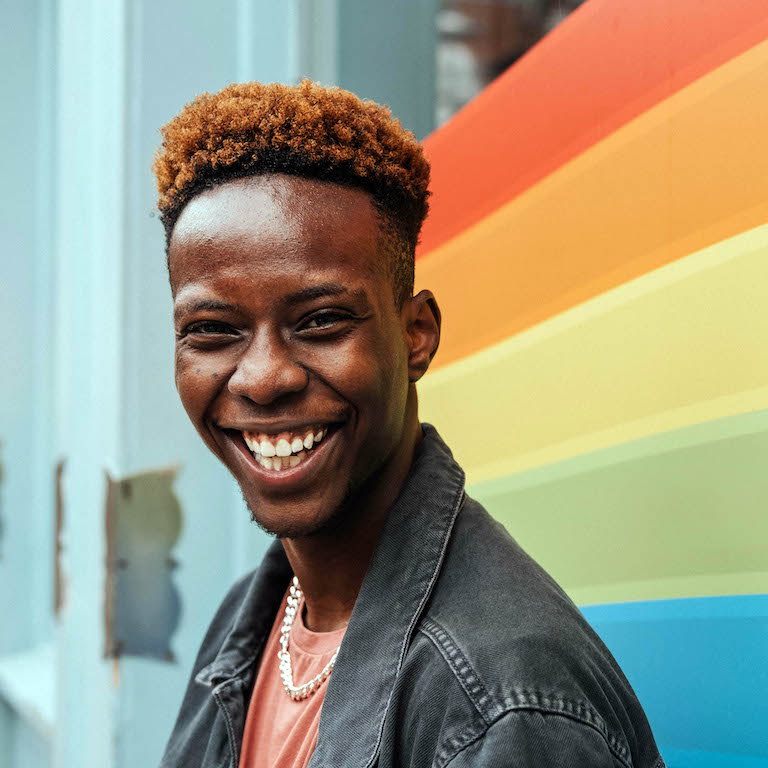
\includegraphics[width=2.8cm, height=2.8cm]{fig/teaser/teaser_1_in.jpg} & $\rightarrow$ & 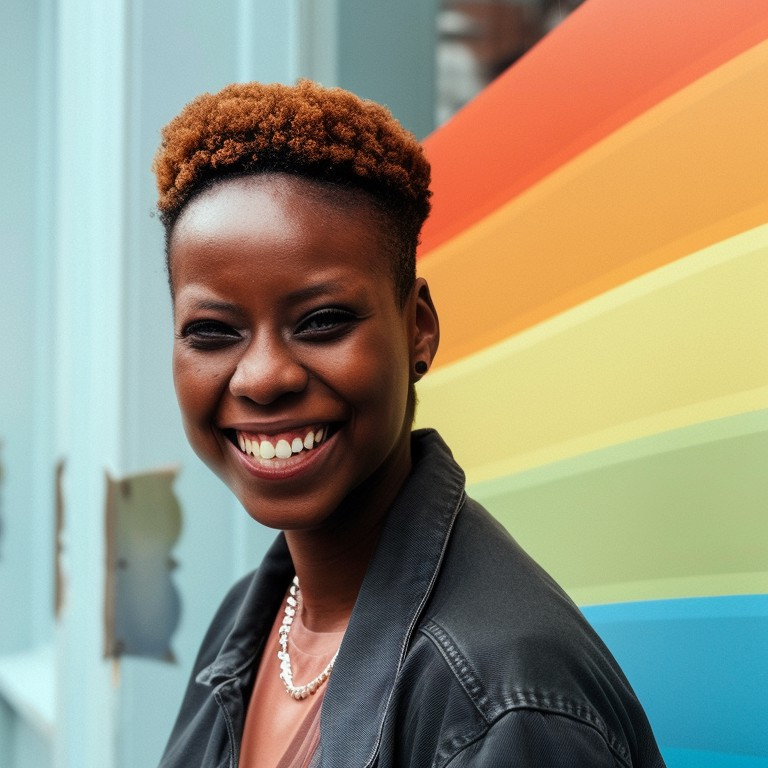
\includegraphics[width=2.8cm, height=2.8cm]{fig/teaser/teaser_1_out} \\
      \multicolumn{3}{c}{``\textit{a \textcolor{BrickRed}{\st{man}} \textcolor{RoyalBlue}{\textbf{woman}} smiling}"} \\
      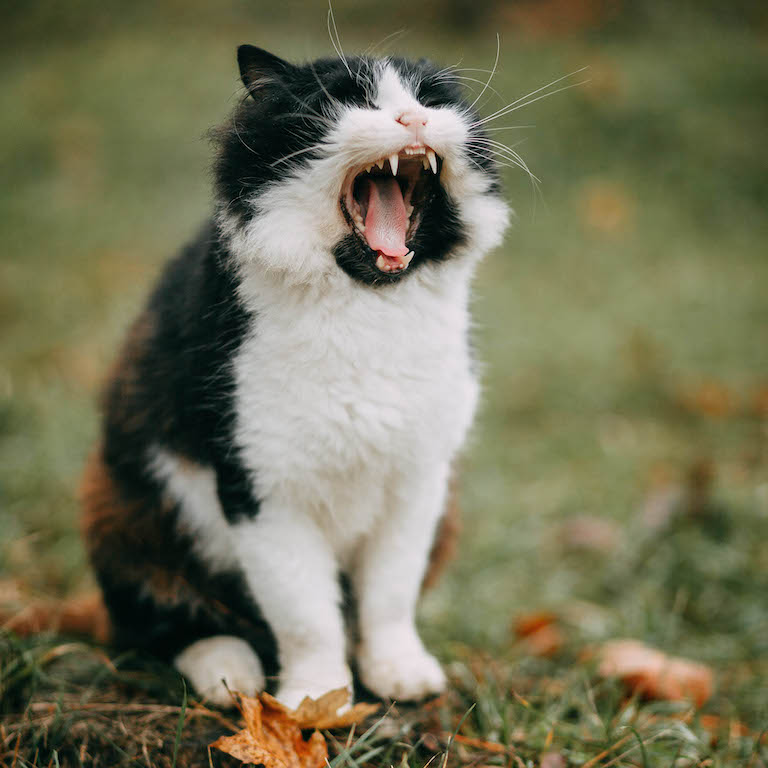
\includegraphics[width=2.8cm, height=2.8cm]{fig/teaser/teaser_2_in.jpg} & $\rightarrow$ & 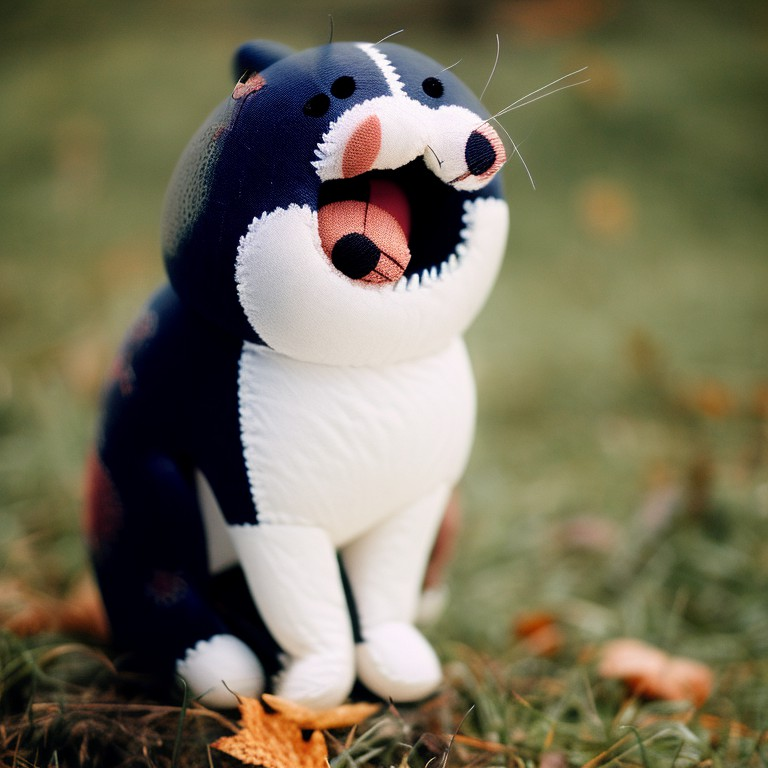
\includegraphics[width=2.8cm, height=2.8cm]{fig/teaser/teaser_2_out} \\
      \multicolumn{3}{c}{``\textit{a \textcolor{RoyalBlue}{\textbf{plush toy}} cat yawning }"} \\
      
    \end{tabular}
    \caption{Prompt-based image editing: the user can add, omit, change, or enhance elements in an image by providing a descriptive prompt of the original image and marking the words that must be removed (in \textcolor{BrickRed}{\textbf{red}}) or added (in \textcolor{RoyalBlue}{\textbf{blue}}).}
    \label{fig:teaser}
  \end{figure}
  

  \begin{figure*}[ht]
    \centering
    % import pdf≤
    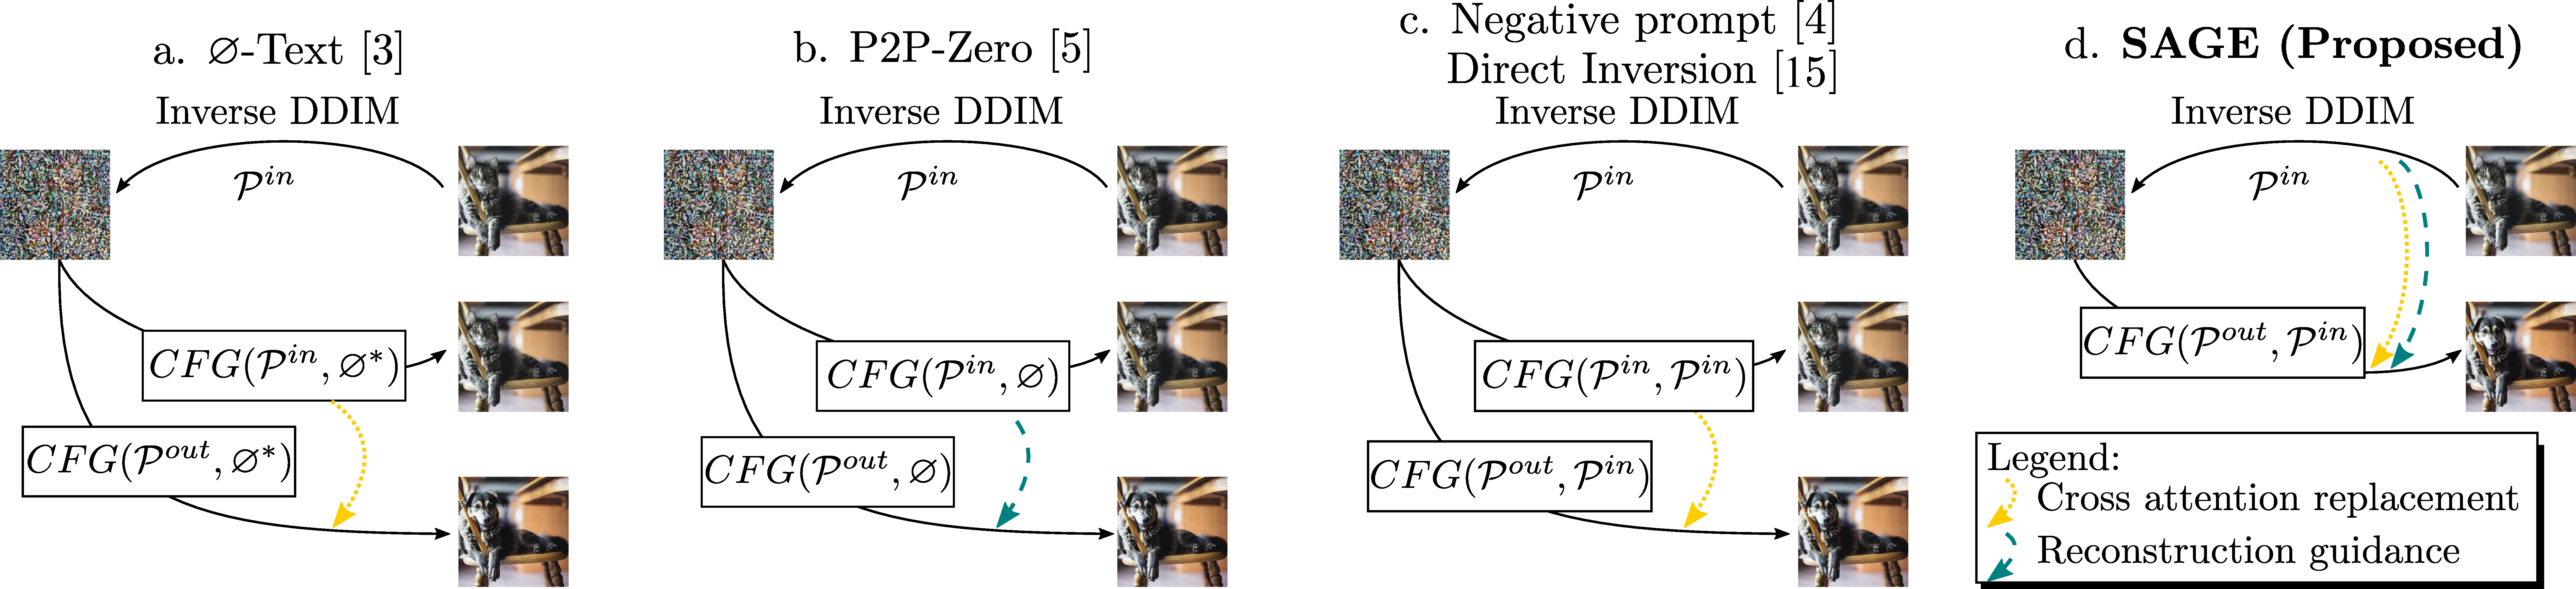
\includegraphics[width=0.9\linewidth]{fig/related.pdf}
    \caption{Comparative Analysis of Diffusion-Based Image Editing Techniques. {\modified{}This review contrasts} existing methodologies, which utilize Classifier-Free Guidance (CFG) \cite{ho2021classifier} with various combinations, including the pretrained null-prompt $\varnothing$, an optimized latent representation $\varnothing^*$, the descriptive prompt of the input image $\pin$, and the target editing prompt $\pout$. 
    }
      \label{fig:related}
    \end{figure*}
  

To address these challenges, {\modified{}this paper introduces} \method{}  (Self-Attention Guidance for Editing), a novel method that reconciles the requirements for computational efficiency and high-fidelity reconstruction, while affording flexible image editing capabilities. Our approach, akin to existing methodologies~\cite{mokady2023null,miyake2023negative,parmar2023zero}, leverages Denoising Diffusion Implicit Model (DDIM) \cite{song2021ddim} inversion. However, it uniquely exploits the intermediate self-attention and cross-attention maps internally computed by the diffusion model during the inverse DDIM process, enabling faithful reconstruction with minimal computational overhead. During the sampling process from random noise to the output image, {\modified{}our method benefits} from a synergistic application of Classifier-Free Guidance (CFG, see Sec~\ref{sec:self_attention_guidance}) alongside a novel reconstruction guidance mechanism based on self-attention reconstruction. This mechanism operates on the self-attention maps within the diffusion U-Net~\cite{ronneberger2015unet}, facilitating a fine trade-off between editing and preservation of the original image details.

In summary, our contribution is threefold:


\begin{itemize}
    \item {\modified{}Introduction of} a novel editing framework utilizing a pre-trained diffusion model that leverages intermediate noise vectors from the inverse DDIM process. This enables the reconstruction to be steered toward the input image, while allowing modifications aligned with textual prompts.
    \item {\modified{}Proposal of} a reconstruction guidance loss term that operates in the self-attention layers of the diffusion network. This term ensures high-fidelity reconstruction in regions unaffected by the editing process without adding major computational overhead.
    \item {\modified{}Experimental validation benchmarks our approach} against recent methods in the field. \method{} outperforms other methods not only in quantitative and qualitative evaluations but also in a comprehensive user study, where it was preferred in over 60\% of cases. Additionally, it ranked first in seven out of 10 quantitative assessments, securing second and third places in the remaining ones.
\end{itemize}




\section{Related Works}
\label{sec:related}

With the impressive advancements in text-to-image diffusion models~\cite{rombach2022latent}, there has been a growing interest in exploring image editing using pre-trained diffusion models. These studies have introduced several editing tasks where the user can guide the generated image through various inputs. For instance, SDEdit~\cite{meng2022sdedit} allows users to apply brush strokes to areas they wish to edit. The model then injects random noise into these targeted areas and uses the diffusion process for denoising. To create new images from examples, techniques like Textual Inversion~\cite{gal2023textual} and Dream-Booth~\cite{ruiz2023dreambooth} employ gradient-descent-based optimization to learn personalized concepts. Text-based editing, in particular, has garnered considerable interest due to its intuitive and user-friendly interaction style. In this domain, DiffusionCLIP~\cite{kim2022diffusionclip} uses DDIM inversion~\cite{song2021ddim} to reverse the diffusion process and applies fine-tuning. This approach guides the generation with a CLIP-based loss to align the generated image more closely with the intended edit.
Another method, as demonstrated in ControlNet~\cite{zhang2023adding}, involves conditioning the generation process on the edges or pose information extracted from the input image. This technique aims to generate an image that retains the original spatial structure yet {\modified{}is styled} according to the given prompt.

  \begin{figure*}[ht]
    \centering
    % import pdf
    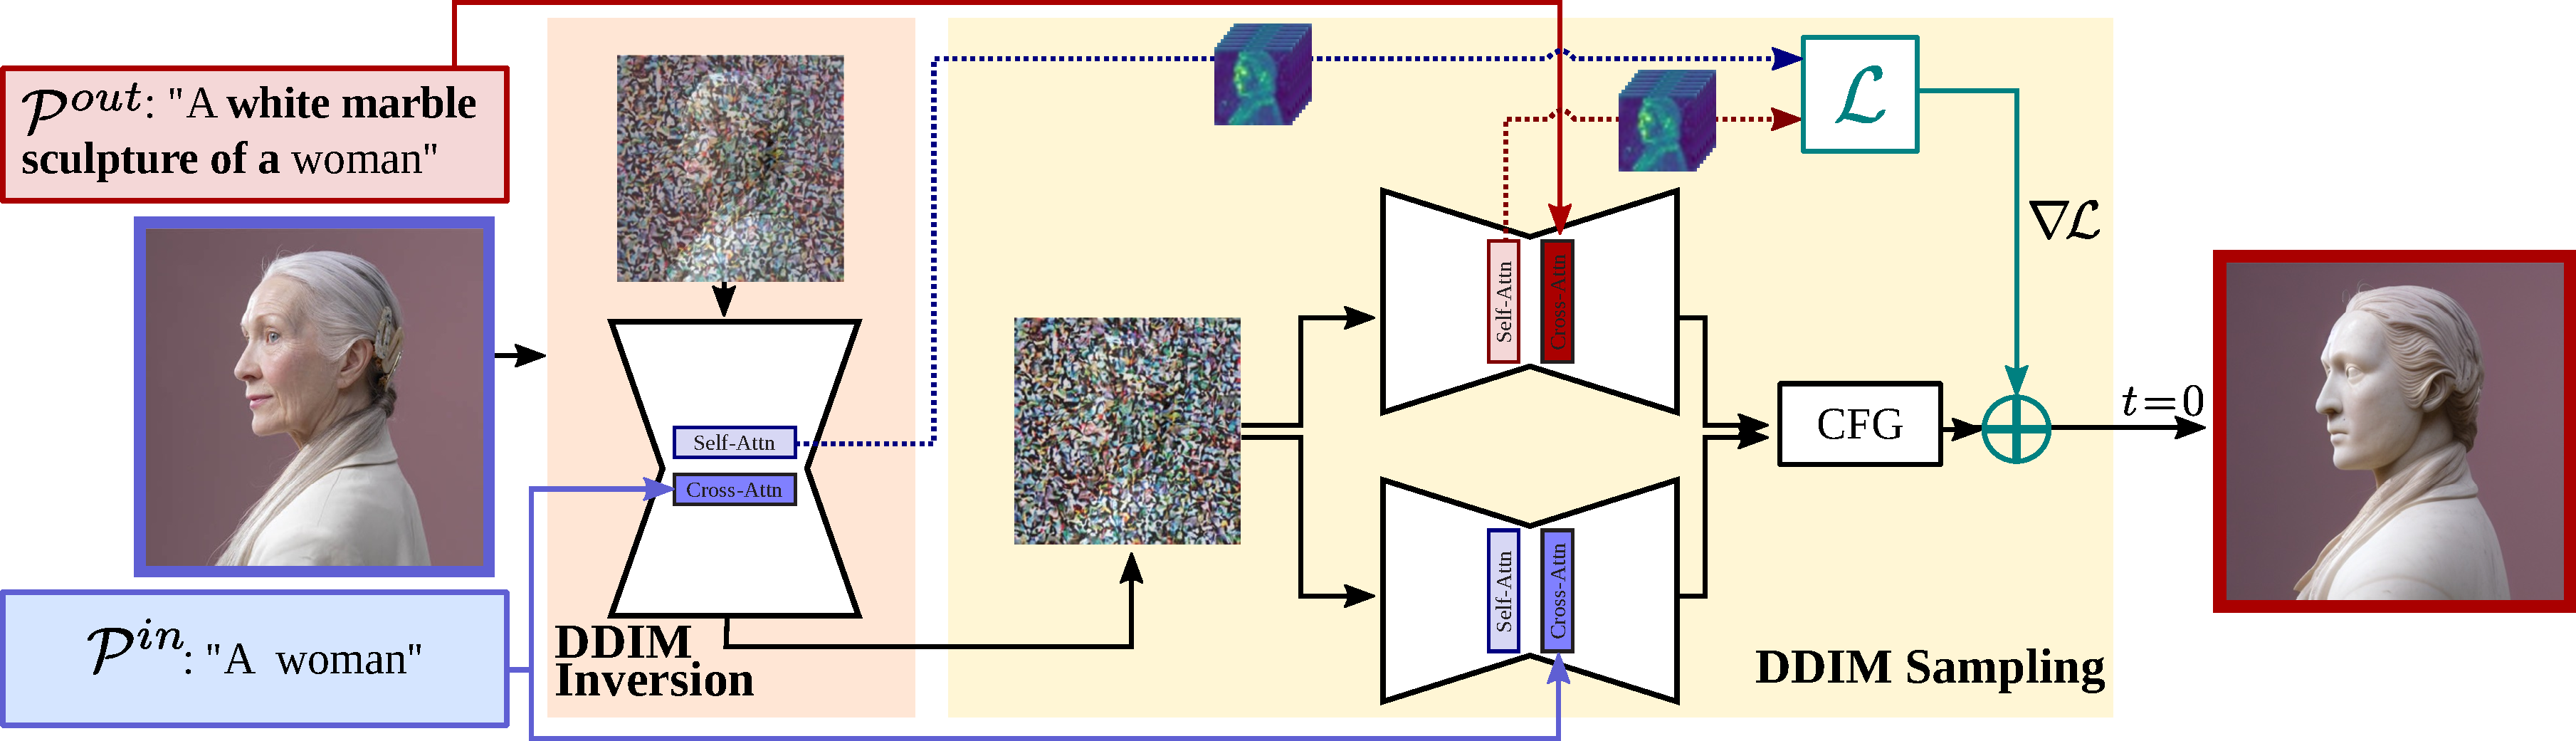
\includegraphics[width=0.85\linewidth]{fig/pipeline.pdf}
      
    \caption{
      Pipeline of \method{}: The process begins with DDIM inversion applied to the input image using its corresponding prompt, $\pin$. This inversion yields the estimated noise $\vz_T$, which serves as the initial condition for the DDIM sampling process responsible for generating the edited image. The U-Net processes both the editing prompt $\pout$ and the initial prompt $\pin$ separately, implementing classifier-free guidance. To enhance reconstruction and mitigate inaccuracies introduced by DDIM inversion, a guidance term is computed. This term is derived by comparing the self-attention maps from the DDIM inversion with those estimated by the U-Net when conditioned on the initial prompt $\pin$, ensuring closer alignment and improved fidelity in the final output.
    }
      \label{fig:method_diag}
\end{figure*}
    
{\modified{}This work focuses} on the prompt-based editing task as formulated in \cite{mokady2023null}. In this task (see Fig.~\ref{fig:teaser}) a user provides an image along with a textual prompt  $\pin$, which describes the input image. The user can then instruct the model to add, remove, change, or enhance elements in the image by providing a target prompt $\pout$ corresponding to the desired image (also called positive prompt). This problem formulation has inspired several subsequent studies~\cite{mokady2023null,parmar2023zero,tumanyan2023plug,ju2023direct}.
{\modified{}A high-level comparison is presented}  in Fig.~\ref{fig:related}, where all methods use CFG for conditioned generation and employ a mechanism to reverse the diffusion process, enabling the reconstruction of the input image from Gaussian noise. These approaches vary in their inversion mechanisms and CFG prompting strategies.

In the \nulltextlong{} (\nulltext) (see Fig.~\ref{fig:related}a), Mokady \etal{} \cite{mokady2023null} optimize the null prompt embedding fed to the diffusion model for input reconstruction, with editing facilitated via a cross-attention mechanism \cite{hertz2023prompt}. In \ptopzerolong{} \cite{parmar2023zero} (Fig.~\ref{fig:related}b), the computationally intensive inversion process is bypassed by introducing a guidance term at each diffusion step, steering the model toward accurate reconstruction. Conversely, \negativelong{} (\negative) \cite{miyake2023negative} (Fig.~\ref{fig:related}c) replaces the conventional CFG's null prompt with a negative prompt, with editing achieved through cross-attention manipulation \cite{hertz2023prompt, mokady2023null}. In \directinversionlong{} (\directinversion) \cite{ju2023direct} (Fig.~\ref{fig:related}c), the authors propose a direct inversion method that corrects the reconstruction process and introduces an edit benchmark. 
More recently, EDICT \cite{wallace2023edict} and BDIA \cite{zhang2024exact} have advanced exact diffusion inversion methods using coupled transformations and bidirectional integration approximation, respectively.


\section{Method}
\label{sec:method}

{\modified{}This work addresses} the prompt-based image editing task as introduced in \cite{hertz2023prompt,mokady2023null} (see Fig.~\ref{fig:teaser}): the user provides an input image $\vi$ alongside a textual prompt $\pin$ that describes the input image. The user also provides a target prompt $\pout$ which describes the image to obtain after editing.
To address this task, {\modified{}this paper introduces} \method, a method based on Self-Attention Guidance for image Editing whose main pipeline is depicted in Fig.~\ref{fig:method_diag}. 
{\modified{}The proposed approach} (Fig.~\ref{fig:related}d) diverges from the compared methods in two main aspects: (i) {\modified{}it achieves} effective editing without the explicit reconstruction of the input image; other works that do not enforce reconstruction usually achieve good editing performance, but the original image content is poorly preserved \cite{tumanyan2023plug} or {\modified{}requires} additional clues for reasonable structure conservation \cite{xu2023inversion}. (ii) {\modified{}it leverages} intermediate self-attention latent maps computed during the inverse DDIM process to guide the generation, this semantically rich and stable latent space (unlike noisy and arbitrary VAE latent space) enables editing while preserving the content in regions unaffected by the edit. This results in a simpler, more powerful, and computationally efficient method.


{\modified{}The proposed method assumes} a pre-trained text-to-image diffusion model~\cite{ho2020ddpm,saharia2022imagen}. In particular, {\modified{}it employs} a latent diffusion model which operates in the latent space of a pre-trained autoencoder~\cite{rombach2022latent}.
Diffusion models are generative models that employ a neural network as a noise predictor, $\varepsilon_\theta^t(\vz_t,\mathcal{P})$, tasked with the restoration of gradually noised data points at various time steps denoted by ${t \in[0,T]}$. Here, $\vz_t$ represents the noise-altered version of the initial sample $\vz_0$, expressed as $\vz_t = \sqrt{\alpha_t} \vz_0 + \sqrt{1-\alpha_t} \varepsilon$, where $\varepsilon$ is the added Gaussian noise. The noise level is controlled by the variable $\alpha_t$, which ranges from nearly 1, indicating no noise, to almost 0, denoting complete Gaussian noise, as time progresses from $1$ to $T$. Additionally, $\mathcal{P}$ is an optional conditioning variable which, in {\modified{}this} case, takes the form of a textual prompt.  The network $\varepsilon_\theta^t(\vz_t,\mathcal{P})$ is implemented with a U-Net equipped with both self-attention and cross-attention layers~\cite{vaswani2017attention} which process the conditioning information.


{\modified{}Following} previous works~\cite{preechakul2021diffusion, mokady2023null, miyake2023negative}, {\modified{}this paper adopts a widely used} variant of diffusion models known as DDIM that enables faster sampling \cite{song2021ddim}.

  
{\modified{}A pre-trained encoder} $Enc(\cdot)$ {\modified{}projects} the input image $\vi$ into the latent space, $\zddim_0=Enc(\vi)$, and apply deterministic DDIM inversion \cite{song2021ddim} to reverse the diffusion process. Given the input prompt $\pin$,  DDIM inversion gives {\modified{}a reversed} sequence of noisy latent variables $\zddim_{t}$, where $t$ increases from $0$ to $T$
 
\begin{align}
        \label{eq:ddim_inversion}
        \zddim_{t+1}=&\frac{\sqrt{{\alpha}_{t+1}}}{\sqrt{{\alpha}_{t}}} (\zddim_{t}-\sqrt{1-{\alpha}_{t}}\varepsilon_{\theta}^{t}(\zddim_{t},\mathcal{P}))\notag\\
        &+\sqrt{1-{\alpha}_{t+1}}\varepsilon_{\theta}^{t}(\zddim_{t},\pin)
      \end{align}


      \begin{figure}[h]
  \centering

   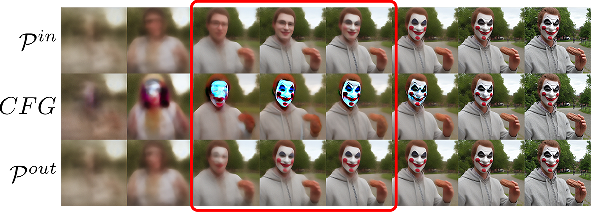
\includegraphics[width=0.8\linewidth]{fig/CFG.pdf}

   \caption{
      Positive and Negative prompt $\hat \vz_0$ estimation across timesteps. We visualize the estimated $\hat \vz_0$ for positive $\pout$, negative prompt $\pin$, and CFG  (both $\pout$ and $\pin$) during DDIM sampling with CFG.
   }
   \label{fig:posneg_direction}
\end{figure}

\subsection{Self-Attention Guidance}
\label{sec:self_attention_guidance}

{\modified{}This paper proposes} two complementary guidance mechanisms to simultaneously achieve effective editing—altering the image to match the target prompt $\pout$—and faithful reconstruction—preserving key regions of the input image.

For editing, {\modified{}a variant of classifier-free guidance (CFG) is adopted} \cite{miyake2023negative}

\begin{align}
  \label{eq:cfg}
    \begin{split}
      \tilde{\varepsilon}_{\theta}^{t}(\vz_{t},&\pin,\pout)= \varepsilon_{\theta}^{t}(\vz_{t},\pin)\\
      &+ w \cdot \left( \varepsilon_{\theta}^{t}(\vz_{t},\pout) - \varepsilon_{\theta}^{t}(\vz_{t},\pin) \right) 
    \end{split}
\end{align}
with $w>0$ modulating the balance between the two objectives. As illustrated in Fig.~\ref{fig:posneg_direction}, early in the diffusion process, the noise estimates for $\pin$ and $\pout$ both steer $\hat{\vz}_t$ toward the original image; then diverge: $\varepsilon_{\theta}^{t}(\vz_{t},\pin)$ favors reconstruction while $\varepsilon_{\theta}^{t}(\vz_{t},\pout)$ drives the editing transformation. 
As $t$ approaches 1, these estimates converge, resulting in a final image that balances input fidelity with the desired prompt edits.
In practice, an excessively low $w$ results in over-reconstruction, whereas a very high $w$ may neglect crucial details of the input image.

To promote reconstruction without resorting to explicit optimization or direct latent-space comparisons (which can cause diffusion instability), {\modified{}the proposed method leverages} the self-attention maps within the U-Net architecture. Unlike cross-attention—which only associates textual tokens with specific image regions \cite{hertz2023prompt,han2023proximal}—self-attention encodes global interactions among all image tokens, capturing richer spatial relationships that are essential for preserving image details not explicitly mentioned in the prompt. Concretely, during DDIM inversion, {\modified{}self-attention maps} $S_{i,t}^{in}$ {\modified{}are recorded} for each transformer block, and during synthesis, {\modified{}corresponding maps} $S_{i,t}^{out}$ {\modified{}are collected} from $\varepsilon_{\theta}^{t}(\vz_{t},\pout)$. {\modified{}Reconstruction is then enforced} by minimizing the loss
\begin{equation}
    \label{eq:self_attention_guidance}
    \mathcal{L}^\text{self}_t =  \sum^N_i \|S_{t,i}^{in} - S_{t,i}^{out}\|_1.
\end{equation}
This loss gradient, scaled by a factor $\lambda$, is incorporated into the noise update
\begin{equation}
    \hat{\vz}_{t-1} = \vz_{t-1} - \lambda \nabla_{\vz_t}\mathcal{L}^\text{self}_t.
\end{equation}
Following \cite{couairon2023monotonical}, {\modified{}factor} $\lambda$ progressively decreases with $t$, so that early diffusion steps emphasize the editing transformation while later steps focus on denoising and fine reconstruction.

In contrast to existing methods that require explicit reconstruction optimization \cite{mokady2023null,miyake2023negative} or depend solely on cross-attention for guidance, {\modified{}the presented approach integrates} self-attention guidance to capture all necessary information from the DDIM inversion. This strategy not only stabilizes the reverse diffusion process but also achieves a more robust and balanced trade-off between editing and reconstruction, thereby differentiating {\modified{}this contribution} from prior work.

% \setlength{\tabcolsep}{1pt}
\begin{figure}[h]
    \small
    \centering
    \begin{tabular}{ccc}
      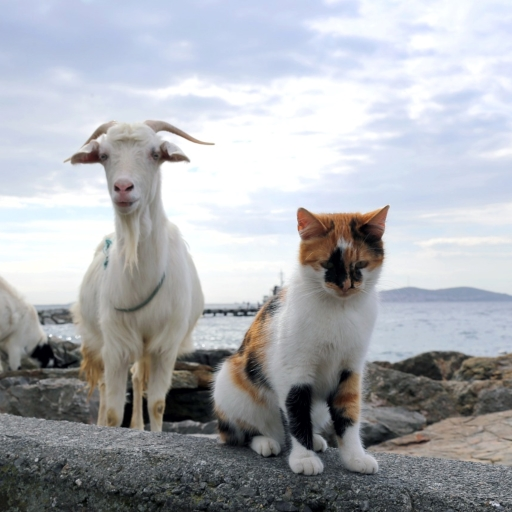
\includegraphics[width=1.8cm, height=1.8cm]{fig/cross_map_images/cross_image} & 
\includegraphics[width=1.8cm, height=1.8cm]{fig/cross_map_images/cat_map} & 
\includegraphics[width=1.8cm, height=1.8cm]{fig/cross_map_images/goat_map} \\
      Input & \textit{``cat"} & \textit{``goat"} \\
    %   \multicolumn{3}{c}{``\textit{a \textcolor{BrickRed}{\st{man}} \textcolor{RoyalBlue}{\textbf{woman}} smiling}"} \\
    %   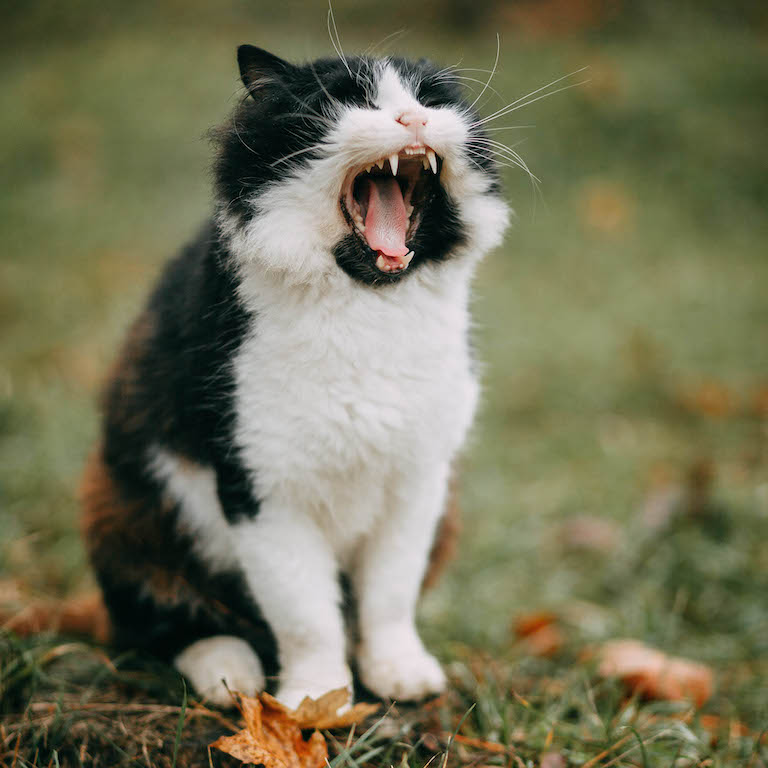
\includegraphics[width=2.2cm, height=2.2cm]{fig/teaser/teaser_2_in.jpg} & $\rightarrow$ & 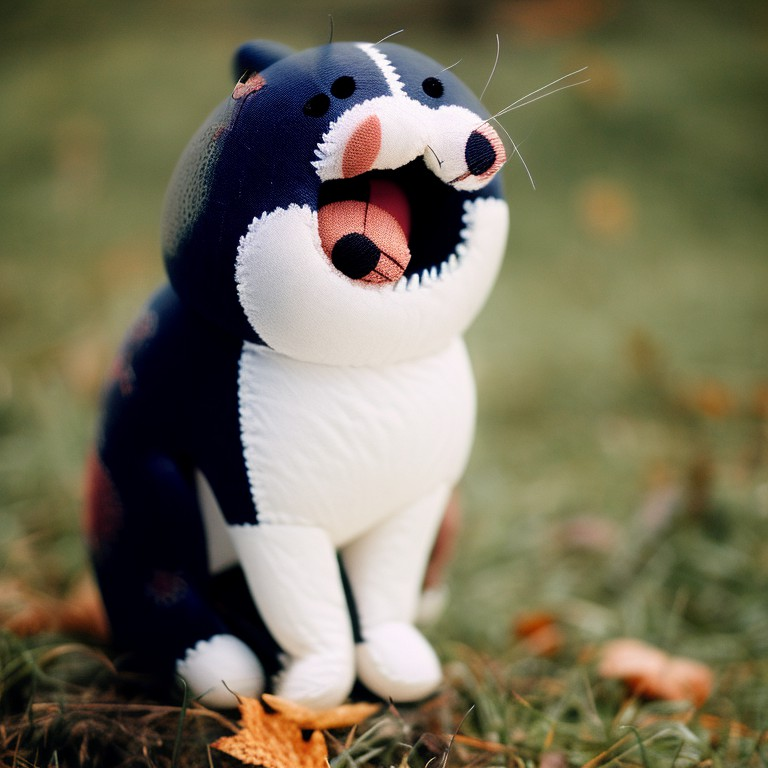
\includegraphics[width=2.2cm, height=2.2cm]{fig/teaser/teaser_2_out} \\
    %   \multicolumn{3}{c}{``\textit{a \textcolor{RoyalBlue}{\textbf{plush toy}} cat yawning }"} \\
      
    \end{tabular}
    \caption{Averaged $16 \times 16$ cross-attention maps corresponding to ``\textit{cat}" and ``\textit{goat}" for the input ``\textit{A cat and a goat}."}
    \label{fig:crossatt_map}
  \end{figure}

%   \begin{figure}
%     \includegraphics[width=0.99\linewidth]{fig/03_bird_and_bear.pdf}
%     \caption{Averaged cross-attention maps for the sentence "a furry bear watching a bird". The cross-attention maps corresponding to \textit{bird} and \textit{bear} are also shown across different timesteps. Figure taken from \cite{hertz2023prompt}. \guille{This is 100\% stolen from prompt-to-prompt but I believe it's really important for understanding what cross-attention maps are and what do they encode. How critital is that we make our own?}}
%     \label{fig:crossattn_viz}
%   \end{figure}
  


\subsection{Cross-Attention Manipulation}
\label{sec:cross_attention_manipulation}
Following \cite{hertz2023prompt} (see also \cite{mokady2023null,parmar2023zero,han2023proximal,ju2023direct,miyake2023negative}), {\modified{}this method uses} the U-Net’s cross-attention maps—which link latent space coordinates to prompt tokens—to guide the structural editing process. {\modified{}Proposed} adaptations include three mechanisms:


\textbf{Local Blending.} To recover fine details (e.g., colors and textures) that may be lost with self-attention alone, {\modified{}a high-resolution blending mask is derived} from the cross-attention maps. {\modified{}The maps from both the original prompt} $\pin$ and the editing prompt $\pout$ {\modified{}are aggregated} across diffusion steps and U-Net layers, then normalized, thresholded, and upscaled to obtain a binary mask $M$. This mask is used to fuse the edited latent $\vz_{t-1}$ with the original latent $\zddim_{t-1}$

\begin{equation}
    \label{eq:local_blend}
    \hat{\vz}_{t-1} = M \odot \vz_{t-1} + (1-M) \odot \zddim_{t-1}.
\end{equation}
This approach enhances detail preservation and improves computational efficiency by leveraging a single CFG estimation.

\textbf{Cross-Attention Replacement.} When $\pout$ involves a word swap in $\pin$, {\modified{}the shape of the modified object is preserved} by replacing the cross-attention maps for the altered token. Specifically, for token $k$, {\modified{}the method substitutes} $C_{t,i}^{out}[k]$ with $C_{t,i}^{in}[k]$ during the early diffusion stages (roughly the first 20\%), balancing shape retention with overall image quality.

\textbf{Cross-Attention Reweighting.} Finally, users can adjust the influence of specific words by reweighting the corresponding cross-attention maps $C_{t,i}^{out}[k]$, offering fine-grained control over the editing outcome.

These mechanisms, derived with minor adaptations from \cite{hertz2023prompt}, complement {\modified{}the presented framework} by refining structural guidance and detail preservation during image synthesis.

\section{Experiments}
\label{sec:experiments}
Every \method{} experiment was run on a single NVIDIA A100-40GB of a DGX A100 server. All code for generation, experimentation, evaluation, and ablation studies {\modified{}is} available at \codeurl.
The images for remaining methods used in the quantitative comparison (Sec~\ref{sec:expsota}) and user study (Sec~\ref{sec:userstudy}) are taken from the PieBench experimentation files \cite{ju2023direct}. The images for the qualitative comparison (Fig.~\ref{fig:method_comparison} and Sec~\ref{sec:expsota}) corresponding to \nulltext{}, \negative{}, and \negprox{} are taken from \cite{han2023proximal}; the rest were generated with the source code of \cite{ju2023direct}, modifying hyperparameters until the best result was achieved.

As discussed in \cite{mokady2023null,han2023proximal}, all compared methods and diffusion models in general \cite{ho2021classifier} are sensitive to hyperparameters, including {\modified{}\method{}}. Nevertheless, for fairness of comparison, all \method{} results in Tables \ref{tab:ablation_piebench}, \ref{tab:comparison_piebench}, and \ref{tab:user_study} are obtained with the same hyperparameters: 50 DDIM steps, CFG scale of 7.5, local blend in the first 40 steps, cross-attention replacement in the first 5 steps, a 200 self-attention guidance scale, and 2.0 cross-attention reweighting, similar to \directinversion{} \cite{ju2023direct} configuration.


Every method uses $512 \times 512$ images and Stable Diffusion 1.4 as base diffusion model except \pnplong{}, {\modified{}which} uses 1.5. The images in Fig.~\ref{fig:teaser} are $768 \times 768$ images generated using Stable Diffusion 2.1 as the backbone of \method{}.

  
 \setlength{\tabcolsep}{1pt}

  \begin{figure*}[h]
    \footnotesize
    \small
    \centering
    \begin{tabular}{ccccccc}
      \hline

      \multirow{2}{*}{Input} &  (i) & (ii) & (iii) & (iv) & (v) & (vi) \\
      &  CA guidance &  $\vz_t$  guidance & SA replace.&  SA guidance &   (iv)+CA replace. &  (v) + LB \\
      \hline
      \multicolumn{7}{c}{``\textit{a girl with blonde hair \textcolor{RoyalBlue}{\textbf{and a fluffy rainbow hat}} smiling}"} \\
      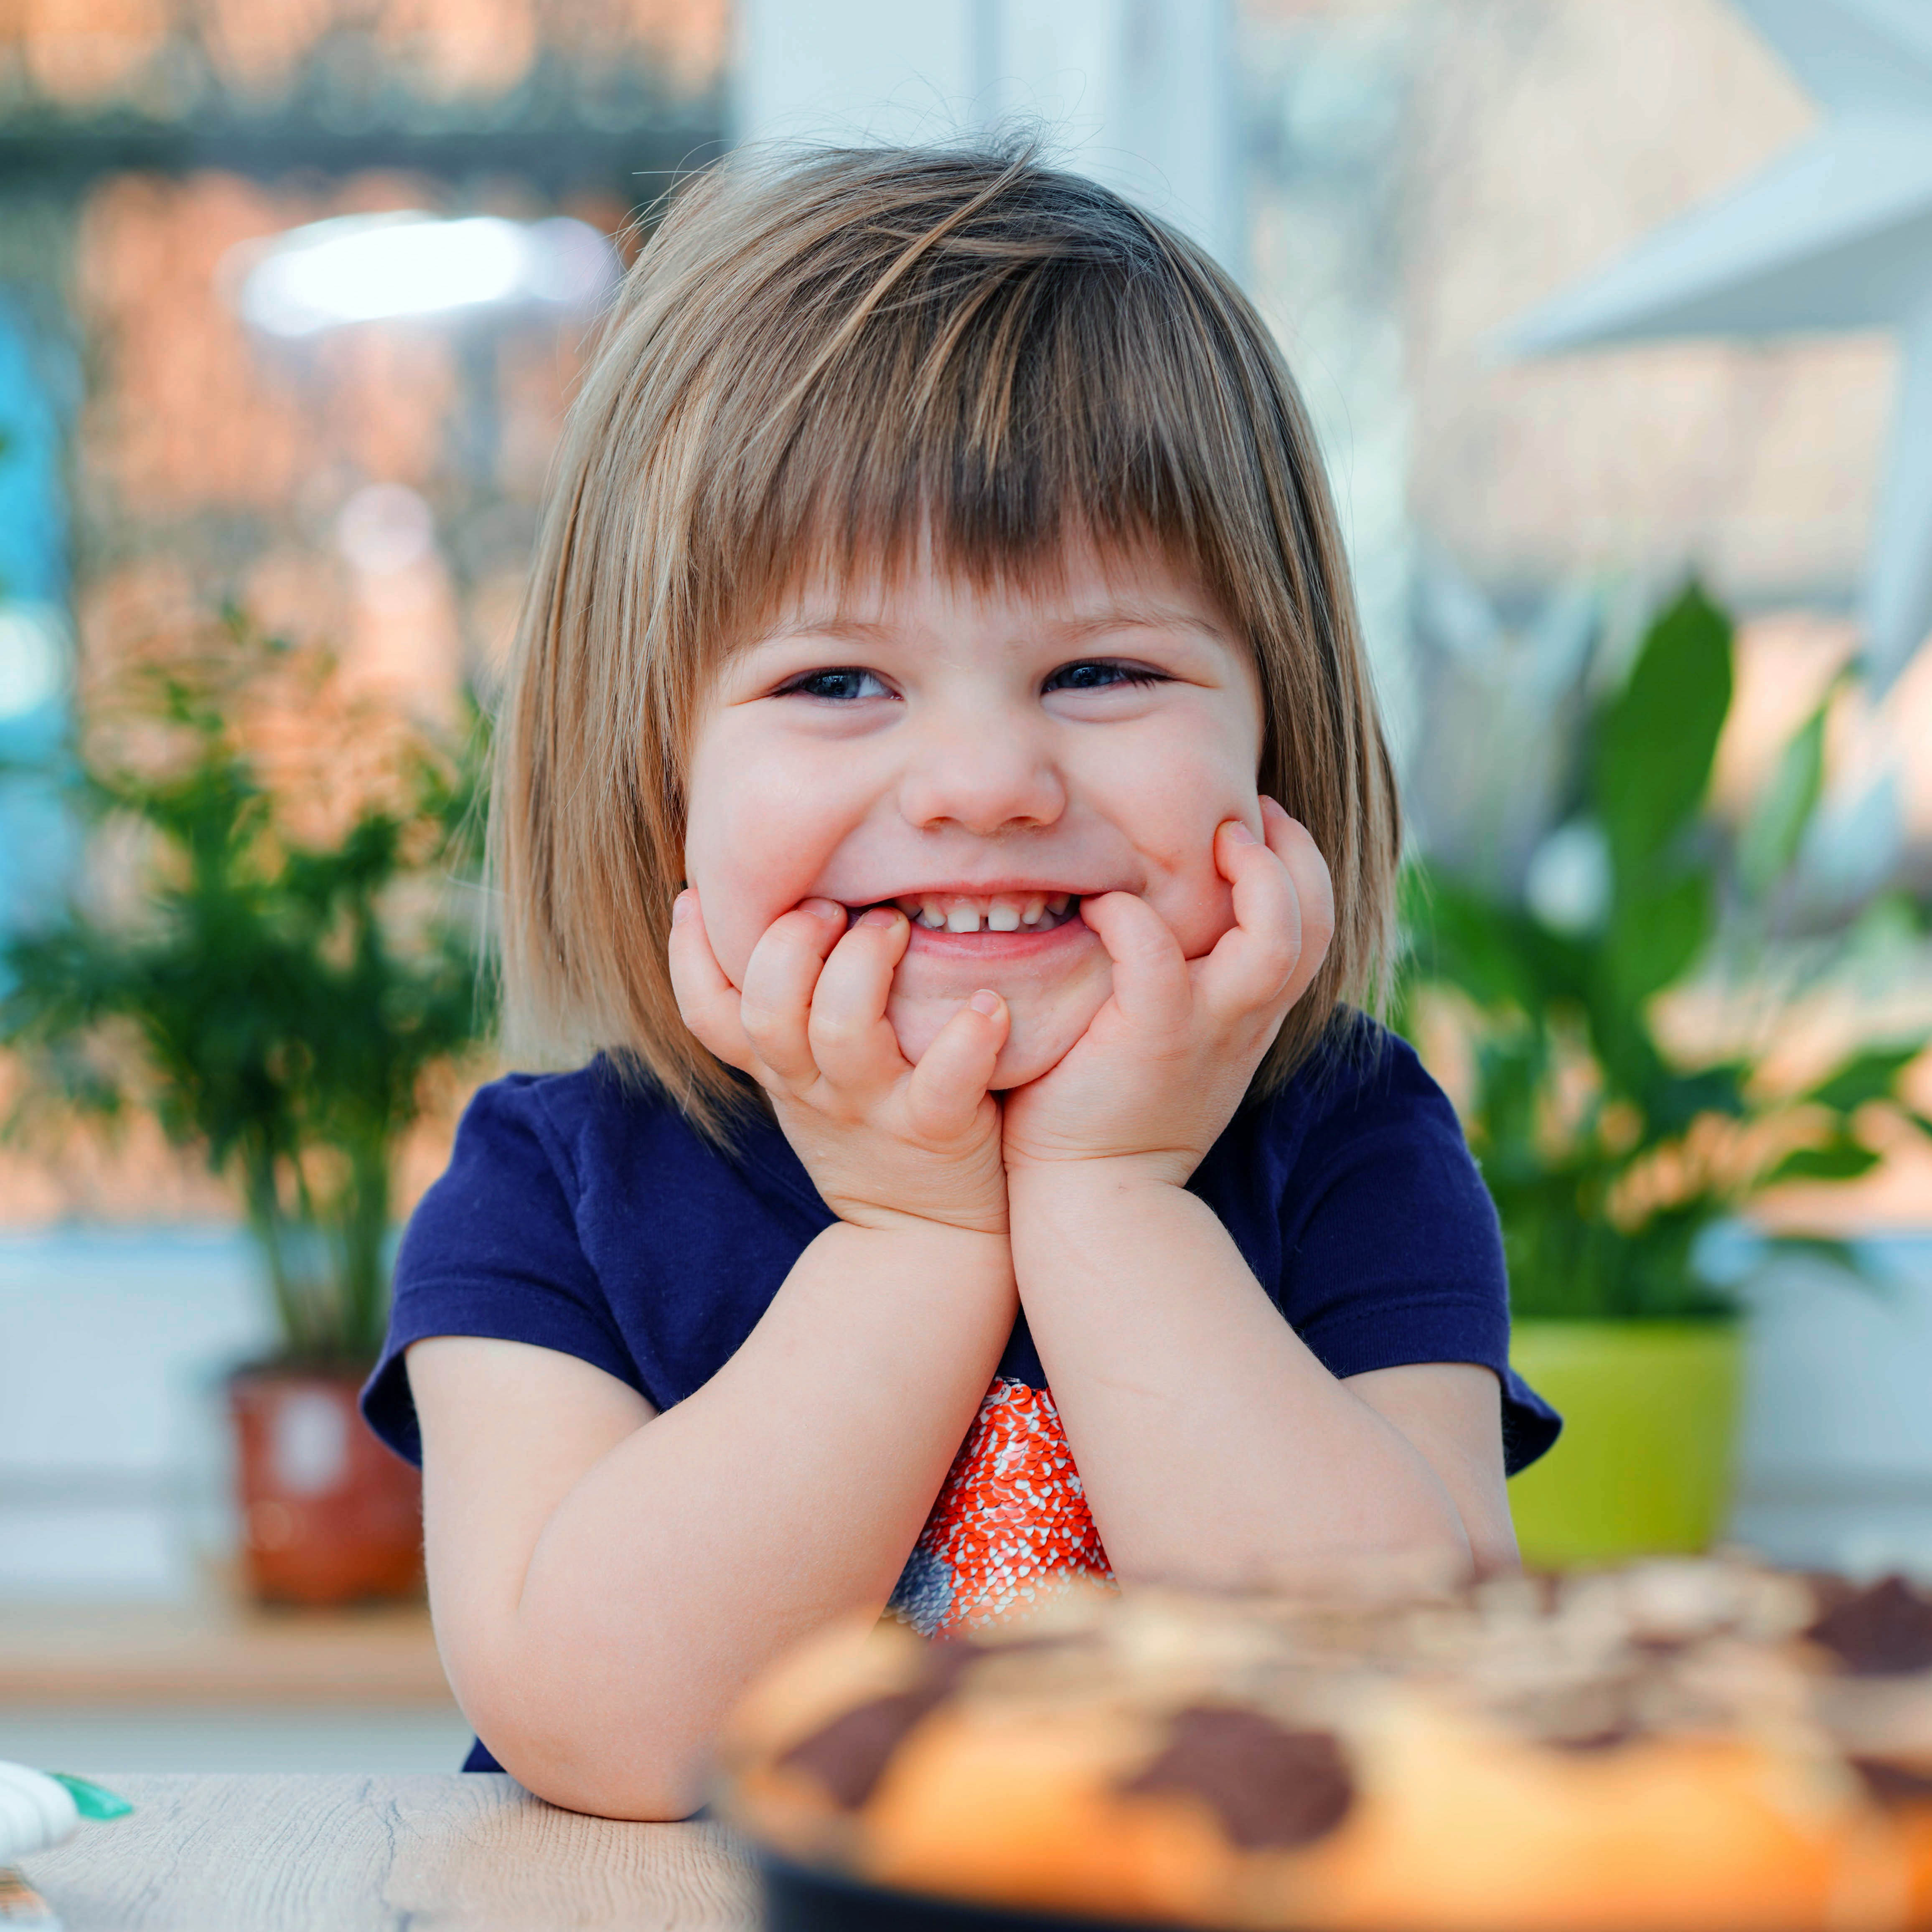
\includegraphics[width=2.1cm, height=2.1cm]{fig/ablation/1_ablation_input} & 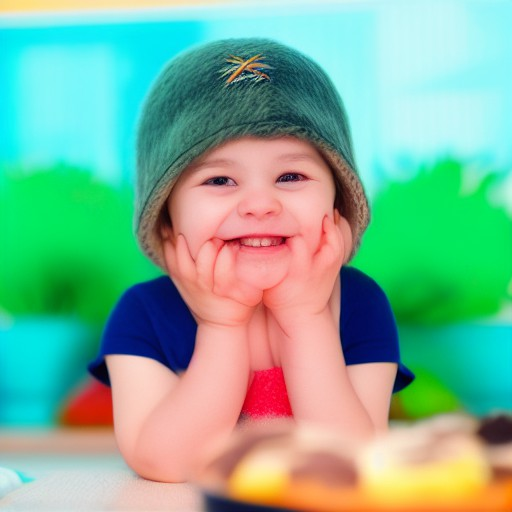
\includegraphics[width=2.1cm, height=2.1cm]{fig/ablation/1_ablation_2} &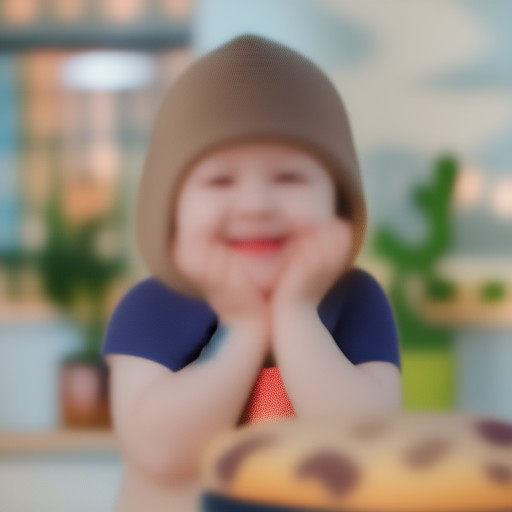
\includegraphics[width=2.1cm, height=2.1cm]{fig/ablation/1_ablation_3} &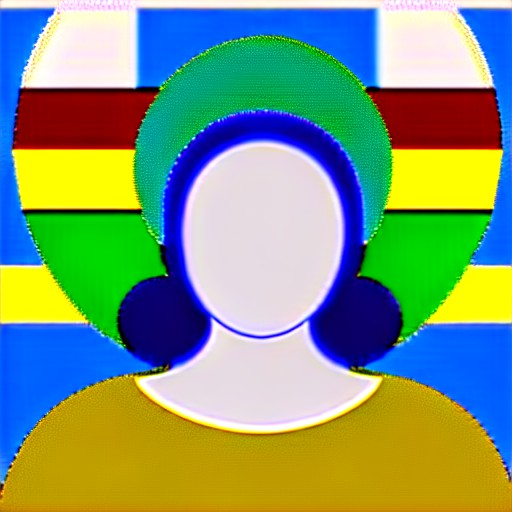
\includegraphics[width=2.1cm, height=2.1cm]{fig/ablation/1_ablation_4_cfg75} &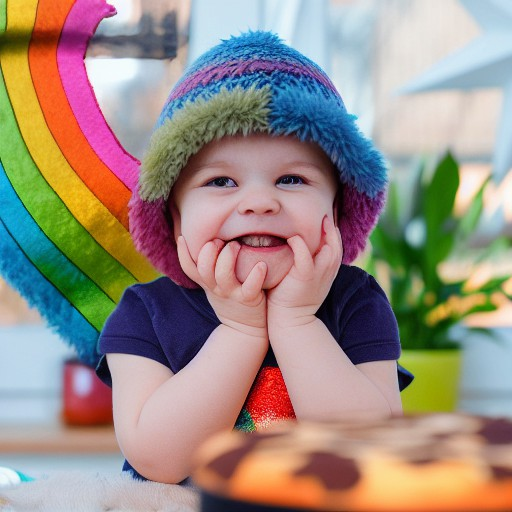
\includegraphics[width=2.1cm, height=2.1cm]{fig/ablation/1_ablation_1} &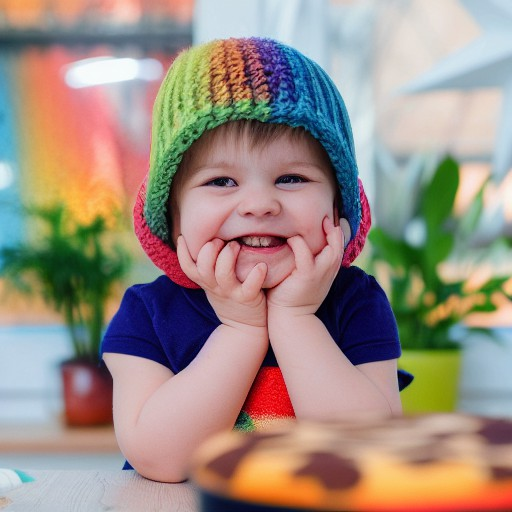
\includegraphics[width=2.1cm, height=2.1cm]{fig/ablation/1_ablation_5} &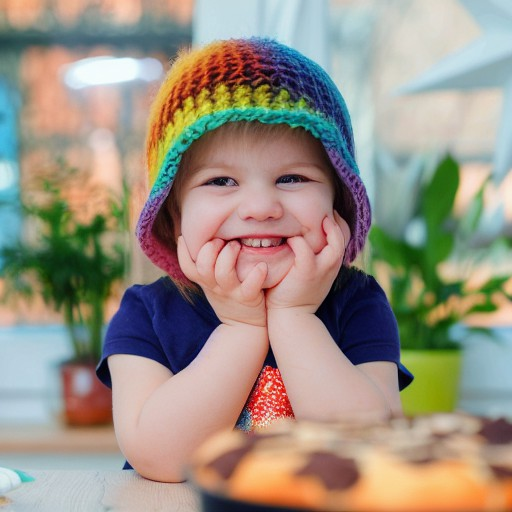
\includegraphics[width=2.1cm, height=2.1cm]{fig/ablation/1_ablation_6} \\
      \multicolumn{7}{c}{``\textit{a baby with a stuffed \textcolor{BrickRed}{\st{monkey}} \textcolor{RoyalBlue}{\textbf{zebra}} in a car}"} \\
      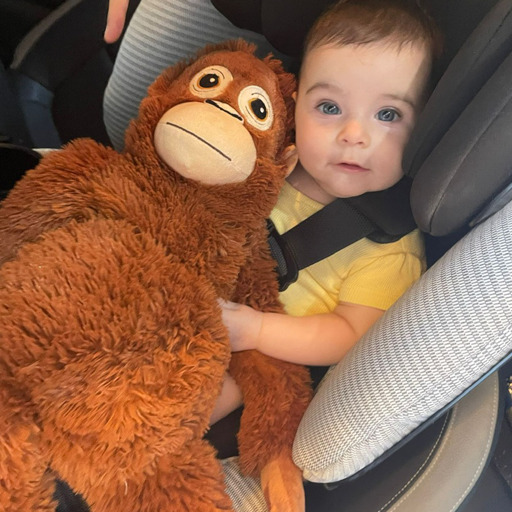
\includegraphics[width=2.1cm, height=2.1cm]{fig/ablation/0_ablation_input} & 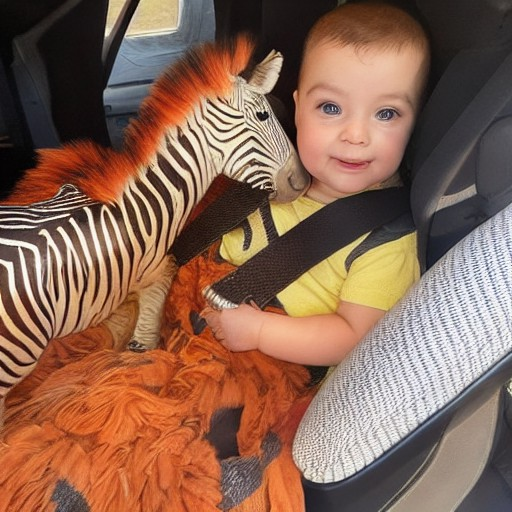
\includegraphics[width=2.1cm, height=2.1cm]{fig/ablation/0_ablation_2} &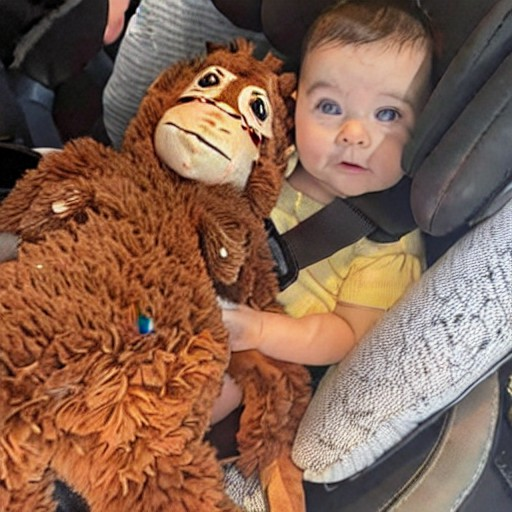
\includegraphics[width=2.1cm, height=2.1cm]{fig/ablation/0_ablation_3} &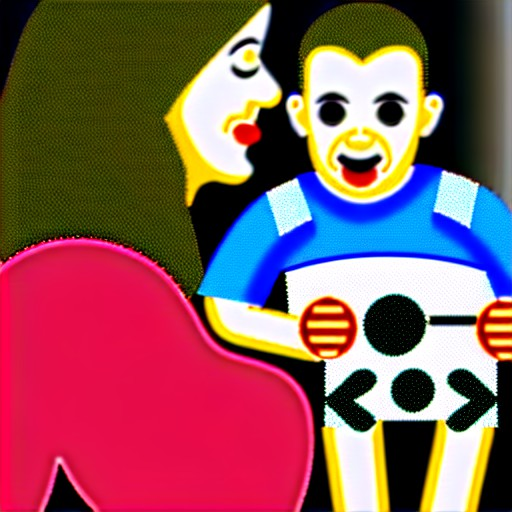
\includegraphics[width=2.1cm, height=2.1cm]{fig/ablation/0_ablation_4}
      &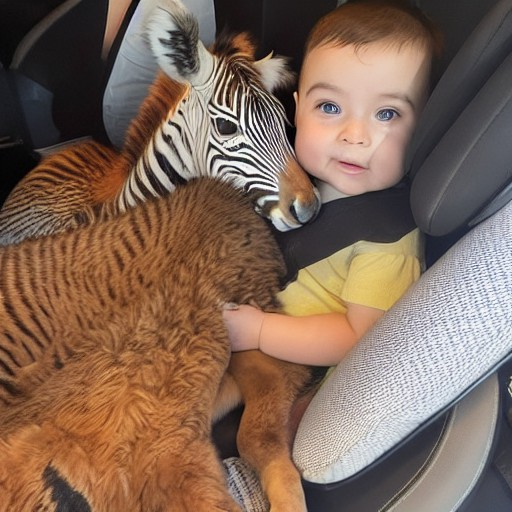
\includegraphics[width=2.1cm, height=2.1cm]{fig/ablation/0_ablation_1} &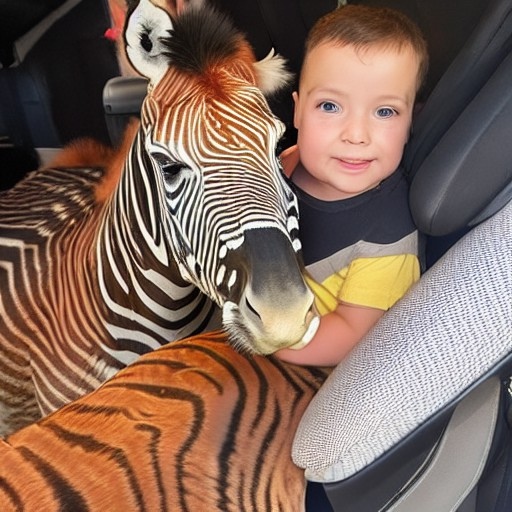
\includegraphics[width=2.1cm, height=2.1cm]{fig/ablation/0_ablation_5} &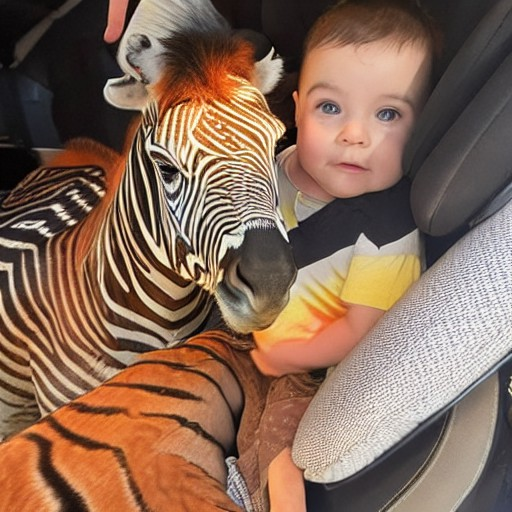
\includegraphics[width=2.1cm, height=2.1cm]{fig/ablation/0_ablation_6} \\
      \hline
      % ... Add more rows as needed
    \end{tabular}
    \caption{{\modified{}Qualitative results of the} ablation study. Each column corresponds to a configuration described in Table \ref{tab:ablation_piebench}.}
    \label{fig:ablationquali}
  \end{figure*}

\subsection{Evaluation}

\paragraph{Data} {\modified{}The analysis is conducted} on PieBench \cite{ju2023direct} and MagicBrush \cite{Zhang2023MagicBrush}. PieBench contains 700 images evenly distributed across natural and artificial scenes in four categories (animal, human, indoor, and outdoor) and 10 editing tasks, including object modification, content changes, and style adjustments. Each image includes source and target prompts, edit subjects, and manually annotated masks for background-preservation evaluation (for applicable tasks).  

MagicBrush, designed for instruction-based image editing, consists of 1053 test images with editing instructions; it also supports prompt-to-prompt editing \cite{hertz2023prompt}. Unlike PieBench, it focuses on small-scale edits in photorealistic images.  

Additionally, {\modified{}high-resolution images from Pexels}\footnote{Images in \url{https://www.pexels.com/} are free for commercial use.} {\modified{}are used} for qualitative evaluation.


\paragraph{Metrics} Following {\modified{}the} PieBench evaluation protocol \cite{ju2023direct}, {\modified{}\method{} is evaluated} using three benchmark categories: \textit{1)} structure distance \cite{tumanyan2022splicing}, \textit{2)} background preservation, and \textit{3)} target-prompt fidelity. Background preservation is measured using LPIPS \cite{zhang2018perceptual} and SSIM \cite{wang2004ssim} on the masked area, while prompt fidelity is assessed via CLIP-T Similarity \cite{we2021clipsim} on the entire image and the edited region.  

Similarly, MagicBrush evaluates methods using five metrics: four for input preservation (L1 and L2 distance, CLIP-I similarity \cite{Zhang2023MagicBrush}, and Dino similarity \cite{caron2021emerging}) and one for prompt fidelity (CLIP-T similarity).

\setlength{\tabcolsep}{1pt}
\begin{figure*}[h]
  \centering
    \footnotesize
    \small
    \resizebox{0.85\textwidth}{!}{
    \begin{tabular}{ccccccccc}
      \hline
      Input & \nulltext & NPI & \negprox & PnP & \directinversion & \ptopzero & \method \\
      \hline
      \multicolumn{8}{c}{``\textit{A \textcolor{RoyalBlue}{\textbf{lego}} cat \textcolor{RoyalBlue}{\textbf{toy}} sitting next to a mirror}"} \\
      % \insertimage{cat}{input} & \insertimage{cat}{null} &\insertimage{cat}{neg} &\insertimage{cat}{prox} &  \insertimage{cat}{pnp} & \insertimage{cat}{direct}& \insertimage{cat}{zero} & \fcolorbox{teal}{teal}{\insertimage{cat}{ours_1}}  \\
      \insertimage{cat}{input} & \insertimage{cat}{null} &\insertimage{cat}{neg} &\insertimage{cat}{prox} &  \insertimage{cat}{pnp} & \insertimage{cat}{direct}& \insertimage{cat}{zero} & \insertimage{cat}{ours_1}  \\
      \multicolumn{8}{c}{``\textit{Orange van with \textcolor{BrickRed}{\st{surfboards}} \textcolor{RoyalBlue}{\textbf{flowers}} on top}"} \\
      \insertimage{van}{input} & \insertimage{van}{null} &\insertimage{van}{neg} &\insertimage{van}{prox} & \insertimage{van}{pnp} & \insertimage{van}{direct}& \insertimage{van}{zero}& \insertimage{van}{ours}  \\
      \multicolumn{8}{c}{``\textit{Meat \textcolor{BrickRed}{\st{balls}} \textcolor{RoyalBlue}{\textbf{shushi}} on white plate}"} \\
      \insertimage{meat}{input} & \insertimage{meat}{null} &\insertimage{meat}{neg} &\insertimage{meat}{prox} & \insertimage{meat}{pnp} & \insertimage{meat}{direct}& \insertimage{meat}{zero}& \insertimage{meat}{ours}  \\
      \multicolumn{8}{c}{``\textit{A \textcolor{BrickRed}{\st{woman}} \textcolor{RoyalBlue}{\textbf{storm-trooper}} with blue hair}"} \\
      \insertimage{girl}{input} & \insertimage{girl}{null} &\insertimage{girl}{neg} &\insertimage{girl}{prox} & \insertimage{girl}{pnp} & \insertimage{girl}{direct}& \insertimage{girl}{zero3}& \insertimage{girl}{ours}  \\
      \multicolumn{8}{c}{``\textit{A \textcolor{BrickRed}{\st{cat}} \textcolor{RoyalBlue}{\textbf{dog}} sitting on a wooden chair}"} \\
      \insertimage{cat2}{input} & \insertimage{cat2}{null} &\insertimage{cat2}{neg} &\insertimage{cat2}{prox} & \insertimage{cat2}{pnp} & \insertimage{cat2}{direct}& \insertimage{cat2}{zero}& \insertimage{cat2}{ours}  \\
      \hline
      % ... Add more rows as needed
    \end{tabular}
    }
    \caption{Qualitative comparison with state-of-the-art {\modified{}methods}. {\modified{}Examples are shown for} both word insertion and word swap.}

    \label{fig:method_comparison}
  \end{figure*}
\subsection{Ablation Study}
\label{sec:expablation}




\begin{table}[htbp]
    \centering
    \small
      \renewcommand\arraystretch{0.8}
      \setlength{\tabcolsep}{0.5mm}{
    \resizebox{\linewidth}{!}{
    \begin{tabular}{llcccccc}
     \toprule
          &\multirow{2}{*}{\textbf{Reconstruction}}&\textbf{CA}&\multirow{2}{*}{\textbf{LB}}&\multirow{2}{*}{ \textbf{Struct.}$\downarrow$}      &  \multirow{2}{*}{\textbf{LPIPS} $\downarrow$}     & \multirow{2}{*}{\textbf{CLIP} $\uparrow$} \\ 
 & & \textbf{replace.}&&&&\\
    \midrule
    
    (i)&CA guidance &- & -& 15.7 & 58 & 21.9 \\
    (ii)&$\vz_t$ guidance &-& -& 40.0 & 111.3 & 21.5 \\
    (iii)&SA replace &- & -&178.4 & 376.0 & 18.8 \\
    (iv)& SA guidance& -& -&  15.7 & 42.0 & \textbf{22.0}  \\
    \midrule
    (v)& SA guidance&\checkmark&- & 14.7 & 49.5 & 21.9 \\
    (vi)& SA guidance&\checkmark&\checkmark & \textbf{11.0} & \textbf{39.6} & \textbf{22.0}\\
    \bottomrule
    \end{tabular}}
  
    }
        % \vspace{-0.2cm}
        \caption{Quantitative analysis performed on PieBench \cite{ju2023direct}. {\modified{}Four strategies (i–iv) are evaluated} for guiding reconstruction, based on either guidance or replacement, applied to the cross-attention (CA) or self-attention (SA) layers. {\modified{}Additionally, (v) CA replacement and (vi) Local Blending (LB) are evaluated} in combination with the best reconstruction approach.}
            \label{tab:ablation_piebench}
        % \vspace{-0.2cm}
    \end{table}

% \begin{table}[htbp]
%     \centering
%     \small
%       \renewcommand\arraystretch{0.8}
%       \setlength{\tabcolsep}{0.3mm}{
%     \begin{threeparttable}
%     \begin{tabular}{lccc}
 
%     \toprule
%           & \textbf{Struct.} $_{^{\times 10^3}}$ $\downarrow$    &  \textbf{LPIPS}$_{^{\times 10^3}}$ $\downarrow$     & \textbf{CLIP} $\uparrow$ \\ 
%     % \textbf{Method}            & \textbf{Distance}$_{^{\times 10^3}}$ $\downarrow$ & \textbf{PSNR} $\uparrow$     & \textbf{LPIPS}$_{^{\times 10^3}}$ $\downarrow$  & \textbf{MSE}$_{^{\times 10^4}}$ $\downarrow$     & \textbf{SSIM}$_{^{\times 10^2}}$ $\uparrow$    & \textbf{Whole}  $\uparrow$          & \textbf{Edited}  $\uparrow$       \\ \midrule
%     % \textbf{Null-text} \cite{mokady2023null} & 13.44           & 27.03  & 60.67  & 35.86  & 84.11 & 24.75        & 21.86          \\
%     % \textbf{Negative prompt} \cite{miyake2023negative} &     16.17       &  26.21 &  69.01  &  39.73 & 83.40 &   24.61     &    21.87     \\
%     % \textbf{Direct inversion} \cite{ju2023direct} & 11.65           & 27.22  & 54.55  & 32.86  & 84.76 & 25.02         & 22.10          \\
%     % \textbf{P2P-Zero} \cite{parmar2023zero} & 61.68 & 20.44  & 172.22 & 144.12 & 74.67 & 22.80 & 20.54 \\
%     % \textbf{Plug-n-Play} \cite{tumanyan2023plug} \tnote{a} & 28.22 & 22.28  & 113.46 & 83.64 & 79.05 & 25.41 & 22.55 \\
%     % \textbf{NegProx} \cite{miyake2023negative} \tnote{b} & 7.44 & 28.67 &	41.98 &	24.25 &	85.98 &	24.28 &	21.36 \\
%     % \textbf{Ours} (temporal) & 24.21 &	25.53 &	62.64 &	55.27 &	83.97 &	\textbf{26.18} &	\textbf{22.86} \\
%     % \textbf{Ours} (by task) & 12.70 &	27.67 &	42.30 &	32.09 &	85.71 &	25.75 &	22.37 \\
%     \midrule
%     Self-attn guidance\tnote{a} & 15.7 & 42.0 & \textbf{22.0}  \\
%     Cross-attn guidance\tnote{a} & 15.7 & 58 & 21.9 \\
%     Latent guidance\tnote{a} & 40.0 & 111.3 & 21.5 \\
%     \midrule
%     Self-attn replacement\tnote{a} & 178.4 & 376.0 & 18.8 \\
%     \midrule
%     Cross-attn replacement & 14.7 & 49.5 & 21.9 \\
%     Local blending\tnote{b} & \textbf{11.0} & \textbf{39.6} & \textbf{22.0}\\
%     \bottomrule

%     \end{tabular}
%     \begin{tablenotes}
%        \footnotesize
%        \item[a] Without cross-attention manipulation described in \ref{sec:cross_attention_manipulation}
%        \item[b] Including cross-attention replacement
%         \end{tablenotes}
%     \end{threeparttable}
%     }
%         \vspace{-0.2cm}
%     \caption{Quantitative analysis performed on PieBench \cite{ju2023direct}.}
%             \label{tab:ablation_piebench}
%         \vspace{-0.2cm}
%     \end{table}
    

In this ablation study, {\modified{}the evaluation begins} with the mechanism used for achieving reconstruction in the regions that should be preserved through editing. {\modified{}Four baselines are included}, employing either guidance or replacement applied to the cross-attention (CA) or self-attention (SA) layers. The baselines are as follows: (i) guidance based on CA map reconstruction, similar to \cite{parmar2023zero}, and (ii) computing the guidance term in the latent space of the diffusion model, referred to as $\vz_t$ guidance. For SA, {\modified{}two approaches are explored}: (iii) replacement as in \cite{hertz2023prompt,mokady2023null}, and (iv) guidance methods. The proposed method is an enhanced version of (iv), which {\modified{}is further refined} by sequentially integrating: (v) CA replacement, and (vi) Local blending, as detailed in Sec~\ref{sec:cross_attention_manipulation}.


The quantitative results are reported in Table \ref{tab:ablation_piebench}. Due to space constraints and the high correlation among background preservation metrics, {\modified{}the evaluation focuses} on reporting structure distance, LPIPS, and CLIP similarity, specifically in the edited areas. Complementing this quantitative evaluation, {\modified{}the qualitative examples} in Fig.~\ref{fig:ablationquali} {\modified{}showcase} results obtained using the exact same baselines.



Among the various reconstruction mechanisms evaluated, guidance-based approaches (i, ii, and iv) consistently outperform the replacement strategy (iii) across all metrics. This superiority is also reflected qualitatively in Fig.~\ref{fig:ablationquali}, where images resulting from SA replacement are notably unrealistic and diverge from the original. While CA guidance (i) yields satisfactory results, it falls behind {\modified{}the proposed SA guidance} approach by 16 points in the LPIPS metric. Qualitatively, this drop in reconstruction is clearly noticeable in the first row of Fig.~\ref{fig:ablationquali}. Finally, $\vz_t$ guidance (ii) lags behind both in quantitative and qualitative terms compared to the other guidance methods.



{\modified{}Regarding CA replacement (v), observations reveal} that although there is a slight increase in LPIPS, it is compensated by improved structure preservation metrics. This qualitative enhancement is particularly evident in the first row of Fig.~\ref{fig:ablationquali}, where the background preservation is notably better. In (vi), Local Blending (LB) improves both the structure metric and LPIPS, without compromising the CLIP metric. This effectively demonstrates the capability of {\modified{}the LB mechanism} to maintain editability while preserving structural integrity, as it only affects areas unrelated to the editing.


\subsection{Comparison with the State-of-the-Art}

% \begin{table*}[htbp]
%     \centering
%       \renewcommand\arraystretch{0.9}
%       \setlength{\tabcolsep}{0.3mm}{
%     \begin{threeparttable}
%     \begin{tabular}{c|c|cccc|cc}
%     \toprule
%     \toprule
%           & \textbf{Structure}          & \multicolumn{4}{c|}{\textbf{Background Preservation}} & \multicolumn{2}{c}{\textbf{CLIP Similariy}} \\ \midrule
%     \textbf{Method}            & \textbf{Distance}$_{^{\times 10^3}}$ $\downarrow$ & \textbf{PSNR} $\uparrow$     & \textbf{LPIPS}$_{^{\times 10^3}}$ $\downarrow$  & \textbf{MSE}$_{^{\times 10^4}}$ $\downarrow$     & \textbf{SSIM}$_{^{\times 10^2}}$ $\uparrow$    & \textbf{Whole}  $\uparrow$          & \textbf{Edited}  $\uparrow$       \\ \midrule
%     \textbf{Null-text} \cite{mokady2023null} & 13.44           & 27.03  & 60.67  & 35.86  & 84.11 & 24.75        & 21.86          \\
%     \textbf{Negative prompt} \cite{miyake2023negative} &     16.17       &  26.21 &  69.01  &  39.73 & 83.40 &   24.61     &    21.87     \\
%     \textbf{Direct inversion} \cite{ju2023direct} & 11.65           & 27.22  & 54.55  & 32.86  & 84.76 & 25.02         & \textbf{22.10}          \\
%     \textbf{P2P-Zero} \cite{parmar2023zero} & 61.68 & 20.44  & 172.22 & 144.12 & 74.67 & 22.80 & 20.54 \\
%     \textbf{Plug-n-Play} \cite{tumanyan2023plug} \tnote{a} & 28.22 & 22.28  & 113.46 & 83.64 & 79.05 & 25.41 & 22.55 \\
%     \textbf{NegProx} \cite{miyake2023negative} \tnote{b} & \textbf{7.44} & \textbf{28.67} &	41.98 &	\textbf{24.25} &	\textbf{85.98} &	24.28 &	21.36 \\
%     % \textbf{Ours} (temporal) & 24.21 &	25.53 &	62.64 &	55.27 &	83.97 &	\textbf{26.18} &	\textbf{22.86} \\
%     \textbf{Ours} & 10.96 &	27.91 &	\textbf{39.56} &	29.80 &	85.97 &	\textbf{25.47} &	21.96 \\
%     \textbf{Ours} (by task) & 12.70 &	27.67 &	42.30 &	32.09 &	85.71 &	25.75 &	22.37 \\
    
%     \bottomrule
%     \bottomrule
%     \end{tabular}
%     \begin{tablenotes}
%        \footnotesize
%        \item[a] use Stable Diffusion v1.5 as base model (others all use Stable Diffusion v1.4) %revise the source code's 1000 steps to 50 steps
%        \item[b] Proximal guidance with negative prompt as introduced in \cite{han2023proximal}
%         \end{tablenotes}
%     \end{threeparttable}
%     }
%         \vspace{-0.2cm}
%     \caption{Quantitutive analysis performed on PieBench \cite{ju2023direct}. All rows but ours are taken from \cite{ju2023direct}.}
%             \label{tab:comparison_piebench}
%         \vspace{-0.2cm}
%     \end{table*}
    

% \begin{table*}[htbp]
%     \centering
%     \small
%       \renewcommand\arraystretch{0.9}
%       \setlength{\tabcolsep}{0.3mm}{
%     \begin{threeparttable}
%     \begin{tabular}{cccccc}
%    % \toprule
%     \toprule
%           & \textbf{Struct.}          & \multicolumn{2}{c|}{\textbf{Background Preservation}} & \multicolumn{2}{c}{\textbf{CLIP Similariy}} \\ \midrule
%     \textbf{Method}            & \textbf{Distance}$_{^{\times 10^3}}$ $\downarrow$ &   \textbf{LPIPS}$_{^{\times 10^3}}$ $\downarrow$  & \textbf{SSIM}$_{^{\times 10^2}}$ $\uparrow$    & \textbf{Whole}  $\uparrow$          & \textbf{Edited}  $\uparrow$       \\ \midrule
%     \textbf{\nulltextlong} \cite{mokady2023null} & 13.4             & 60.7    & 84.1 & 24.8        & 21.9          \\
%     \textbf{Negative prompt} \cite{miyake2023negative} &     16.2        &  69.0   & 83.4 &   24.6     &    21.9     \\
%     \textbf{\directinversionlong} \cite{ju2023direct} & 11.7             & 54.6    & 84.8 & 25.0         & 22.1          \\
%     \textbf{\ptopzerolong} \cite{parmar2023zero} & 61.7   & 172.2 & 74.7 & 22.8 & 20.5 \\
%     \textbf{\pnplong} \cite{tumanyan2023plug} \tnote{a} & 28.2   & 113.5 & 79.0 & 25.4 & \textbf{22.6} \\
%     \textbf{\negproxlong} \cite{miyake2023negative} \tnote{b} & \textbf{7.4}  &	42.0  &	\textbf{86.0} &	24.3 &	21.4 \\
%     % \textbf{Ours} (temporal) & 24.21 &	25.53 &	62.64 &	55.27 &	83.97 &	\textbf{26.18} &	\textbf{22.86} \\
%     \textbf{\method} (ours) & 11.0 &	\textbf{39.6} &	\textbf{86.0} &	\textbf{25.5} &	22.0 \\
%     % \textbf{Ours} (by task) & 12.70 &	42.30  &	85.71 &	25.75 &	22.37 \\
    
%     \bottomrule
%     %\bottomrule
%     \end{tabular}
%     \begin{tablenotes}
%        \footnotesize
%        \item[a] use Stable Diffusion v1.5 as base model (others all use Stable Diffusion v1.4) %revise the source code's 1000 steps to 50 steps
%        \item[b] Proximal guidance with negative prompt as introduced in \cite{han2023proximal}
%         \end{tablenotes}
%     \end{threeparttable}
%     }
%         \vspace{-0.2cm}
%     \caption{Quantitative analysis performed on PieBench \cite{ju2023direct}. All rows but ours are taken from \cite{ju2023direct}.}
%             \label{tab:comparison_piebench}
%         \vspace{-0.2cm}
%     \end{table*}




    \begin{table}[htbp]
    \centering
    \small
      \renewcommand\arraystretch{0.9}
      \setlength{\tabcolsep}{0.5mm}{
  \resizebox{\linewidth}{!}{  \begin{tabular}{cccccc}
   % \toprule
    \toprule
          & \textbf{Struct.}          & \multicolumn{2}{c}{\textbf{BG}} & \multicolumn{2}{c}{\textbf{CLIP-T Similariy}} \\ \midrule
    \textbf{Method}            & \textbf{Dist.} $\downarrow$ &   \textbf{LPIPS} $\downarrow$  & \textbf{SSIM} $\uparrow$    & \textbf{Whole}  $\uparrow$          & \textbf{Edited}  $\uparrow$       \\ \midrule
    \textbf{\nulltextlong} \cite{mokady2023null} & 13.4             & 60.7    & 84.1 & 24.8        & 21.9          \\
    \textbf{Negative prompt} \cite{miyake2023negative} &     16.2        &  69.0   & 83.4 &   24.6     &    21.9     \\
    \textbf{\negproxlong} \cite{miyake2023negative}  & \textbf{7.4}  &	42.0  &	\textbf{86.0} &	24.3 &	21.4 \\
    \textbf{\pnplong} \cite{tumanyan2023plug}  & 28.2   & 113.5 & 79.0 & 25.4 & \textbf{22.6} \\
    \textbf{\directinversionlong} \cite{ju2023direct} & 11.7             & 54.6    & 84.8 & 25.0         & 22.1          \\
    \textbf{\ptopzerolong} \cite{parmar2023zero} & 61.7   & 172.2 & 74.7 & 22.8 & 20.5 \\
    \textbf{\method} (ours) & 11.0 &	\textbf{39.6} &	\textbf{86.0} &	\textbf{25.5} &	22.0 \\
    
    \bottomrule
    %\bottomrule
    \end{tabular}}

    }
        % \vspace{-0.2cm}
        \caption{Quantitative analysis performed on PieBench. All rows but ours are taken directly from the \directinversion{} work \cite{ju2023direct}. BG stands for Background.}
            \label{tab:comparison_piebench}
        % \vspace{-0.2cm}
    \end{table}


  

% \begin{table*}[htbp]
%     \centering
%       \renewcommand\arraystretch{0.9}
%       \setlength{\tabcolsep}{0.3mm}{
%     \begin{threeparttable}
%     \begin{tabular}{c|c|cccc|cc}
%     \toprule
%     \toprule
%           & \textbf{Structure}          & \multicolumn{4}{c|}{\textbf{Background Preservation}} & \multicolumn{2}{c}{\textbf{CLIP Similariy}} \\ \midrule
%     \textbf{Method}            & \textbf{Distance}$_{^{\times 10^3}}$ $\downarrow$ & \textbf{PSNR} $\uparrow$     & \textbf{LPIPS}$_{^{\times 10^3}}$ $\downarrow$  & \textbf{MSE}$_{^{\times 10^4}}$ $\downarrow$     & \textbf{SSIM}$_{^{\times 10^2}}$ $\uparrow$    & \textbf{Whole}  $\uparrow$          & \textbf{Edited}  $\uparrow$       \\ \midrule
%     \textbf{Null-text} \cite{mokady2023null} & 13.44           & 27.03  & 60.67  & 35.86  & 84.11 & 24.75        & 21.86          \\
%     \textbf{Negative prompt} \cite{miyake2023negative} &     16.17       &  26.21 &  69.01  &  39.73 & 83.40 &   24.61     &    21.87     \\
%     \textbf{Direct inversion} \cite{ju2023direct} & 11.65           & 27.22  & 54.55  & 32.86  & 84.76 & 25.02         & \textbf{22.10}          \\
%     \textbf{P2P-Zero} \cite{parmar2023zero} & 61.68 & 20.44  & 172.22 & 144.12 & 74.67 & 22.80 & 20.54 \\
%     \textbf{Plug-n-Play} \cite{tumanyan2023plug} \tnote{a} & 28.22 & 22.28  & 113.46 & 83.64 & 79.05 & 25.41 & 22.55 \\
%     \textbf{NegProx} \cite{miyake2023negative} \tnote{b} & \textbf{7.44} & \textbf{28.67} &	41.98 &	\textbf{24.25} &	\textbf{85.98} &	24.28 &	21.36 \\
%     % \textbf{Ours} (temporal) & 24.21 &	25.53 &	62.64 &	55.27 &	83.97 &	\textbf{26.18} &	\textbf{22.86} \\
%     \textbf{Ours} & 10.96 &	27.91 &	\textbf{39.56} &	29.80 &	85.97 &	\textbf{25.47} &	21.96 \\
%     \textbf{Ours} (by task) & 12.70 &	27.67 &	42.30 &	32.09 &	85.71 &	25.75 &	22.37 \\
    
%     \bottomrule
%     \bottomrule
%     \end{tabular}
%     \begin{tablenotes}
%        \footnotesize
%        \item[a] use Stable Diffusion v1.5 as base model (others all use Stable Diffusion v1.4) %revise the source code's 1000 steps to 50 steps
%        \item[b] Proximal guidance with negative prompt as introduced in \cite{han2023proximal}
%         \end{tablenotes}
%     \end{threeparttable}
%     }
%         \vspace{-0.2cm}
%     \caption{Quantitutive analysis performed on PieBench \cite{ju2023direct}. All rows but ours are taken from \cite{ju2023direct}.}
%             \label{tab:comparison_piebench}
%         \vspace{-0.2cm}
%     \end{table*}
    

% \begin{table*}[htbp]
%     \centering
%     \small
%       \renewcommand\arraystretch{0.9}
%       \setlength{\tabcolsep}{0.3mm}{
%     \begin{threeparttable}
%     \begin{tabular}{cccccc}
%    % \toprule
%     \toprule
%           & \textbf{Struct.}          & \multicolumn{2}{c|}{\textbf{Background Preservation}} & \multicolumn{2}{c}{\textbf{CLIP Similariy}} \\ \midrule
%     \textbf{Method}            & \textbf{Distance}$_{^{\times 10^3}}$ $\downarrow$ &   \textbf{LPIPS}$_{^{\times 10^3}}$ $\downarrow$  & \textbf{SSIM}$_{^{\times 10^2}}$ $\uparrow$    & \textbf{Whole}  $\uparrow$          & \textbf{Edited}  $\uparrow$       \\ \midrule
%     \textbf{\nulltextlong} \cite{mokady2023null} & 13.4             & 60.7    & 84.1 & 24.8        & 21.9          \\
%     \textbf{Negative prompt} \cite{miyake2023negative} &     16.2        &  69.0   & 83.4 &   24.6     &    21.9     \\
%     \textbf{\directinversionlong} \cite{ju2023direct} & 11.7             & 54.6    & 84.8 & 25.0         & 22.1          \\
%     \textbf{\ptopzerolong} \cite{parmar2023zero} & 61.7   & 172.2 & 74.7 & 22.8 & 20.5 \\
%     \textbf{\pnplong} \cite{tumanyan2023plug} \tnote{a} & 28.2   & 113.5 & 79.0 & 25.4 & \textbf{22.6} \\
%     \textbf{\negproxlong} \cite{miyake2023negative} \tnote{b} & \textbf{7.4}  &	42.0  &	\textbf{86.0} &	24.3 &	21.4 \\
%     % \textbf{Ours} (temporal) & 24.21 &	25.53 &	62.64 &	55.27 &	83.97 &	\textbf{26.18} &	\textbf{22.86} \\
%     \textbf{\method} (ours) & 11.0 &	\textbf{39.6} &	\textbf{86.0} &	\textbf{25.5} &	22.0 \\
%     % \textbf{Ours} (by task) & 12.70 &	42.30  &	85.71 &	25.75 &	22.37 \\
    
%     \bottomrule
%     %\bottomrule
%     \end{tabular}
%     \begin{tablenotes}
%        \footnotesize
%        \item[a] use Stable Diffusion v1.5 as base model (others all use Stable Diffusion v1.4) %revise the source code's 1000 steps to 50 steps
%        \item[b] Proximal guidance with negative prompt as introduced in \cite{han2023proximal}
%         \end{tablenotes}
%     \end{threeparttable}
%     }
%         \vspace{-0.2cm}
%     \caption{Quantitative analysis performed on PieBench \cite{ju2023direct}. All rows but ours are taken from \cite{ju2023direct}.}
%             \label{tab:comparison_piebench}
%         \vspace{-0.2cm}
%     \end{table*}




    \begin{table}[htbp]
        
    \centering
    \small
      \renewcommand\arraystretch{0.9}
      \setlength{\tabcolsep}{0.5mm}{
  \resizebox{\linewidth}{!}{  \begin{tabular}{cccccc}
   % \toprule
    \toprule
        %   & \multicolumn{4}{c}{\textbf{Structure}} & \textbf{CLIP Similariy} \\ \midrule
    \textbf{Method}            & \textbf{L1} $\downarrow$ &   \textbf{L2} $\downarrow$  & \textbf{CLIP-I} $\uparrow$    & \textbf{Dino}  $\uparrow$          & \textbf{CLIP-T}  $\uparrow$       \\ \midrule
    \textbf{\negproxlong} \cite{miyake2023negative}  & 7.0  &	1.85  &	88.7 &	83.0 &	26.7 \\
    \textbf{\directinversionlong} \cite{ju2023direct} & 8.1             & 2.04    & 89.8 & 84.9         & \textbf{27.9}          \\
    \textbf{\ptopzerolong} \cite{parmar2023zero} & 17.4   & 7.6 & 80.7 & 69.3 & 26.4 \\
    \textbf{\method} (ours) & \textbf{6.4} &	\textbf{1.8} &	\textbf{90.9} &	\textbf{85.9} &	27.6 \\
    
    \bottomrule
    %\bottomrule
    \end{tabular}}

    }
        % \vspace{-0.2cm}
    \caption{    
    Quantitative analysis performed on MagicBrush. 
        }
            \label{tab:comparison_magicbrush}
        % \vspace{-0.2cm}
    \end{table}


  


\label{sec:expsota}
\paragraph{Quantitative Comparison}

{\modified{}The proposed method is compared} with state-of-the-art approaches in Tables~\ref{tab:comparison_piebench} and \ref{tab:comparison_magicbrush}. On PieBench, while \ptopzerolong{} underperforms across all metrics, methods such as \pnplong{} obtain high CLIP-T similarity by sacrificing structure and background fidelity, and although \negproxlong{} achieves the best structure fidelity, it does so at the expense of lower CLIP-T similarity. In contrast, \method{} strikes an excellent balance by delivering the best background preservation, near-top (second-best) structure fidelity, the highest Whole CLIP-T, and competitive Edited CLIP-T scores. Similarly, on MagicBrush, \method{} outperforms all alternatives across nearly every metric. These results highlight that \method{} consistently delivers robust, well-rounded performance without relying on inversion of the input image.





\paragraph{Qualitative Comparison}
\label{par:qualitative}
\setlength{\tabcolsep}{1pt}
\begin{figure}[h]
    \footnotesize
    \small
    \begin{tabularx}{\columnwidth}{ YYYYYY }
        % \cline{2-7}
        %    \multicolumn{1}{c|}{} 
        %  & \multicolumn{3}{c|}{Fantastical aardvarks}  
        %  & \multicolumn{3}{c|}{Spelunking elephants}\\
        % \hline
        %  Foo bar & A & B & C & A & B & C\\
        Input & \ptopzero &  \nulltext &  \directinversion &  \negprox &  \method \\
        \multicolumn{6}{c}{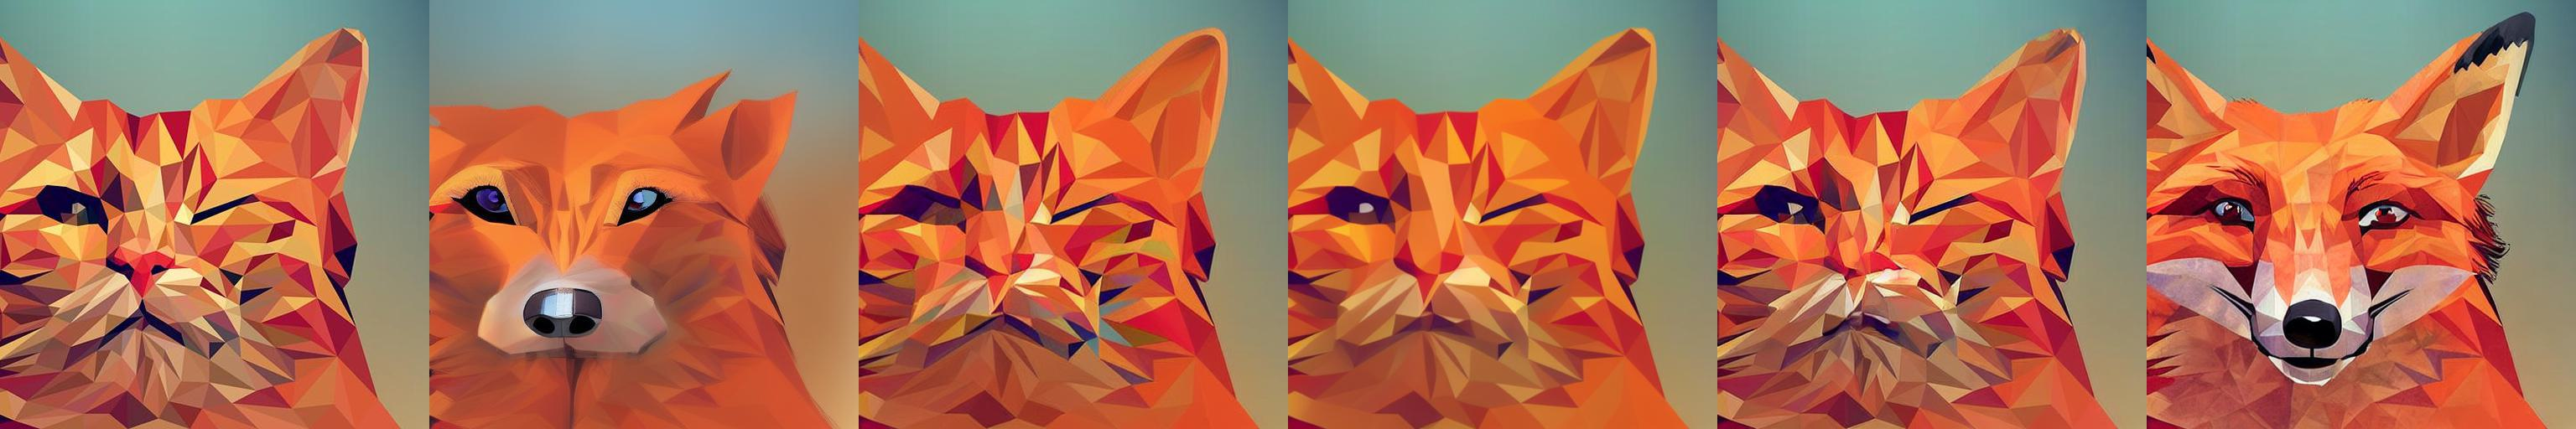
\includegraphics[width=\columnwidth]{fig/ex_all/0_random_140-000000000080}} \\
        \multicolumn{6}{c}{``\textit{a \textcolor{BrickRed}{\st{cat}} \textcolor{RoyalBlue}{\textbf{fox}} is shown in a low polygonal style}"} \\
        \multicolumn{6}{c}{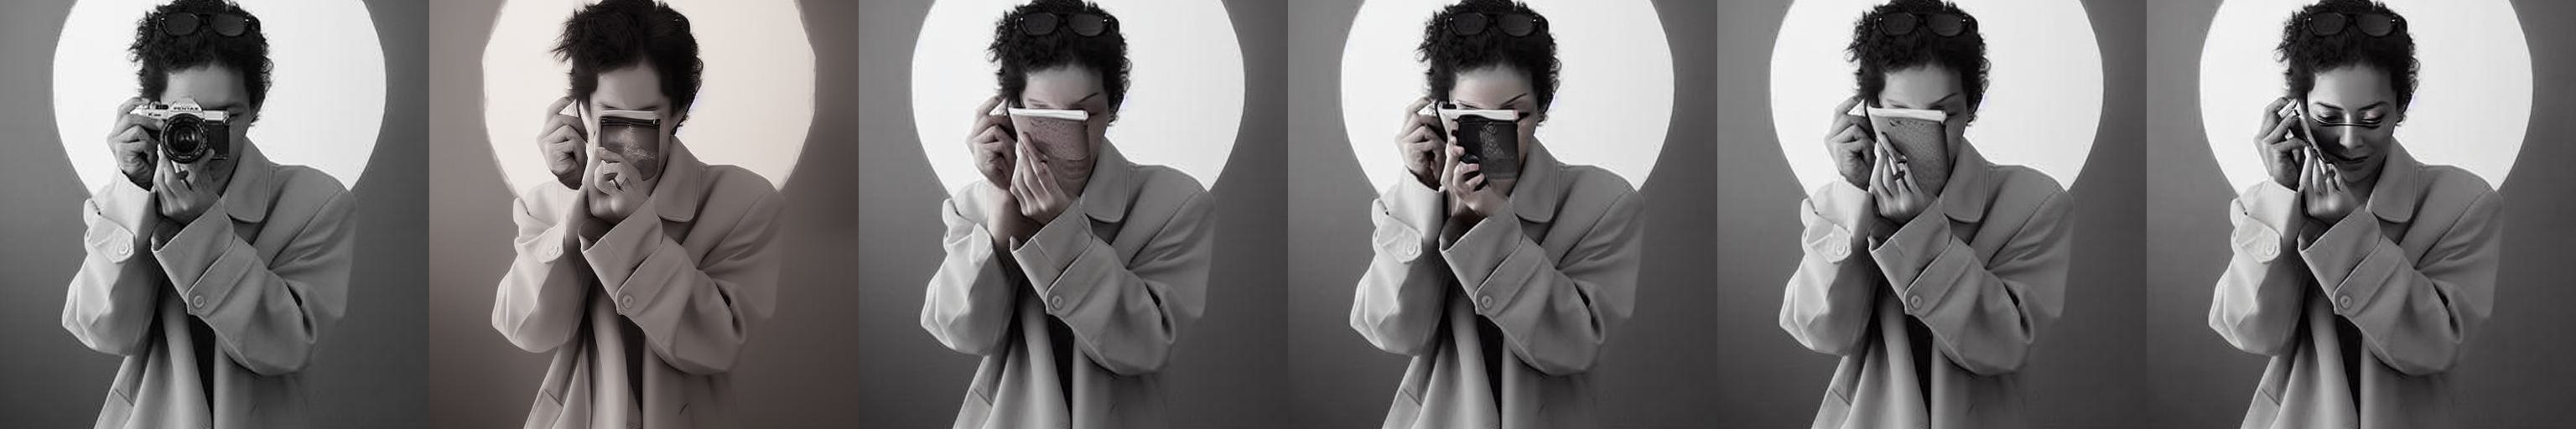
\includegraphics[width=\columnwidth]{fig/ex_all/1_change_object_80-2_natural-2_human-122000000002}} \\
        \multicolumn{6}{c}{``\textit{a woman in a coat holding a \textcolor{BrickRed}{\st{camera}} \textcolor{RoyalBlue}{\textbf{phone}} on white plate}"} \\
        \multicolumn{6}{c}{
\includegraphics[width=\columnwidth]{fig/ex_all/9_change_style_80-1_artificial-2_human-912000000001}} \\
        \multicolumn{6}{c}{``\textit{a clown \textcolor{RoyalBlue}{\textbf{in pixel art style}} with colorful hair}"} \\
        \multicolumn{6}{c}{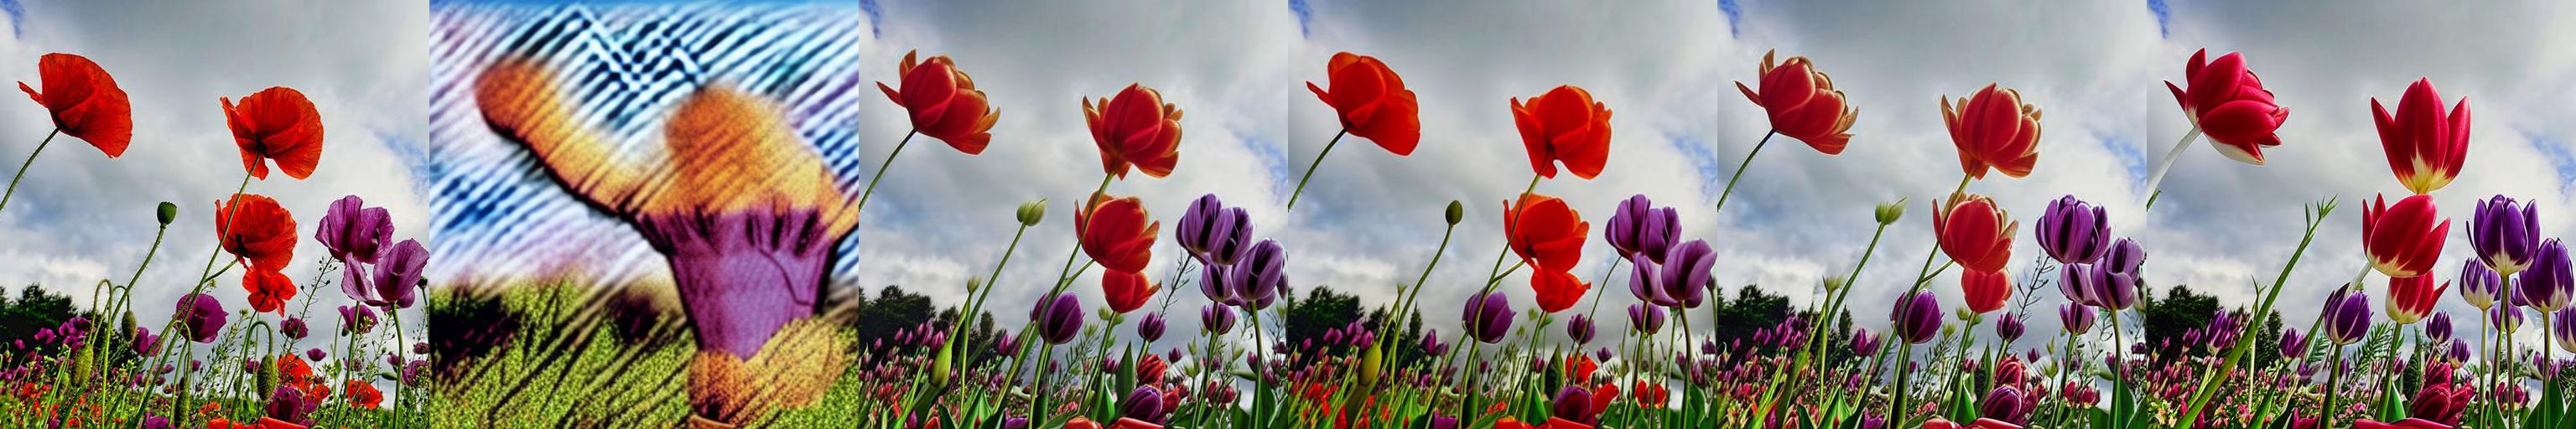
\includegraphics[width=\columnwidth]{fig/ex_all/0_random_140-000000000101}} \\
        \multicolumn{6}{c}{``\textit{\textcolor{BrickRed}{\st{poppies}} \textcolor{RoyalBlue}{\textbf{tulips}}}"} \\
        \multicolumn{6}{c}{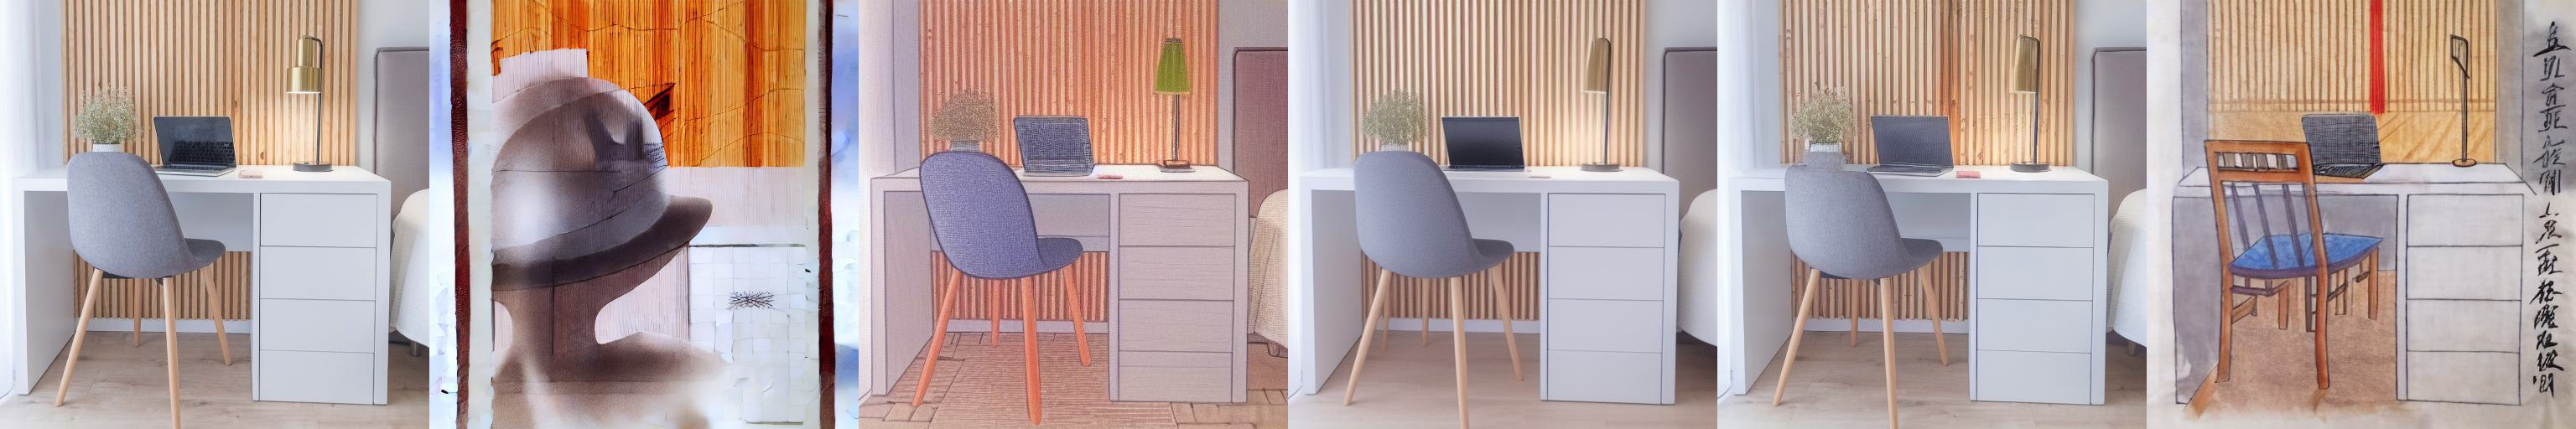
\includegraphics[width=\columnwidth]{fig/ex_all/9_change_style_80-2_natural-3_indoor-923000000007}} \\
        \multicolumn{6}{c}{``\textit{\textcolor{RoyalBlue}{\textbf{chinese painting of}} a white desk with a laptop and chair}"} \\
        \end{tabularx}
        \caption{Examples from the PieBench dataset illustrating the strengths of \method{}, including superior style transfer, content modification, and object removal.        }
    \label{fig:qual_adv}
  \end{figure}

{\modified{}The qualitative analysis in} Fig.~\ref{fig:method_comparison} is consistent with the quantitative evaluation. {\modified{}The proposed method} preserves the original image structure and content while still achieving good editing performance. For example, only \method{} and \negprox{} are able to preserve the appearance of the tree in the second row. Similarly, \method{} is the only method capable of preserving the details and colors of the t-shirt sleeve, hair, and background in the fourth row.


{\modified{}The proposed method also generates} more natural-looking images. This is especially noticeable in the dog and sushi examples. In the dog example, not only are the dog and the chair preserved, but also the dog's face and the illumination are more natural. In the sushi example, {\modified{}it} is the only method able to preserve all image details and color while generating a deeper red meat color as well as natural-looking \textit{nori} algae, whereas the rest generate shapeless and unnatural-looking sushi pieces. {\modified{}This result is attributed} to the fact that {\modified{}the presented} method is able to diminish the guidance term across time, as discussed in Sec~\ref{sec:self_attention_guidance}.


Furthermore, Fig.~\ref{fig:qual_adv} presents additional examples that showcase the unique strengths of \method{}, which are absent in the compared methods. Unlike these methods, {\modified{}the proposed approach} does not directly guide reconstruction in the $\vz$ latent space (additional experimentation in this regard can be found in supplementary materials' Sec. \ref{sec:sup_reconstruction}). Instead, it operates in the more abstract and semantically rich latent space of the attention layers. {\modified{}It is understood} that as the self-attention maps mostly encode low-resolution semantic features instead of shapes, SAGE is able to generate images that better capture the style while changing the content, has more freedom to edit the shape of elements (as the tulips in the fourth row), and is able to eliminate elements that are present in the original image while filling the gap with plausible content. Moreover, {\modified{}the proposed method} surpasses the compared approaches in transferring style from one image to another while simultaneously altering the content. Conversely, it can preserve content while significantly modifying the style. Notably, all of this is achieved without explicit reconstruction, marking a key distinction from existing methods.



\subsection{User Study}
\label{sec:userstudy}


To strengthen the comparison with existing approaches detailed in Sec.~\ref{sec:expsota}, {\modified{}a user study was conducted}. This study aimed to evaluate {\modified{}the proposed method} against others based on three key aspects: structure preservation, background preservation, and adherence to the prompt. Additionally, {\modified{}overall user preference was assessed}.

{\modified{}A total of 22 participants were recruited} to perform \textit{one-versus-one} comparisons between two randomly selected images from the PieBench \textit{random editing} task. The methods compared included \negativelong~\cite{miyake2023negative}, \directinversionlong~\cite{miyake2023negative}, \negproxlong~\cite{han2023proximal}, \ptopzerolong~\cite{parmar2023zero}, and {\modified{}the proposed method}. The results for most methods showed statistical significance without requiring further experimentation.

However, the comparison between \directinversion{} and \method{} resulted in a particularly tight margin. To ensure statistical significance in this case, an additional 25 participants were later asked to compare these two methods on the MagicBrush dataset, {\modified{}confirming} significance with a \textit{p-value} $< 0.01$ on all methods.


In the study, participants were provided with different sets of images depending on the evaluation criteria. For assessing structure preservation, they were shown the original image, together with two edited versions. In contrast, for background preservation evaluations, the input image was masked to highlight areas relevant to the task. When evaluating prompt fidelity and overall user preference, only the target prompt alongside the edited versions was displayed. Images were presented in a randomized sequence to ensure that participants focused on the relevant aspects for each criterion, and their judgments were unbiased, as they were not informed about which methods were used. 



{ 
    

\begin{table}[htbp]
    
    \small
    \centering
      \renewcommand\arraystretch{1.}
      \setlength{\tabcolsep}{0.7mm}{
    \begin{threeparttable}
    \begin{tabular}{ccccc}

    \toprule
    %\multicolumn{2}{c}{\textbf{Structure}}  &  \multicolumn{2}{c}{\textbf{Background}} & \multicolumn{2}{c}{\textbf{Prompt}} && \multicolumn{2}{c}{\textbf{Global}} \\ 
    \textbf{\method~vs}& \textbf{Structure\%}  &  \textbf{Background\%} & \textbf{Prompt\%} & \textbf{Global\%} \\
    \midrule
    % \ptopzerolong~\cite{parmar2023zero} & 93.8\% &	92.0\% &	83.0\% &	75.9\% \\
    % \nulltextlong~\cite{mokady2023null} & 70.5\% &	69.6\% &	52.7\% &	54.5\%  \\
    %  \directinversionlong~\cite{ju2023direct} & 55.4\% / 1 &	62.5\% &	52.7\% &	52.7\% \\
    %      \negproxlong~\cite{han2023proximal} & 58.9\% &	58.0\% &	62.5\% &	59.8\%  \\
    \ptopzero~\cite{parmar2023zero} &       93.8 &	            92.0 &	    83.0 &	    75.9 \\
    \nulltext~\cite{mokady2023null} &       70.5 &	            69.6 &	    52.7 &	    54.5  \\
     \directinversion~\cite{ju2023direct} & 55.4 / 52.0 &	    62.5 / 55.3 &	    52.7 / 46.5 &	    52.7 / 52.7 \\
         \negprox~\cite{han2023proximal} &  58.9 &	            58.0 &	    62.5 &	    59.8  \\
    % \midrule
    % Average & 69.6\% &	70.5\% &	62.7\% &	60.7\%  \\
    \bottomrule
    \end{tabular}
    % \begin{tablenotes}
    %    \footnotesize
    %    \item[a] Without cross-attention manipulation described in \ref{sec:cross_attention_manipulation}
    %    \item[b] Including cross-attention replacement
    %     \end{tablenotes}
    \end{threeparttable}
    }
        % \vspace{-0.2cm}
% \caption{User study results showing the frequency with which our method, \method, was preferred over the comparative methods. A total of 1792 questions were answered by participants. Additionally, \directinversion{} was evaluated in a separate user study involving 1540 questions on MagicBrush to assess statistical significance. All method comparisons demonstrate statistical significance with $p < 0.01$, determined using a binomial test and the \textit{Fisher} combined method.}

\caption{User study results showing the frequency with which {\modified{} the proposed method (\method{})} was preferred over {\modified{} compared methods}. A total of 1792 questions were answered by participants. For \directinversion{}, two results are reported: the first corresponds to the PieBench dataset{\modified{}}, consistent with other methods, while the second represents the user study conducted on MagicBrush with 1540 additional questions to assess statistical significance. All method comparisons demonstrate statistical significance with $p < 0.01$, determined using a binomial test and the \textit{Fisher} method for {\modified{}combining} \textit{p-values}.}



            \label{tab:user_study}
        % \vspace{-0.2cm}
    \end{table}

    
    
    
    }
    

The results of these evaluations are compiled in Table~\ref{tab:user_study}. They corroborate {\modified{}the quantitative evaluations}, demonstrating a consistent preference for {\modified{}the proposed method} across all four evaluation criteria. While the preference margin for {\modified{}the method} is somewhat narrow when compared to Direct Inversion in aspects like prompt fidelity and overall preference, a significant difference is observed in terms of background preservation. This pronounced advantage in preserving the background further highlights the effectiveness of {\modified{}the presented approach}. Overall, the user study solidifies the robust performance of {\modified{}the method}, highlighted by the global preference, supporting its strengths not only in quantitative metrics but also in subjective user assessments.
 
\subsection{Limitations}
\label{sec:limitations}


The main limitation of \method{}, as {\modified{}with} other diffusion-based editing methods \cite{han2023proximal}, is its hyperparameter sensitivity. Adjusting hyperparameters for each image enhances quality but affects user experience, making it hard to standardize a single parameter set for diverse editing tasks. {\modified{}Specific failure cases} of \method{} are discussed in the supplementary materials.


% \newpage
\section{Conclusions}

{\modified{}This work revisited} the conventional approach to prompt-based image editing within diffusion models. Contrary to established methods that leverage both negative and positive branches of Classifier-Free Guidance for editing ($\pin$ and $\pout$, respectively), {\modified{}the presented investigation reveals} that reconstruction is not necessary. {\modified{}The DDIM inversion process alone contains} enough information for effective editing, thereby questioning the need for manipulating $\pin$ and $\pout$ attention maps. {\modified{}The proposed approach simplifies} the editing process by applying guidance exclusively to the $\pin$ branch, which not only streamlines the method but also yields better results, as confirmed by extensive comparative analyses.


{\modified{}The primary contribution lies} in introducing and validating self-attention guidance as a superior mechanism for image editing tasks. Through quantitative analyses, ablation studies, and user feedback, {\modified{}it was demonstrated} that self-attention guidance captures a broader contextual understanding, enabling better edits compared to traditional cross-attention techniques. This approach preserves closer fidelity to the original image content while accurately applying the desired edits. 

{\modified{}A comprehensive comparative analysis}, supported by an extensive user study, shows that SAGE is preferred over every other compared method with statistical significance (\textit{p-value} $< 0.01$), achieving an average preference higher than 60.7\% among participants. This substantial margin underscores SAGE's effectiveness and potential to redefine standard practices in image editing with diffusion models.

% {\modified{}Several key areas} for improvement and future research {\modified{}have been identified}. For object removal, masking out self-attention guidance could prevent structure preservation in emptied areas, addressing issues in Sec.~\ref{sec:sup_limitations_structure} of the supplementary materials.
% {\modified{}Further exploration of sampling schedulers beyond DDIM and applying SAGE to distilled models \cite{meng2023distillation} and rectified-flow models \cite{liu2023flow} could benefit performance, taking advantage of more stable inference trajectoriesand higher quality models \cite{deng2024fireflow}}.
% Additionally, minimizing reliance on precise hyperparameter tuning by dynamically adjusting parameters based on task complexity, input characteristics, and denoising magnitude could enhance robustness across diverse editing scenarios.


{\modified{}Several directions for improvement and future research have been identified. For object removal, masking out self-attention guidance could mitigate unintended structure preservation. Investigating alternative sampling schedulers beyond DDIM and extending SAGE to higher-quality models, such as distilled models~\cite{meng2023distillation} or rectified-flow models~\cite{liu2023flow,deng2024fireflow}, may further enhance results while reducing the number of sampling steps required. Additionally, dynamically adapting hyperparameters based on task complexity, input characteristics, and denoising magnitude could improve robustness across a wide range of editing scenarios.}

\section*{Acknowledgements}
\label{sec:acknowledgements}

This work was supported by the Spanish Ministry of Science, Innovation, and Universities (MICIU) under grant FPU19/00591, grant CONFIA (PID2021-122916NB-I00) funded by MICIU/AEI/10.13039/501100011033 and by “ERDF A way of making Europe” and by the French National Research Agency (ANR- 20-CE23-0027).

% {
%     \small
%     \bibliographystyle{ieeenat_fullname}
%     \bibliography{main}
% }

\bibliographystyle{IEEEtran}
\bibliography{main}

% \input{sec/8_bio}

% WARNING: do not forget to delete the supplementary pages from your submission 
\clearpage
\setcounter{page}{1}
\maketitlesupplementary


% The supplementary materials provide additional analysis to enrich the main paper, along with further results and insights.
% This document is organized as follows: In Section~\ref{sec:sup_sourcecode} we provide the source code and demo resources, with implementation details in Section~\ref{sec:sup_sourcecode_details}. Section~\ref{sec:sup_results} presents additional results, including a time and memory analysis (Section~\ref{sec:sup_results_time}), guidance ablations (Section~\ref{sub:sup_results_ablation}), and a reconstruction evaluation (Section~\ref{sec:sup_reconstruction}). Finally, Sections~\ref{sec:sup_limitations_structure} and~\ref{sec:sup_limitations_failure} discuss limitations regarding structure preservation and failure cases.


The supplementary materials provide additional analysis to enrich the main paper, along with further results and insights. This document is structured as follows: Section~\ref{sec:sup_sourcecode} contains the source code and demo resources, with implementation information provided in Section~\ref{sec:sup_sourcecode_details}. Section~\ref{sec:sup_results} presents additional experimental outcomes including time and memory requirements (Section~\ref{sec:sup_results_time}), guidance ablations (Section~\ref{sub:sup_results_ablation}), and an evaluation of reconstruction performance (Section~\ref{sec:sup_reconstruction}). Finally, Sections~\ref{sec:sup_limitations_structure} and~\ref{sec:sup_limitations_failure} discuss limitations regarding structure preservation and failure cases.









\section{Source Code}
\label{sec:sup_sourcecode}
% The source code, the scripts to replicate the experiments, as well as a web demo both off-line (\textit{i.e.,} the Gradio app) and on-line (\textit{i.e.,} Huggingface demo) are available at \codeurl{}.The PIE-Bench images corresponding to the quantitative results in Tables \ref{tab:ablation_piebench}, \ref{tab:comparison_piebench}, and \ref{tab:user_study} of the main paper are available as well in a PNG file with all the parameters as metadata so further analysis can be performed on it if needed.

The source code, scripts for replicating the experiments, and a web demo (including an offline version via the Gradio app and an online version hosted on Hugging Face) are available at \codeurl{}. Additionally, the PIE-Bench and MagicBrush images used for the quantitative results in Tables \ref{tab:ablation_piebench}, \ref{tab:comparison_piebench}, and \ref{tab:user_study} of the main paper are also accessible. These images are provided in PNG format, with all editing parameters embedded as metadata, facilitating further independent analysis.

\subsection{Implementation Details}
\label{sec:sup_sourcecode_details}

In our preliminary analysis, best results for $512 \times 512$ images were achieved with $32 \times 32$ self-attention maps and $16 \times 16$ cross-attention maps, particularly from the second and third encoder blocks of the U-Net respectively and the corresponding upsampling block, similar to \cite{hertz2023prompt}. For $ 768 \times 768 $ images, the best results were obtained with $ 24 \times 24 $ self-attention and cross-attention maps, specifically from the third block. Additionally, our code supports FP16 computation, including gradient calculation, which significantly reduces time and memory consumption. To prevent gradients from becoming zero in half-precision floating-point arithmetic, the loss term is scaled by a factor of 500 prior to gradient computation, with the weighting factor $\lambda$ applied afterward (Sec.~\ref{sec:self_attention_guidance}).



\section{Additional Results}
\label{sec:sup_results}

\subsection{Inference time and memory comparison}
\label{sec:sup_results_time}

% \begin{table*}[htbp]
%     \centering
%       \renewcommand\arraystretch{0.9}
%       \setlength{\tabcolsep}{0.3mm}{
%     \begin{threeparttable}
%     \begin{tabular}{c|c|cccc|cc}
%     \toprule
%     \toprule
%           & \textbf{Structure}          & \multicolumn{4}{c|}{\textbf{Background Preservation}} & \multicolumn{2}{c}{\textbf{CLIP Similariy}} \\ \midrule
%     \textbf{Method}            & \textbf{Distance}$_{^{\times 10^3}}$ $\downarrow$ & \textbf{PSNR} $\uparrow$     & \textbf{LPIPS}$_{^{\times 10^3}}$ $\downarrow$  & \textbf{MSE}$_{^{\times 10^4}}$ $\downarrow$     & \textbf{SSIM}$_{^{\times 10^2}}$ $\uparrow$    & \textbf{Whole}  $\uparrow$          & \textbf{Edited}  $\uparrow$       \\ \midrule
%     \textbf{Null-text} \cite{mokady2023null} & 13.44           & 27.03  & 60.67  & 35.86  & 84.11 & 24.75        & 21.86          \\
%     \textbf{Negative prompt} \cite{miyake2023negative} &     16.17       &  26.21 &  69.01  &  39.73 & 83.40 &   24.61     &    21.87     \\
%     \textbf{Direct inversion} \cite{ju2023direct} & 11.65           & 27.22  & 54.55  & 32.86  & 84.76 & 25.02         & \textbf{22.10}          \\
%     \textbf{P2P-Zero} \cite{parmar2023zero} & 61.68 & 20.44  & 172.22 & 144.12 & 74.67 & 22.80 & 20.54 \\
%     \textbf{Plug-n-Play} \cite{tumanyan2023plug} \tnote{a} & 28.22 & 22.28  & 113.46 & 83.64 & 79.05 & 25.41 & 22.55 \\
%     \textbf{NegProx} \cite{miyake2023negative} \tnote{b} & \textbf{7.44} & \textbf{28.67} &	41.98 &	\textbf{24.25} &	\textbf{85.98} &	24.28 &	21.36 \\
%     % \textbf{Ours} (temporal) & 24.21 &	25.53 &	62.64 &	55.27 &	83.97 &	\textbf{26.18} &	\textbf{22.86} \\
%     \textbf{Ours} & 10.96 &	27.91 &	\textbf{39.56} &	29.80 &	85.97 &	\textbf{25.47} &	21.96 \\
%     \textbf{Ours} (by task) & 12.70 &	27.67 &	42.30 &	32.09 &	85.71 &	25.75 &	22.37 \\
    
%     \bottomrule
%     \bottomrule
%     \end{tabular}
%     \begin{tablenotes}
%        \footnotesize
%        \item[a] use Stable Diffusion v1.5 as base model (others all use Stable Diffusion v1.4) %revise the source code's 1000 steps to 50 steps
%        \item[b] Proximal guidance with negative prompt as introduced in \cite{han2023proximal}
%         \end{tablenotes}
%     \end{threeparttable}
%     }
%         \vspace{-0.2cm}
%     \caption{Quantitutive analysis performed on PieBench \cite{ju2023direct}. All rows but ours are taken from \cite{ju2023direct}.}
%             \label{tab:comparison_piebench}
%         \vspace{-0.2cm}
%     \end{table*}
    

% \begin{table*}[htbp]
%     \centering
%     \small
%       \renewcommand\arraystretch{0.9}
%       \setlength{\tabcolsep}{0.3mm}{
%     \begin{threeparttable}
%     \begin{tabular}{cccccc}
%    % \toprule
%     \toprule
%           & \textbf{Struct.}          & \multicolumn{2}{c|}{\textbf{Background Preservation}} & \multicolumn{2}{c}{\textbf{CLIP Similariy}} \\ \midrule
%     \textbf{Method}            & \textbf{Distance}$_{^{\times 10^3}}$ $\downarrow$ &   \textbf{LPIPS}$_{^{\times 10^3}}$ $\downarrow$  & \textbf{SSIM}$_{^{\times 10^2}}$ $\uparrow$    & \textbf{Whole}  $\uparrow$          & \textbf{Edited}  $\uparrow$       \\ \midrule
%     \textbf{\nulltextlong} \cite{mokady2023null} & 13.4             & 60.7    & 84.1 & 24.8        & 21.9          \\
%     \textbf{Negative prompt} \cite{miyake2023negative} &     16.2        &  69.0   & 83.4 &   24.6     &    21.9     \\
%     \textbf{\directinversionlong} \cite{ju2023direct} & 11.7             & 54.6    & 84.8 & 25.0         & 22.1          \\
%     \textbf{\ptopzerolong} \cite{parmar2023zero} & 61.7   & 172.2 & 74.7 & 22.8 & 20.5 \\
%     \textbf{\pnplong} \cite{tumanyan2023plug} \tnote{a} & 28.2   & 113.5 & 79.0 & 25.4 & \textbf{22.6} \\
%     \textbf{\negproxlong} \cite{miyake2023negative} \tnote{b} & \textbf{7.4}  &	42.0  &	\textbf{86.0} &	24.3 &	21.4 \\
%     % \textbf{Ours} (temporal) & 24.21 &	25.53 &	62.64 &	55.27 &	83.97 &	\textbf{26.18} &	\textbf{22.86} \\
%     \textbf{\method} (ours) & 11.0 &	\textbf{39.6} &	\textbf{86.0} &	\textbf{25.5} &	22.0 \\
%     % \textbf{Ours} (by task) & 12.70 &	42.30  &	85.71 &	25.75 &	22.37 \\
    
%     \bottomrule
%     %\bottomrule
%     \end{tabular}
%     \begin{tablenotes}
%        \footnotesize
%        \item[a] use Stable Diffusion v1.5 as base model (others all use Stable Diffusion v1.4) %revise the source code's 1000 steps to 50 steps
%        \item[b] Proximal guidance with negative prompt as introduced in \cite{han2023proximal}
%         \end{tablenotes}
%     \end{threeparttable}
%     }
%         \vspace{-0.2cm}
%     \caption{Quantitative analysis performed on PieBench \cite{ju2023direct}. All rows but ours are taken from \cite{ju2023direct}.}
%             \label{tab:comparison_piebench}
%         \vspace{-0.2cm}
%     \end{table*}




    \begin{table}[htbp]
    \centering
    \small
      \renewcommand\arraystretch{0.5}
      \setlength{\tabcolsep}{0.5mm}{
  \resizebox{0.9\linewidth}{!}{ 
%   \begin{threeparttable}  
  \begin{tabular}{ccc}
   % \toprule
    \toprule
    \textbf{Method}             &   \textbf{Time} (s)  $\downarrow$  & \textbf{Memory} (GB) $\downarrow$\\ \midrule
    
    % \textbf{\nulltextlong} \cite{mokady2023null} & 115.28	& 21.08\\
    % \textbf{Negative prompt} \cite{miyake2023negative} & 26.58	& 38.90\\
    % \textbf{\negproxlong} \cite{miyake2023negative}  & 23.89 &	38.90 \\
    % \textbf{\pnplong} \cite{tumanyan2023plug}  & \textbf{12.53}	& 38.89 \\
    % \textbf{\directinversionlong} \cite{ju2023direct} & 33.40	& \textbf{12.43} \\
    % \textbf{\directinversionlong} \textit{FP16} \cite{ju2023direct} & 12.50	& \textbf{7.38} \\
    % \textbf{\ptopzerolong} \cite{parmar2023zero} & 52.66 &	24.97\\
    % \textbf{\method} (ours) & 12.64* & 7.41* \\
    % \textbf{\method} \textit{FP32} (ours) & 79.63 &	29.31 \\
    
    \nulltextlong{} \cite{mokady2023null} & 115.3	& 21.1\\
    Negative prompt \cite{miyake2023negative} & 26.6	& 38.9\\
    \negproxlong{} \cite{miyake2023negative}  & 23.9 &	38.9 \\
    \textbf{\pnplong{}} \cite{tumanyan2023plug}  & \textbf{12.5}*	& 38.9 \\
    \textbf{\directinversionlong{}} \cite{ju2023direct} & 33.4	& \textbf{12.4}* \\
    \textbf{\directinversionlong{}} \textit{FP16} \cite{ju2023direct} & \textbf{12.5}	& \textbf{7.4} \\
    \ptopzerolong \cite{parmar2023zero} & 52.7 &	25.0\\
    \textbf{\method{}} (ours) & 12.6 & \textbf{7.4} \\
    \method{} \textit{FP32} (ours) & 27.6 &	29.3 \\
    
    \bottomrule
    %\bottomrule
    \end{tabular}
    % \begin{tablenotes}
    %     \item[*] SAGE is the only method design to work explicitly on 16-bit precision.
    % \end{tablenotes}
    % \end{threeparttable}
    }

    }
        % \vspace{-0.2cm}
    \caption{
        % Performance comparison for both time and memory consumption run on a NVIDIA A100-40GB. The results described in the Time column correspond to the time required to generate two images of size $512\times512$ pixels minus the time required to generate only one image. This way we can isolate the time required to generate an image without the overhead of loading the model and the data. The results described in the Memory column correspond to the maximum allocated memory for a single image generation as reported by \texttt{nvidia-smi}.\\
        % The best results for FP32 precision methods are marked with *.
        Performance of prompt-based editing methods on a NVIDIA A100-40GB GPU. The Time column reflects extra time to generate a second 512×512 image (isolating generation cost), and the Memory column shows the peak memory usage per image. FP32 best results are marked with *.
}
            \label{tab:comparison_time}
        % \vspace{-0.2cm}
    \end{table}


  

% \begin{figure}
%     \centering
%     \includegraphics[width=0.99\linewidth]{fig/time.pdf}
%     \caption{Running time required to generate\steph{edit?} 1, 2, and 5 images sequentially. For \method{} we describe two experimental settings, with 16FP and 32FP precision, named \textit{\method} and \textit{\method{} (FP32)} respectively.}
%     \label{fig:comparison_time}
% \end{figure}

% In Table \ref{tab:comparison_time} we show that the FP16 version of \method{} has the smallest memory footprint among the compared methods and it is also the second fastest method by a tenth of a second. Meanwhile the FP32 version is still competitive with the other three best methods. The results for \nulltext{}, \pnp{}, \ptopzero, and \directinversion{} are obtained with \directinversion{}'s \cite{ju2023direct} source code \footnote{\url{https://github.com/cure-lab/DirectInversion}}, the results for \negative{} and \negprox{} are based on the source code from \cite{han2023proximal} \footnote{\url{https://github.com/phymhan/prompt-to-prompt}}. Every code is executed in the same conda environment on a NVIDIA A100-40GB GPU.

% The underlying reasons for \method{}'s competitive performance in both processing speed and memory efficiency, despite employing a computationally intensive operation such as gradient-based guidance, are twofold. Primarily, the computation of guidance is limited to a subset of self-attention maps, significantly reducing the overall computational load. Secondly, and perhaps most notably, \method{} distinguishes itself from the remaining methods evaluated by omitting the input image reconstruction step entirely. This strategic omission not only streamlines the process, enhancing efficiency, but also contributes to the method's reduced memory usage. These innovations collectively underscore \method{}'s ability to deliver high performance while navigating the challenges of resource constraints.


Table~\ref{tab:comparison_time} summarizes the performance of various prompt-based editing methods on a NVIDIA A100-40GB GPU. The Time column reports the additional time required to generate a second 512×512 image (isolating generation cost from model/data loading), and the Memory column indicates the peak memory allocated per image as measured using the command-line utility \texttt{nvidia-smi}.

Our FP16 version of \method{} uses the least memory (7.4 GB) and is the second fastest (12.6 s), while the FP32 version also remains competitive. These advantages are primarily due to two factors: (i) gradient-based guidance is computed on only a subset of self-attention maps, greatly reducing computational load, and (ii) the complete omission of the input image reconstruction step streamlines processing and lowers memory usage. All methods were executed under identical conditions using their original codebases.


\begin{figure}[h]
    \centering
    \begin{tabular}{m{1.5cm}m{1.5cm}m{1.5cm}m{0.4cm}m{0.5cm}}
    %   \hline

    %   \multirow{2}{*}{Input} &  (i) & (ii) & (iii) & (iv) & (v) & (vi) \\
    %   &  CA guidance &  $\vz_t$  guidance & SA replace.&  SA guidance &   (iv)+CA replace. &  (v) + LB \\
      %& \centering  CA guidance & \centering  $\vz_t$  guidance & \centering  SA replace.& \centering : SA guidance & \centering  (iv)+CA replace. & \centering  (v) + LB \\
    %   \hline
    %   \multicolumn{7}{c}{``\textit{a girl with blonde hair \textcolor{RoyalBlue}{\textbf{and a fluffy rainbow hat}} smiling}"} \\
    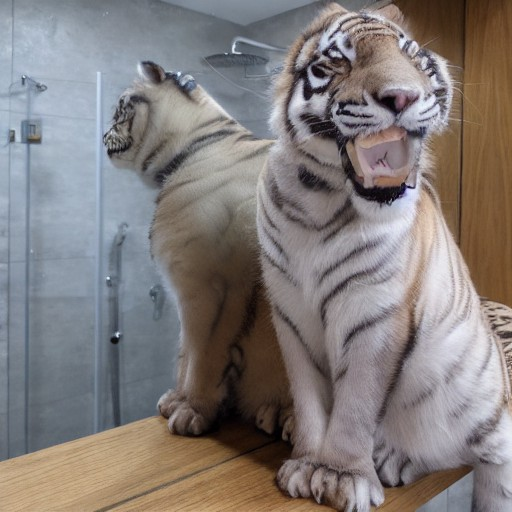
\includegraphics[width=1.5cm]{fig/cfg_self_matrix/m_2_50} & 
\includegraphics[width=1.5cm]{fig/cfg_self_matrix/m_2_250} & 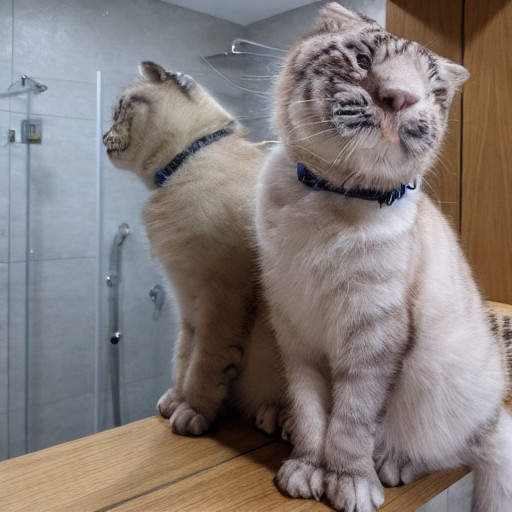
\includegraphics[width=1.5cm]{fig/cfg_self_matrix/m_2_500} & \rotatebox[origin=c]{90}{$w=2$} & \multirow{3}{*}{\rotatebox[origin=c]{90}{\textit{Classifier-Free guidance}}} \\
    
    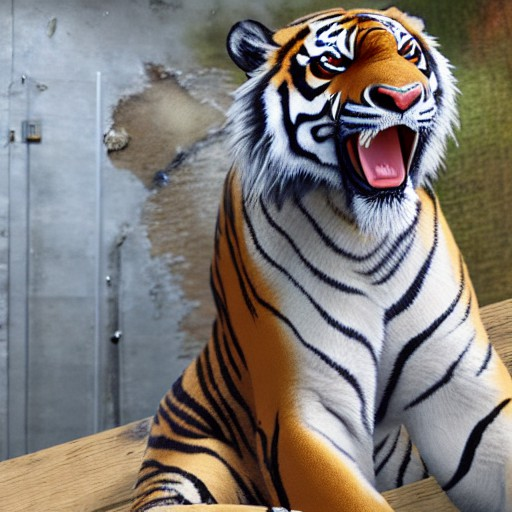
\includegraphics[width=1.5cm]{fig/cfg_self_matrix/m_75_50} & 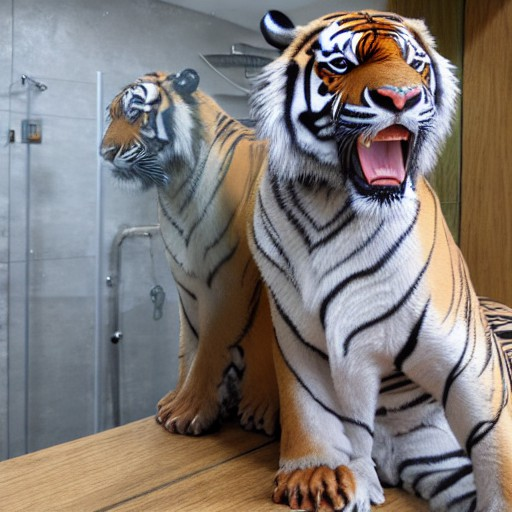
\includegraphics[width=1.5cm]{fig/cfg_self_matrix/m_75_250} & 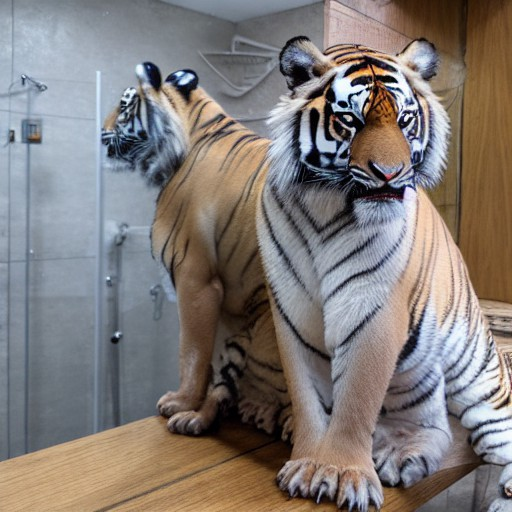
\includegraphics[width=1.5cm]{fig/cfg_self_matrix/m_75_500} & \rotatebox[origin=c]{90}{$w=7.5$} &  \\
    %   \multicolumn{7}{c}{``\textit{a baby with a stuffed \textcolor{BrickRed}{\st{monkey}} \textcolor{RoyalBlue}{\textbf{zebra}} in a car}"} \\
    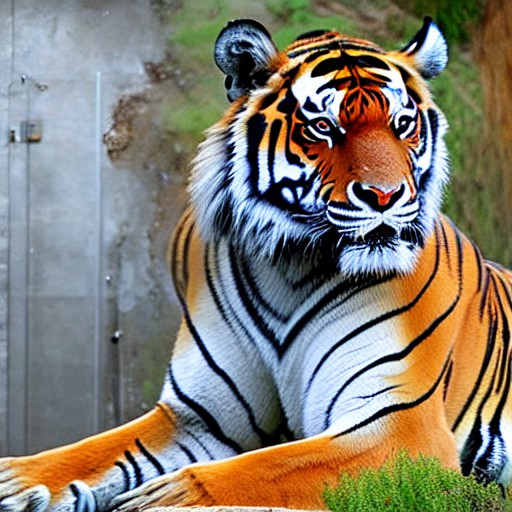
\includegraphics[width=1.5cm]{fig/cfg_self_matrix/m_15_50} & 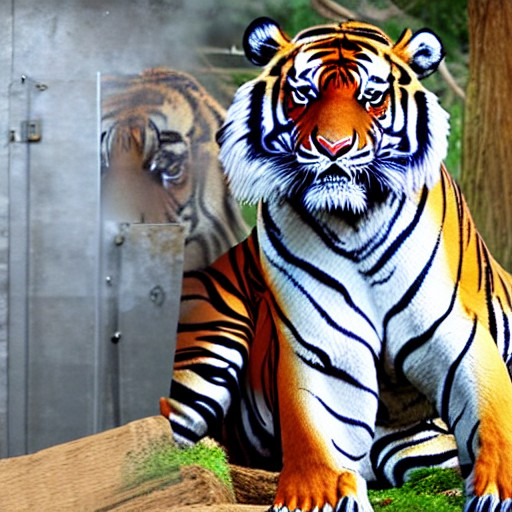
\includegraphics[width=1.5cm]{fig/cfg_self_matrix/m_15_250} & 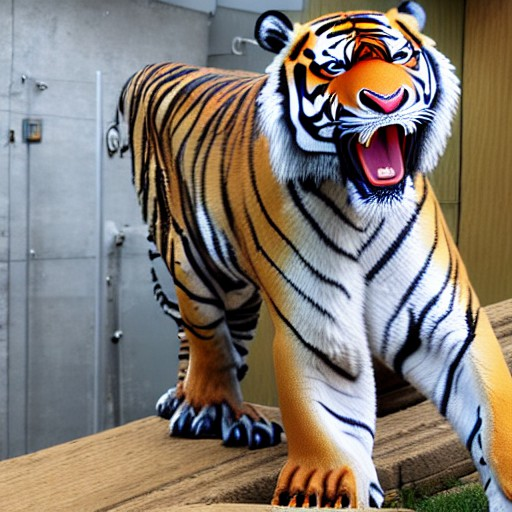
\includegraphics[width=1.5cm]{fig/cfg_self_matrix/m_15_500} & \rotatebox[origin=c]{90}{$w=15$} &  \\
    \centering  $ \lambda = 50 $  & \centering  $ \lambda = 250 $ & \centering  $ \lambda = 500 $ & & \\
    \multicolumn{3}{c}{\textit{Self-attention guidance}} & & \\
      % ... Add more rows as needed
    \end{tabular}
    % \caption{Matrix showing CFG $w$ and self-attention guidance scale $\lambda$ and how each of them drives the image generation toward reconstruction (high $\lambda$ and low $w$) or editing (low $\lambda$ and high $w$). Prompt: ``\textit{a \textcolor{BrickRed}{\st{cat}} \textcolor{RoyalBlue}{\textbf{tiger}} sitting next to a mirror}"}
    \caption{This matrix illustrates the interplay between CFG $w$ and self-attention guidance scale $\lambda$, highlighting their influence on image generation. The matrix shows how varying levels of $\lambda$ and $w$ drive the generated image toward either reconstruction (achieved with high $\lambda$ and low $w$) or editing (achieved with low $\lambda$ and high $w$). The images are generated based on the prompt ``'\textit{a \textcolor{BrickRed}{\st{cat}} \textcolor{RoyalBlue}{\textbf{tiger}} sitting next to a mirror}''.}
    \label{fig:supablation_cfg_guidance}
  \end{figure}

\subsection{Classifier-Free and Self-attention guidance} 

\label{sub:sup_results_ablation}

Figure~\ref{fig:supablation_cfg_guidance} evaluates the impact of both classifier-free guidance ($w$) and self-attention guidance ($\lambda$) on the generation process. It can be seen how a higher $\lambda$ value results in greater attention to the input structure, whereas greater $w$ values result in more plausible generation but also in more saturated colors (already discussed in \cite{ho2021classifier}). Higher self-attention guidance $\lambda$ values result in both better structure preservation and better color preservation as it reduces the negative impact of high CFG in natural looking colors. An appropiate balance is necessary to generate images that preserve the structure of the input image while performing deep, natural-looking transformations that reflect $\pout$.


\setlength{\tabcolsep}{1pt}
\begin{figure}[h]
    \footnotesize
    \small
    \centering
    % \begin{tabular}{*{6}{p{2.8cm}}}
    %   \hline
    %   & & & & & \\
    %   \centering Input & \centering \ptopzero & \centering \nulltext & \centering  \directinversion & \centering  \negprox & \centering \method{} \\
    %   %   \multicolumn{6}{c}{``\textit{A \textcolor{RoyalBlue}{\textbf{lego}} cat \textcolor{RoyalBlue}{\textbf{toy}} sitting next to a mirror}"} \\
    %   \multicolumn{6}{c}{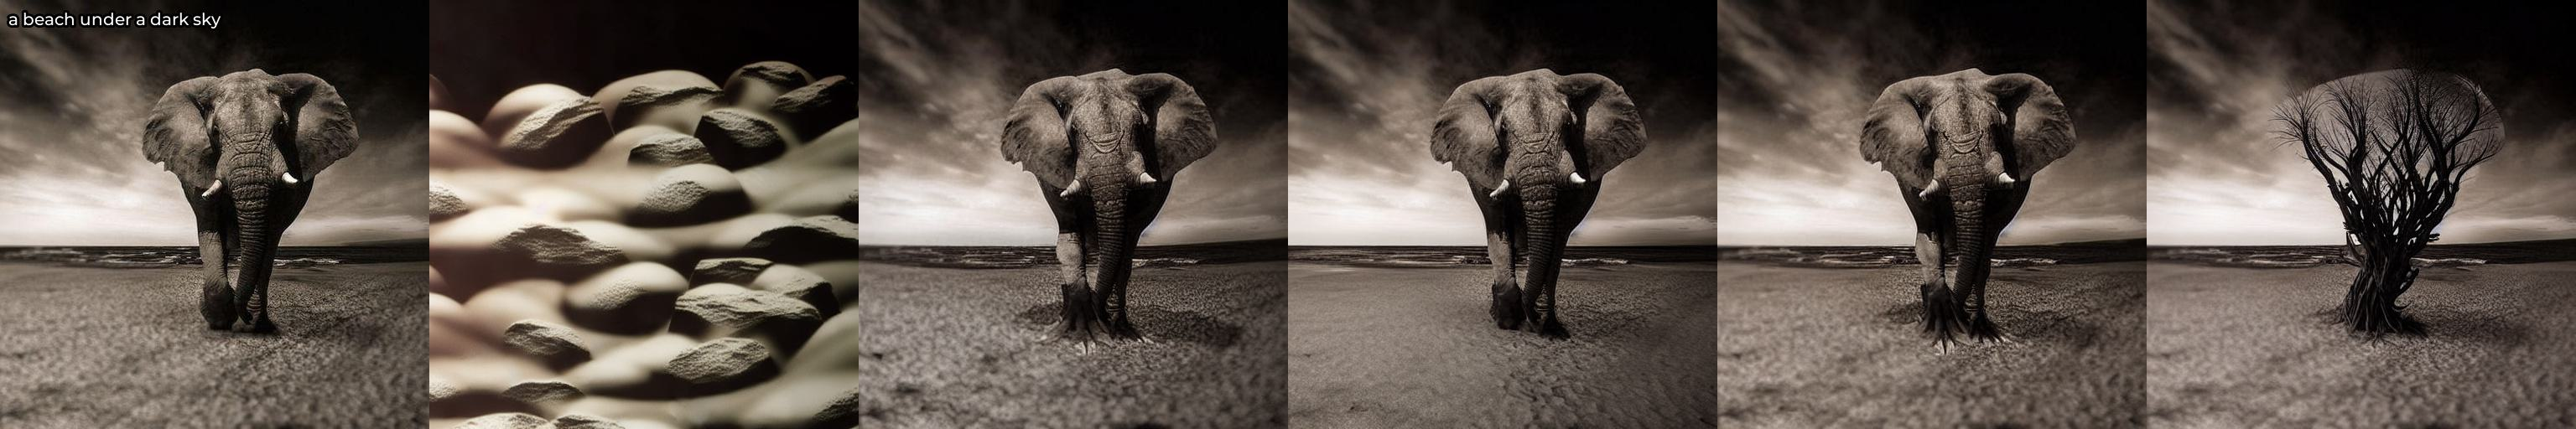
\includegraphics[width=\linewidth]{fig/ex_structpres/3_delete_object_80-2_natural-1_animal-321000000005}} \\
    % \multicolumn{6}{c}{}  \\
    % % 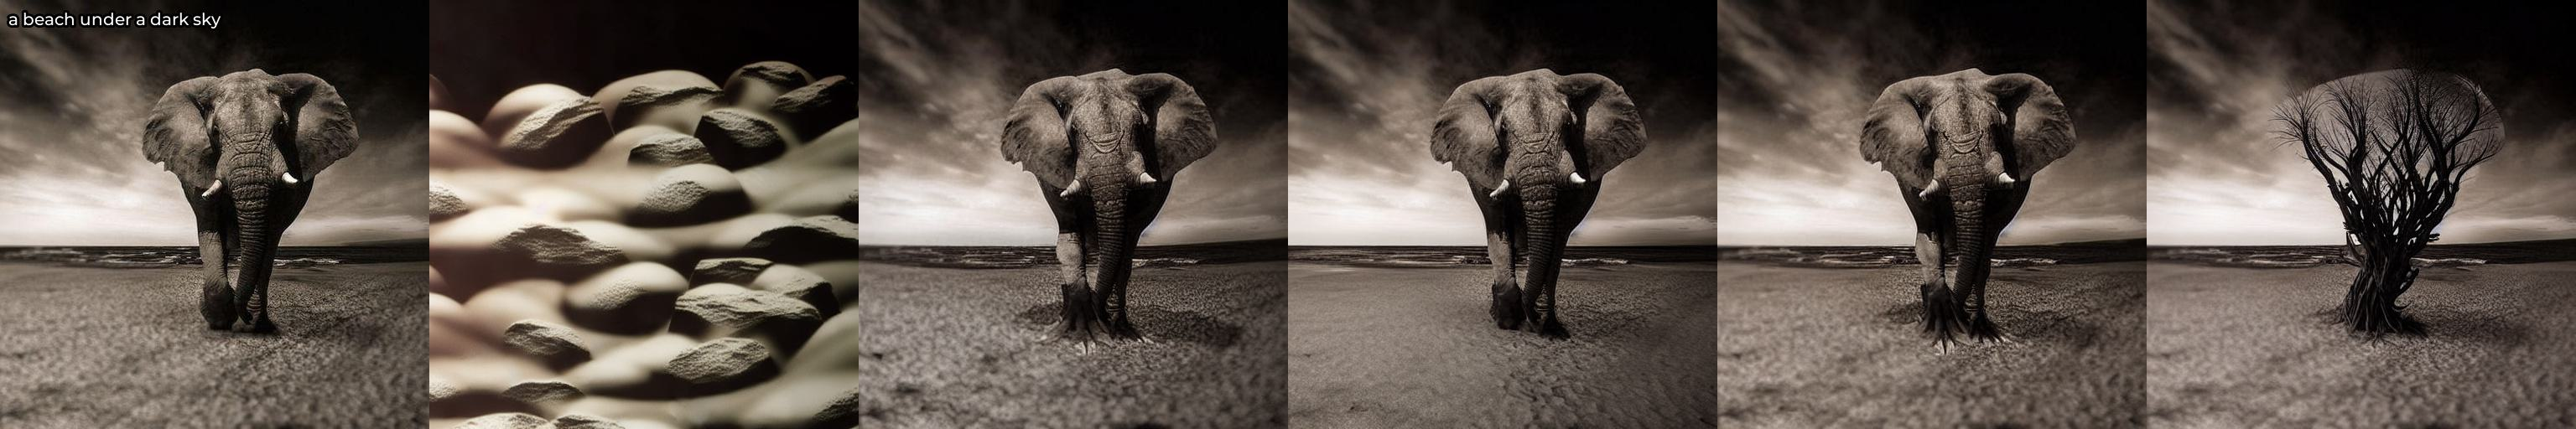
\includegraphics[height=2.2cm]{fig/ex_structpres/3_delete_object_80-2_natural-1_animal-321000000005} \\
    % %   \multicolumn{6}{c}{``\textit{Orange van with \textcolor{BrickRed}{\st{surfboards}} \textcolor{RoyalBlue}{\textbf{flowers}} on top}"} \\
    % %   \insertimage{van}{input}\\
    % %   \multicolumn{6}{c}{``\textit{Meat \textcolor{BrickRed}{\st{balls}} \textcolor{RoyalBlue}{\textbf{shushi}} on white plate}"} \\
    % %   \insertimage{meat}{input}\\
    % %   \multicolumn{6}{c}{``\textit{A \textcolor{BrickRed}{\st{woman}} \textcolor{RoyalBlue}{\textbf{storm-trooper}} with blue hair}"} \\
    % %   \insertimage{girl}{input}\\
    % %   \multicolumn{6}{c}{``\textit{A \textcolor{BrickRed}{\st{cat}} \textcolor{RoyalBlue}{\textbf{dog}} sitting on a wooden chair}"} \\
    % %   \insertimage{cat2}{input}\\
    %   \hline
    %   % ... Add more rows as needed
    % \end{tabular}
    \begin{tabularx}{0.7\columnwidth}{ YYYY }
        VAE & \method &  VAE & \method  \\
        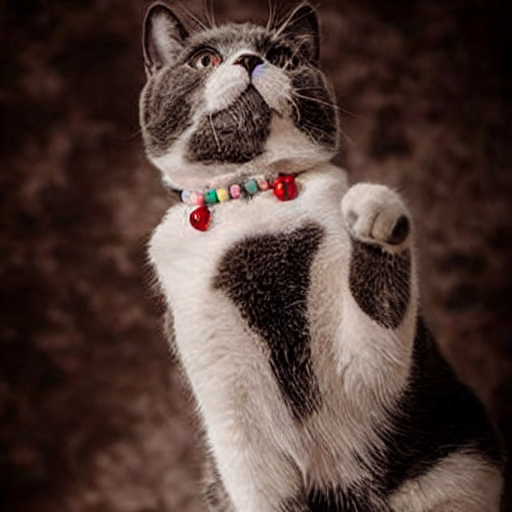
\includegraphics[width=\linewidth]{fig/reconstruction/000000000040_vae.png} & 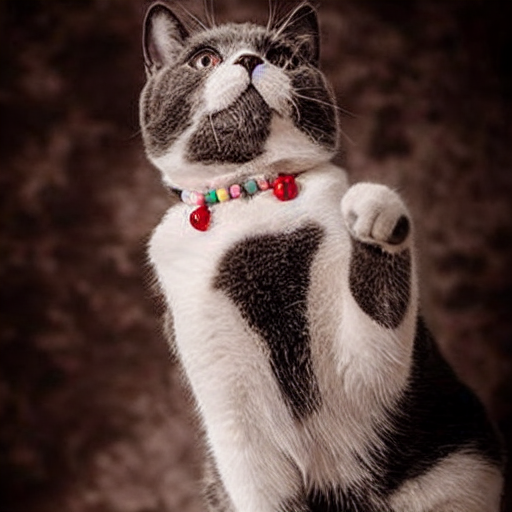
\includegraphics[width=\linewidth]{fig/reconstruction/000000000040.png} &
        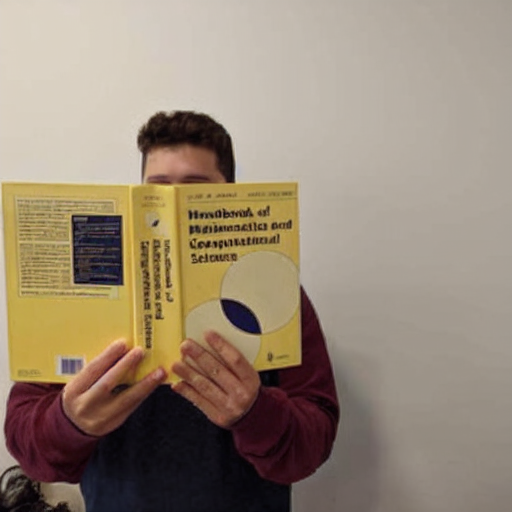
\includegraphics[width=\linewidth]{fig/reconstruction/223000000000_vae.png} & 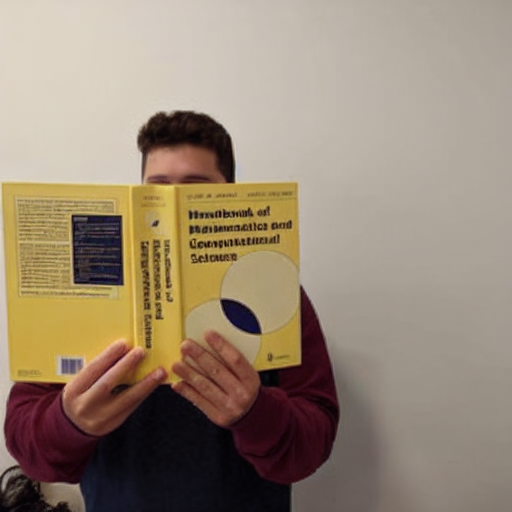
\includegraphics[width=\linewidth]{fig/reconstruction/223000000000.png}
        \\
        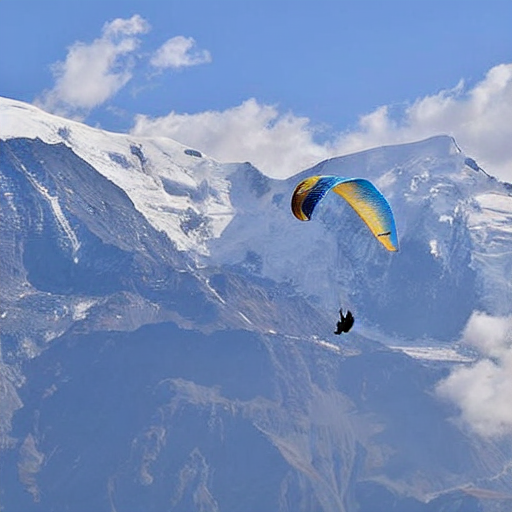
\includegraphics[width=\linewidth]{fig/reconstruction/324000000002_vae.png} & 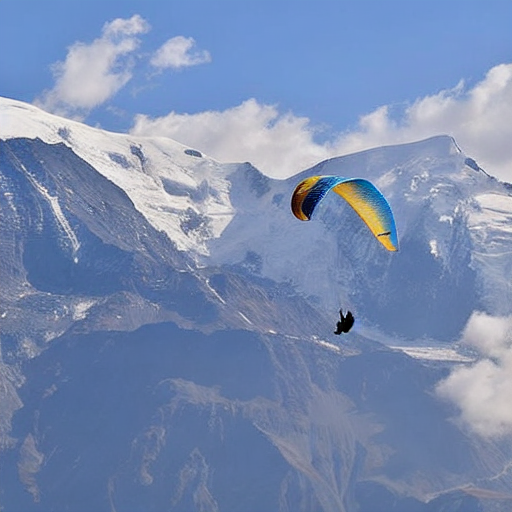
\includegraphics[width=\linewidth]{fig/reconstruction/324000000002.png} &
        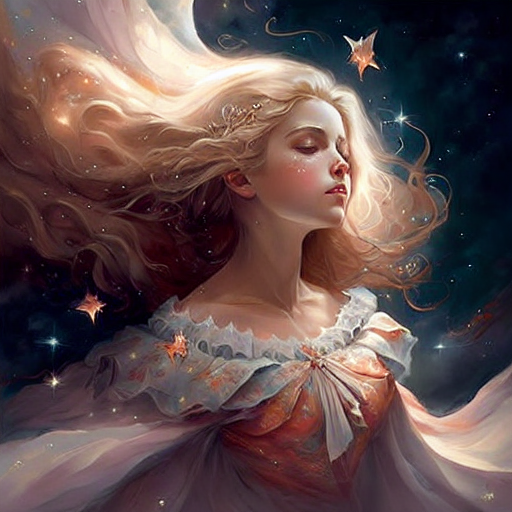
\includegraphics[width=\linewidth]{fig/reconstruction/412000000004_vae.png} & 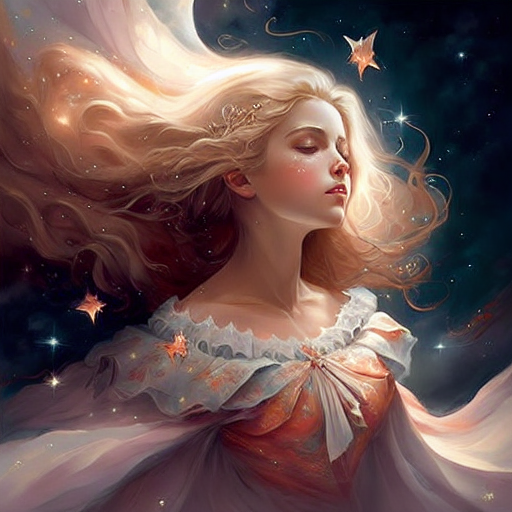
\includegraphics[width=\linewidth]{fig/reconstruction/412000000004.png}
        \\
        \end{tabularx}
    \caption{Reconstruction performance on PieBench samples.}
    % \caption{This figure displays examples where \method{} successfully removes objects from images, a feature not commonly observed in other negative-prompt-based methods. Each example illustrates how the removed element is replaced with content that, unexpectedly, shares structural similarities with the original object. This phenomenon, resulting from the interplay between CFG and SA guidance, highlights a unique aspect of our method's behavior and an opportunity for further refinement.} 
    \label{fig:res_reconstruction}
  \end{figure}

% \begin{table*}[htbp]
%     \centering
%       \renewcommand\arraystretch{0.9}
%       \setlength{\tabcolsep}{0.3mm}{
%     \begin{threeparttable}
%     \begin{tabular}{c|c|cccc|cc}
%     \toprule
%     \toprule
%           & \textbf{Structure}          & \multicolumn{4}{c|}{\textbf{Background Preservation}} & \multicolumn{2}{c}{\textbf{CLIP Similariy}} \\ \midrule
%     \textbf{Method}            & \textbf{Distance}$_{^{\times 10^3}}$ $\downarrow$ & \textbf{PSNR} $\uparrow$     & \textbf{LPIPS}$_{^{\times 10^3}}$ $\downarrow$  & \textbf{MSE}$_{^{\times 10^4}}$ $\downarrow$     & \textbf{SSIM}$_{^{\times 10^2}}$ $\uparrow$    & \textbf{Whole}  $\uparrow$          & \textbf{Edited}  $\uparrow$       \\ \midrule
%     \textbf{Null-text} \cite{mokady2023null} & 13.44           & 27.03  & 60.67  & 35.86  & 84.11 & 24.75        & 21.86          \\
%     \textbf{Negative prompt} \cite{miyake2023negative} &     16.17       &  26.21 &  69.01  &  39.73 & 83.40 &   24.61     &    21.87     \\
%     \textbf{Direct inversion} \cite{ju2023direct} & 11.65           & 27.22  & 54.55  & 32.86  & 84.76 & 25.02         & \textbf{22.10}          \\
%     \textbf{P2P-Zero} \cite{parmar2023zero} & 61.68 & 20.44  & 172.22 & 144.12 & 74.67 & 22.80 & 20.54 \\
%     \textbf{Plug-n-Play} \cite{tumanyan2023plug} \tnote{a} & 28.22 & 22.28  & 113.46 & 83.64 & 79.05 & 25.41 & 22.55 \\
%     \textbf{NegProx} \cite{miyake2023negative} \tnote{b} & \textbf{7.44} & \textbf{28.67} &	41.98 &	\textbf{24.25} &	\textbf{85.98} &	24.28 &	21.36 \\
%     % \textbf{Ours} (temporal) & 24.21 &	25.53 &	62.64 &	55.27 &	83.97 &	\textbf{26.18} &	\textbf{22.86} \\
%     \textbf{Ours} & 10.96 &	27.91 &	\textbf{39.56} &	29.80 &	85.97 &	\textbf{25.47} &	21.96 \\
%     \textbf{Ours} (by task) & 12.70 &	27.67 &	42.30 &	32.09 &	85.71 &	25.75 &	22.37 \\
    
%     \bottomrule
%     \bottomrule
%     \end{tabular}
%     \begin{tablenotes}
%        \footnotesize
%        \item[a] use Stable Diffusion v1.5 as base model (others all use Stable Diffusion v1.4) %revise the source code's 1000 steps to 50 steps
%        \item[b] Proximal guidance with negative prompt as introduced in \cite{han2023proximal}
%         \end{tablenotes}
%     \end{threeparttable}
%     }
%         \vspace{-0.2cm}
%     \caption{Quantitutive analysis performed on PieBench \cite{ju2023direct}. All rows but ours are taken from \cite{ju2023direct}.}
%             \label{tab:comparison_piebench}
%         \vspace{-0.2cm}
%     \end{table*}
    

% \begin{table*}[htbp]
%     \centering
%     \small
%       \renewcommand\arraystretch{0.9}
%       \setlength{\tabcolsep}{0.3mm}{
%     \begin{threeparttable}
%     \begin{tabular}{cccccc}
%    % \toprule
%     \toprule
%           & \textbf{Struct.}          & \multicolumn{2}{c|}{\textbf{Background Preservation}} & \multicolumn{2}{c}{\textbf{CLIP Similariy}} \\ \midrule
%     \textbf{Method}            & \textbf{Distance}$_{^{\times 10^3}}$ $\downarrow$ &   \textbf{LPIPS}$_{^{\times 10^3}}$ $\downarrow$  & \textbf{SSIM}$_{^{\times 10^2}}$ $\uparrow$    & \textbf{Whole}  $\uparrow$          & \textbf{Edited}  $\uparrow$       \\ \midrule
%     \textbf{\nulltextlong} \cite{mokady2023null} & 13.4             & 60.7    & 84.1 & 24.8        & 21.9          \\
%     \textbf{Negative prompt} \cite{miyake2023negative} &     16.2        &  69.0   & 83.4 &   24.6     &    21.9     \\
%     \textbf{\directinversionlong} \cite{ju2023direct} & 11.7             & 54.6    & 84.8 & 25.0         & 22.1          \\
%     \textbf{\ptopzerolong} \cite{parmar2023zero} & 61.7   & 172.2 & 74.7 & 22.8 & 20.5 \\
%     \textbf{\pnplong} \cite{tumanyan2023plug} \tnote{a} & 28.2   & 113.5 & 79.0 & 25.4 & \textbf{22.6} \\
%     \textbf{\negproxlong} \cite{miyake2023negative} \tnote{b} & \textbf{7.4}  &	42.0  &	\textbf{86.0} &	24.3 &	21.4 \\
%     % \textbf{Ours} (temporal) & 24.21 &	25.53 &	62.64 &	55.27 &	83.97 &	\textbf{26.18} &	\textbf{22.86} \\
%     \textbf{\method} (ours) & 11.0 &	\textbf{39.6} &	\textbf{86.0} &	\textbf{25.5} &	22.0 \\
%     % \textbf{Ours} (by task) & 12.70 &	42.30  &	85.71 &	25.75 &	22.37 \\
    
%     \bottomrule
%     %\bottomrule
%     \end{tabular}
%     \begin{tablenotes}
%        \footnotesize
%        \item[a] use Stable Diffusion v1.5 as base model (others all use Stable Diffusion v1.4) %revise the source code's 1000 steps to 50 steps
%        \item[b] Proximal guidance with negative prompt as introduced in \cite{han2023proximal}
%         \end{tablenotes}
%     \end{threeparttable}
%     }
%         \vspace{-0.2cm}
%     \caption{Quantitative analysis performed on PieBench \cite{ju2023direct}. All rows but ours are taken from \cite{ju2023direct}.}
%             \label{tab:comparison_piebench}
%         \vspace{-0.2cm}
%     \end{table*}




    \begin{table}[htbp]
        
    \centering
    \small
      \renewcommand\arraystretch{0.9}
      \setlength{\tabcolsep}{0.5mm}{
  \resizebox{\linewidth}{!}{  \begin{tabular}{cccccc}
   % \toprule
    \toprule
        %   & \multicolumn{4}{c}{\textbf{Structure}} & \textbf{CLIP Similariy} \\ \midrule
    \textbf{Method}            & \textbf{Struc. dist.} $\downarrow$ &   \textbf{PSNR} $\uparrow$  & \textbf{LPIPS} $\downarrow$    & \textbf{MSE}  $\downarrow$          & \textbf{SSIM}  $\uparrow$       \\ \midrule
    \textbf{VAE reconstruction} & \textbf{2.8} & \textbf{27.2} & \textbf{40.2} & \textbf{28.5} & \textbf{79.8} \\
    \textbf{\directinversionlong} \cite{ju2023direct} & 3.0 & 27.1 & 51.7 & 28.9 & 79.5\\
    \textbf{\nulltextlong} \cite{parmar2023zero} & 3.3 & 26.7 & 54.8 & 31.1 & 78.9 \\
    \textbf{\method} (ours) & 12.0 & 24.7 & 65.8 & 65.1 & 77.47\\
    
    \bottomrule
    %\bottomrule
    \end{tabular}}

    }
        % \vspace{-0.2cm}
    \caption{
        Performance of different models on PieBench samples, specifically evaluating reconstruction quality only ($\pin$ and $\pout$ are the same).
    }
            
            \label{tab:res_reconstruction}
        % \vspace{-0.2cm}
    \end{table}


  


\subsection{Self-attention guidance for reconstruction}
\label{sec:sup_reconstruction}
% In Fig \ref{fig:res_reconstruction} we compare SAGE's reconstruction performance when using the same input and editing prompt to the bare VAE reconstruction. In this evaluation, no local blending or other auxiliary techniques are applied, only self-attention guidance. The results demonstrate that SAGE can faithfully reconstruct fine details, despite not explicitly optimizing for reconstruction as \nulltextlong{} or accounting for the VAE reconstruction error as \directinversionlong{} methods do. Quantitatively, our method performs worse than these baselines in strict reconstruction metrics (see Table \ref{tab:res_reconstruction}), as they directly target the VAE latent space. However, this difference has no noticeable impact on the final editing quality, as it could be assessed in Tables \ref{tab:comparison_piebench}, \ref{tab:comparison_magicbrush} and \ref{tab:user_study} where \method{} outperform the compared methods, particularly on the reconstruction metrics.
Figure~\ref{fig:res_reconstruction} compares the reconstruction performance of \method{} given the same input image and editing prompt against the baseline VAE reconstruction. This evaluation applies only self-attention guidance, without local blending or auxiliary techniques. The results clearly show that SAGE preserves fine details despite not explicitly optimizing for reconstruction like \nulltextlong{} or compensating for VAE reconstruction errors as \directinversionlong{} does. Although our method performs worse on strict reconstruction metrics (Table~\ref{tab:res_reconstruction}) due to its indirect approach, this has no noticeable impact on final editing quality. As shown in Tables~\ref{tab:comparison_piebench}, \ref{tab:comparison_magicbrush}, and \ref{tab:user_study}, the proposed method outperforms the compared methods, particularly in reconstruction-related evaluations.





% \subsection{PieBench Examples}
% \label{sec:sup_results_piebench}

% \input{fig/ex_all1.tex}
% % \input{fig/ex_all2.tex}

% In Figure \ref{fig:sup_exall1} we show additional qualitative examples of the results corresponding to the images generated with the complete SAGE method variant \textit{(vi)} (see Table \ref{tab:ablation_piebench} of the main paper) and used for computing the metrics in Tables \ref{tab:ablation_piebench}, \ref{tab:comparison_piebench}, and \ref{tab:user_study} of the main manuscript. Our understanding is that as the self-attention maps mostly encode low-resolution semantic features instead of shapes, SAGE is able to generate images that better capture the style while changing the content (as the fox in the second row of Fig~\ref{fig:sup_exall1}), has more freedom to edit the shape of elements (as the tulips in the third row of Fig~\ref{fig:sup_exall1}), and is able to eliminate elements that are present in the original image while filling the gap with plausible content (as the camera in the last row of Figs~\ref{fig:sup_exall1} and~\ref{fig:sup_structpres}). Similarly, SAGE is the only method capable of applying pixel-art style (clown in Fig~\ref{fig:sup_exall1}). Further confirmation of our hypothesis that self-attention maps encode low-resolution semantic features is provided by the fact that SAGE changes not only the style of the last row of Fig~\ref{fig:sup_exall1} but also substantially changes the kind of chair (from modern to classic) to better fit the style of the new prompt.

% \subsection{Direct Inversion comparison}
% \label{sec:sup_results_di}

% Discuss the results of the direct inversion comparison and include the discussion with the time/mem fp16 analysis. \ref{fig:sup_ex_di_comp}.
% \directinversion{} exhibits competitive performance compared to \method{}, both in quantitative metrics and user evaluations. However, \directinversion{} struggles in specific scenarios due to its approach to content preservation through $\vz$-space reconstruction. \directinversion's performance is bound to reconstruction of the input image in the high-resolution latent $\vz$-space, which, while effective in many contexts, falls short when deviations from the source shape are required. Unlike \directinversion{}, \method{} operates on self-attention maps within a semantically-rich, lower-resolution space, affording it superior adaptability in situations where pixel-perfect accuracy is detrimental. For instance, \directinversion's limitations become evident when attempting pixel-art style transformations (as shown in Figure \ref{fig:sup_exall1}), where its inherent constraints on divergence hinder the editing of the target image style. Similarly, Figure \ref{fig:sup_ex_di_comp} highlights DI's inadequacies in image edits involving significant shape alterations or object removal, where its reliance on close adherence to the input image's structural integrity limits effective modifications.

% Even though the simpler \textit{three-code-lines} approach of DI \cite{ju2023direct} grants it a slight edge in computational efficiency, \method{}'s superior adaptability and flexibility in image editing scenarios, as well as its competitive performance in time and memory consumption, position it as a more versatile and effective solution for prompt-guided image editing.

% \input{fig/ex_di_comp.tex}

% \newpage
% \input{fig/selfreplace_fig.tex}
% \subsection{Ablation Analysis}
% \label{sec:sup_results_ablation}

% \paragraph{Self-attention replace} In Figures \ref{fig:supablation_selfreplace} we show the results of replacing the self-attention (as in \cite{hertz2023prompt}) instead of guiding the reconstruction towards them as described in Sec~\ref{sec:self_attention_guidance}. CFG $w$ values between $0$ (only $\pin$) and $1$ (only $\pout$) are able to generate plausible interpolation between both but with really poor prompt fidelity (as expected), whereas for $w$ values higher than 1, the generation quality is really poor, with oversaturated colors and artifacts. This is most likely due to the fact that direction of the second added of Eq~\ref{eq:cfg} is too high as both $\pin$ and $\pout$ self-attention maps are misaligned (guidance results in a softer difference). To solve this, \cite{hertz2023prompt} replaces the self-attention maps of both $\pin$ (or $\varnothing$) and $\pout$ inducing the need of a whole reconstruction stage (see Fig~\ref{fig:related}), not only the $\pin$ branch as we do (see Fig~\ref{fig:method_diag}).


% \paragraph{CFG and Attention reweighting} 
% %In Figure \ref{fig:supablation_cfg_weight}, we show the impact of CFG (Sec \ref{sec:self_attention_guidance}) and Attention Reweighting (Sec \ref{sec:cross_attention_manipulation}) in the generation process. Both techniques are able to increase the attention to $\pout$ but their procedure and impact is different. We show how CFG achieves more natural looking result, whereas in our example attention reweighting results in dog-features leaking to the goat. In our experience, attention reweighting should be reserved to situations where further increasing the CFG would result in unnatural results and oversaturated colors or artifacts as it usually yields better editing. If CFG is not enough, then it is better to decrease the CFG and apply attention reweighting to increase the attention to some $\pout$ key words, otherwise unnatural-looking colors are amplified when both parameters are high.
% \input{fig/competing_terms_fig.tex}
% \input{fig/cfg_weight_matrix.tex}

% In Figure \ref{fig:supablation_competing}, we illustrate the competing and coordinated nature of self-attention guidance and the Classifier-Free guidance. In Figure \ref{fig:supablation_competing_self}, we can see how self-attention guidance works through the entire image to reconstruct the input image, whereas in Figure \ref{fig:supablation_competing_cfg}, we can see how Classifier-Free guidance works only in the areas corresponding to semantic editing.

\section{Limitations}
\subsection{Structure Preservation}
\label{sec:sup_limitations_structure}


    Figure~\ref{fig:sup_structpres} shows that when objects are removed by omitting corresponding words from the prompt, \method{} fills the resulting gaps with content that maintains structural similarities to the removed elements. This behavior likely arises from a conflict between CFG—which pushes for object removal—and self-attention guidance—which favors preserving the original structure. Despite this unintended effect, \method{} is the only approach among those compared that actually removes objects, whereas other negative-prompt-based methods fail to do so. Future work may address this by selectively masking self-attention guidance in areas corresponding to the removed elements, similar to the local blending strategy.

\setlength{\tabcolsep}{1pt}
\begin{figure}[h]
    \footnotesize
    \small
    % \begin{tabular}{*{6}{p{2.8cm}}}
    %   \hline
    %   & & & & & \\
    %   \centering Input & \centering \ptopzero & \centering \nulltext & \centering  \directinversion & \centering  \negprox & \centering \method{} \\
    %   %   \multicolumn{6}{c}{``\textit{A \textcolor{RoyalBlue}{\textbf{lego}} cat \textcolor{RoyalBlue}{\textbf{toy}} sitting next to a mirror}"} \\
    %   \multicolumn{6}{c}{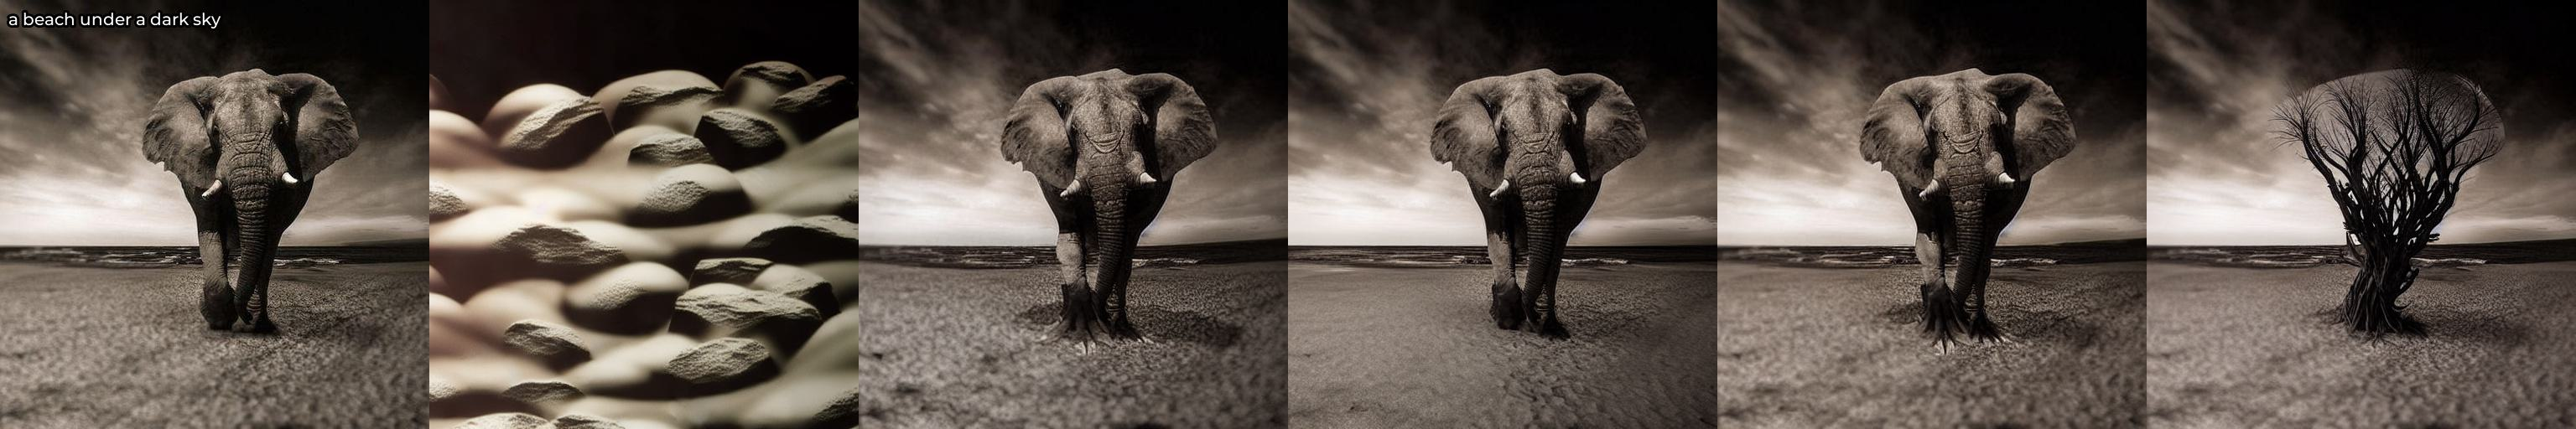
\includegraphics[width=\linewidth]{fig/ex_structpres/3_delete_object_80-2_natural-1_animal-321000000005}} \\
    % \multicolumn{6}{c}{}  \\
    % % 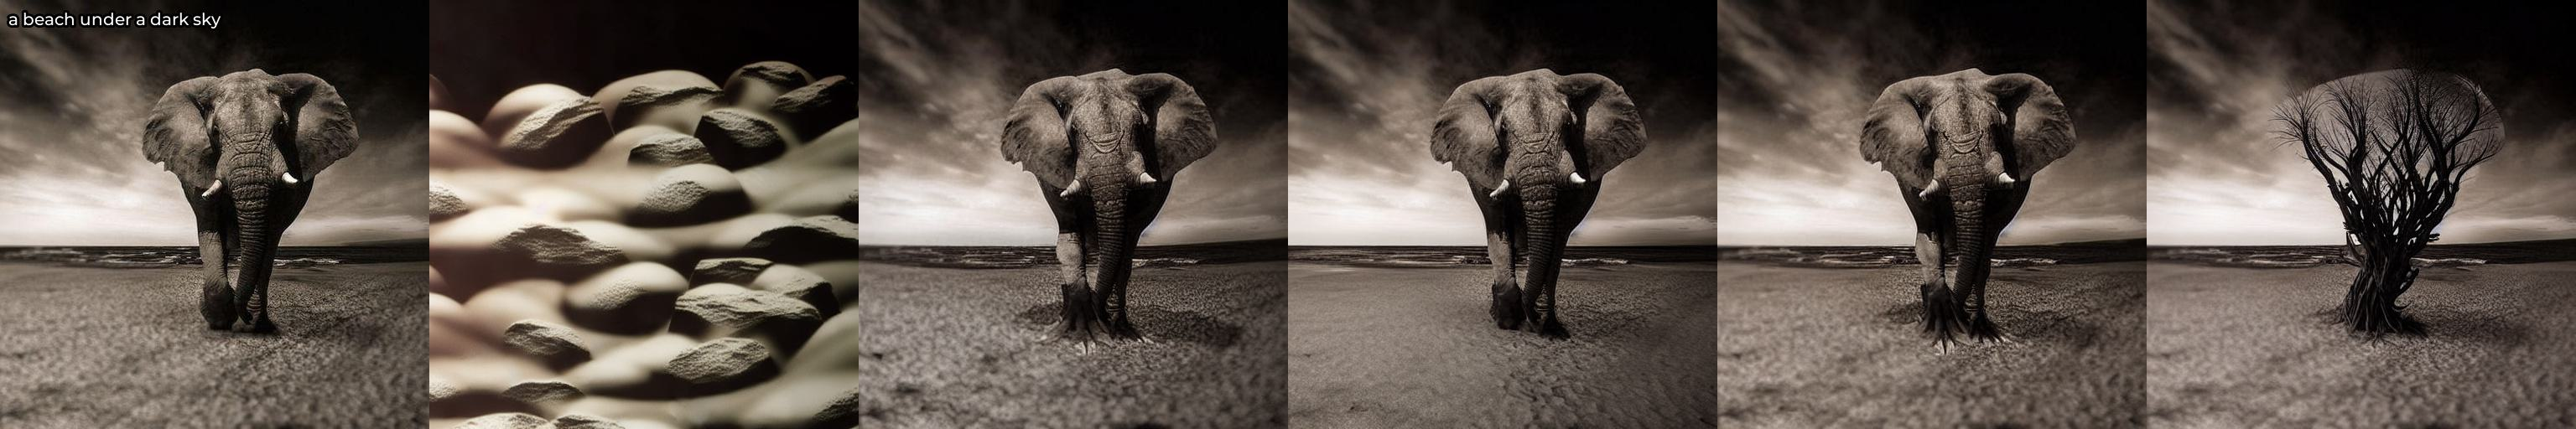
\includegraphics[height=2.2cm]{fig/ex_structpres/3_delete_object_80-2_natural-1_animal-321000000005} \\
    % %   \multicolumn{6}{c}{``\textit{Orange van with \textcolor{BrickRed}{\st{surfboards}} \textcolor{RoyalBlue}{\textbf{flowers}} on top}"} \\
    % %   \insertimage{van}{input}\\
    % %   \multicolumn{6}{c}{``\textit{Meat \textcolor{BrickRed}{\st{balls}} \textcolor{RoyalBlue}{\textbf{shushi}} on white plate}"} \\
    % %   \insertimage{meat}{input}\\
    % %   \multicolumn{6}{c}{``\textit{A \textcolor{BrickRed}{\st{woman}} \textcolor{RoyalBlue}{\textbf{storm-trooper}} with blue hair}"} \\
    % %   \insertimage{girl}{input}\\
    % %   \multicolumn{6}{c}{``\textit{A \textcolor{BrickRed}{\st{cat}} \textcolor{RoyalBlue}{\textbf{dog}} sitting on a wooden chair}"} \\
    % %   \insertimage{cat2}{input}\\
    %   \hline
    %   % ... Add more rows as needed
    % \end{tabular}
    \begin{tabularx}{\columnwidth}{ YYYYYY }
        Input & \ptopzero &  \nulltext &  \directinversion &  \negprox &  \method \\
        \multicolumn{6}{c}{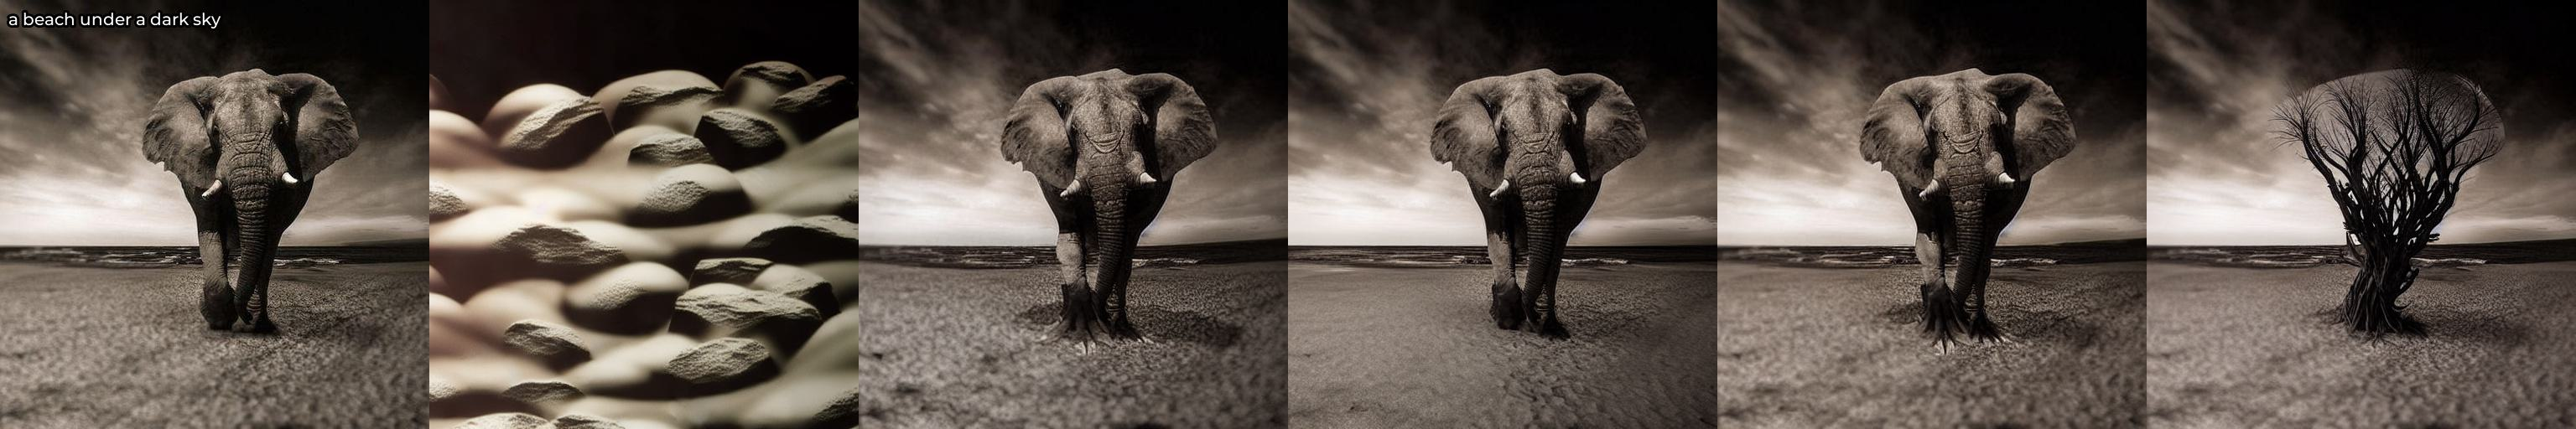
\includegraphics[width=\linewidth]{fig/ex_structpres/3_delete_object_80-2_natural-1_animal-321000000005}} \\
        \multicolumn{6}{c}{``\textit{\textcolor{BrickRed}{\st{an elephant walking on}} a beach under a dark sky}"} \\
        \multicolumn{6}{c}{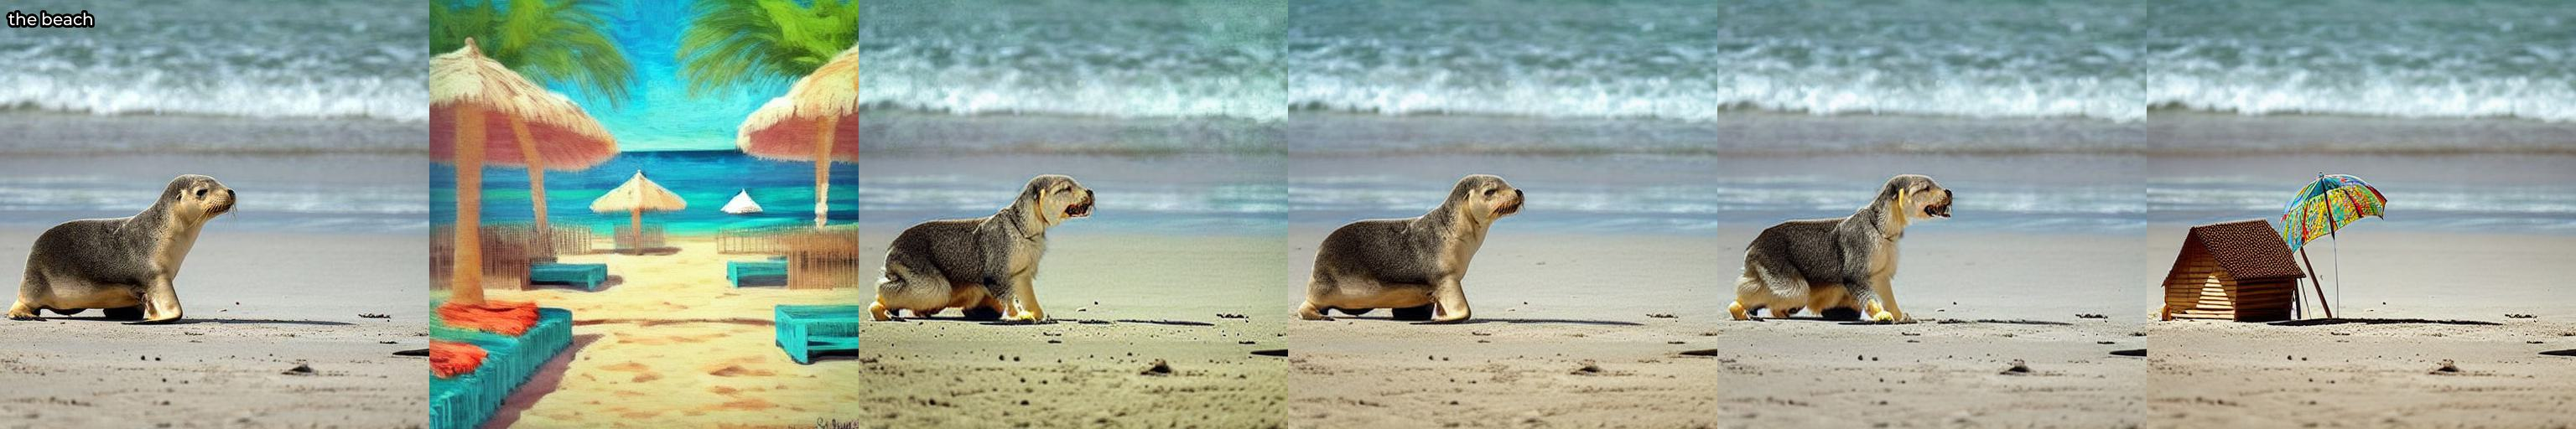
\includegraphics[width=\linewidth]{fig/ex_structpres/3_delete_object_80-2_natural-1_animal-321000000006}} \\
        \multicolumn{6}{c}{``\textit{\textcolor{BrickRed}{\st{a seal pup on}} the beach}"} \\
        
        \end{tabularx}
    % \caption{PieBench examples. STRUCTURE PRESERVATION.}
    \caption{Examples of object removal by \method{}. Although the method inadvertently fills gaps with structurally similar content, likely due to the complex interplay between CFG and self-attention guidance, it remains the only approach that consistently and effectively removes target objects.}
    \label{fig:sup_structpres}
  \end{figure}

\subsection{Failure Cases}
\label{sec:sup_limitations_failure}

\setlength{\tabcolsep}{1pt}
\begin{figure}[h]
    \footnotesize
    \begin{tabularx}{\columnwidth}{ *{6}{Y} }
        Input & \ptopzero &  \nulltext &  \directinversion &  \negprox &  \method \\
        \multicolumn{6}{c}{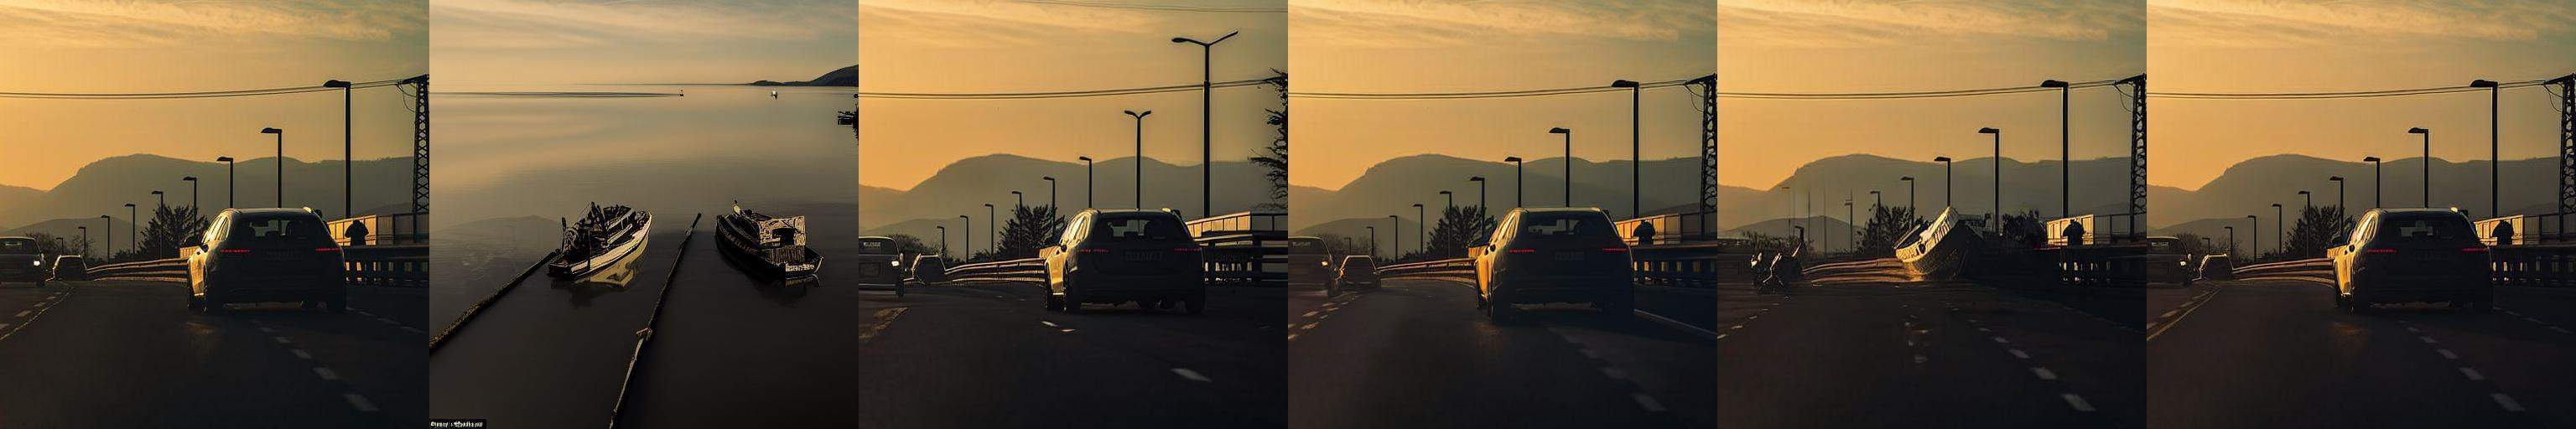
\includegraphics[width=\linewidth]{fig/ex_fail/all/1_change_object_80-2_natural-4_outdoor-124000000000}} \\
        \multicolumn{6}{c}{``\textit{\textcolor{BrickRed}{\st{cars}} \textcolor{RoyalBlue}{\textbf{boats}} driving on a highway at sunset}"} \\
        \multicolumn{6}{c}{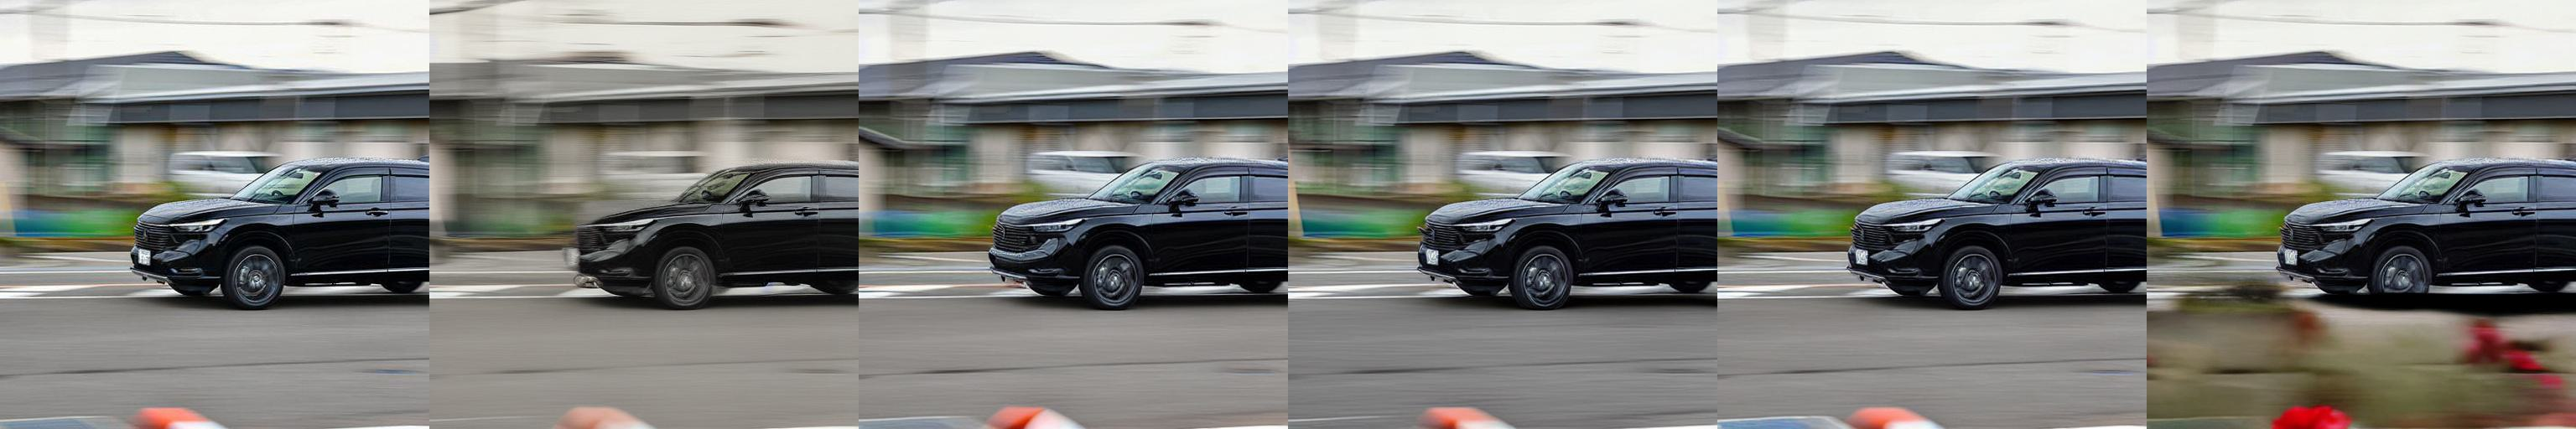
\includegraphics[width=\linewidth]{fig/ex_fail/all/7_change_attribute_material_40-2_natural-4_outdoor-724000000002}} \\
        \multicolumn{6}{c}{``\textit{the 2020 honda hrx is driving down the road \textcolor{RoyalBlue}{\textbf{full of flowers}}}"} \\
        \multicolumn{6}{c}{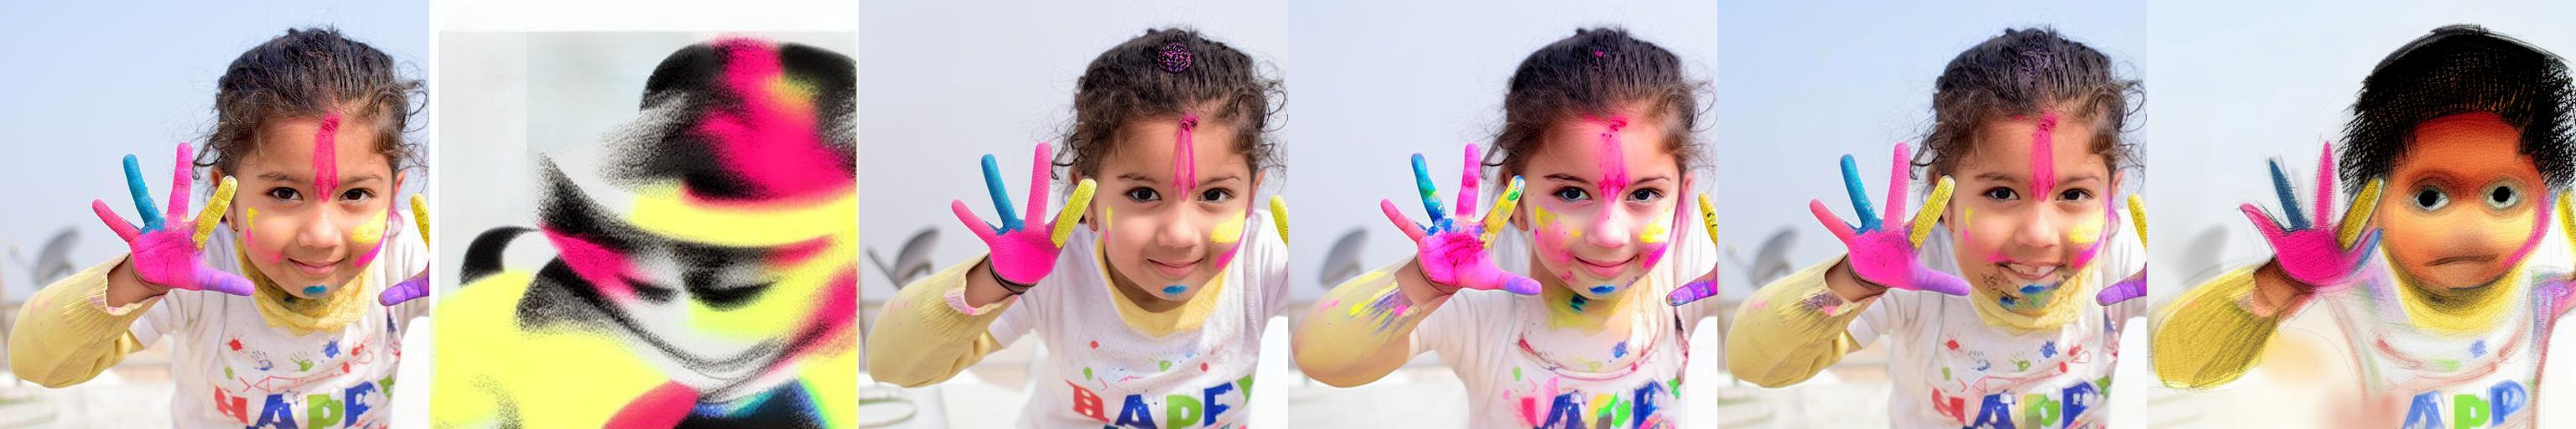
\includegraphics[width=\linewidth]{fig/ex_fail/all/9_change_style_80-2_natural-2_human-922000000009}} \\
        \multicolumn{6}{c}{``\textit{\textcolor{RoyalBlue}{\textbf{black and white sketch of}} a young girl with painted hands and face}"} \\
        \multicolumn{6}{c}{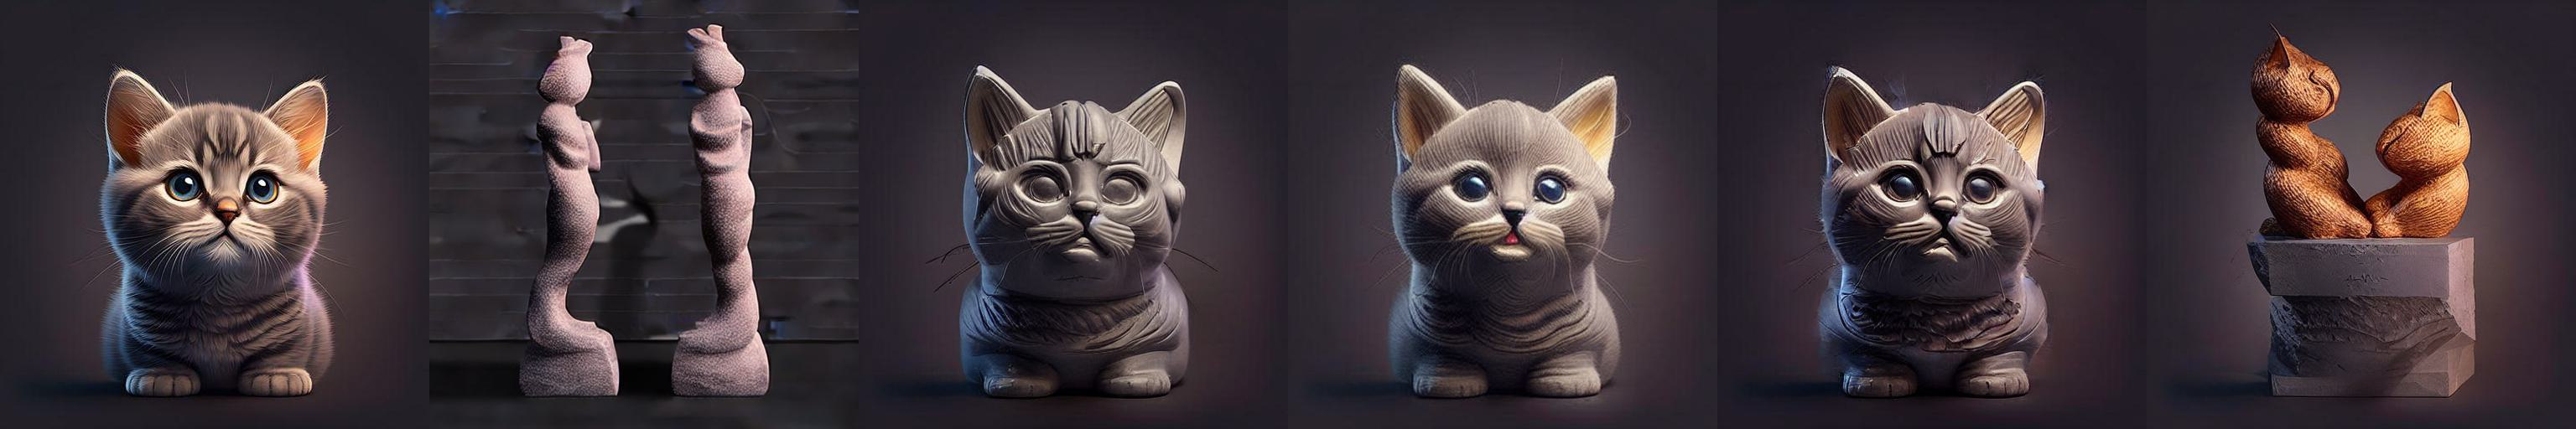
\includegraphics[width=\linewidth]{fig/ex_fail/us/7_change_attribute_material_40-1_artificial-1_animal-711000000004}} \\
        \multicolumn{6}{c}{``\textit{a kitten \textcolor{RoyalBlue}{\textbf{sculpture}} }"} \\
        \multicolumn{6}{c}{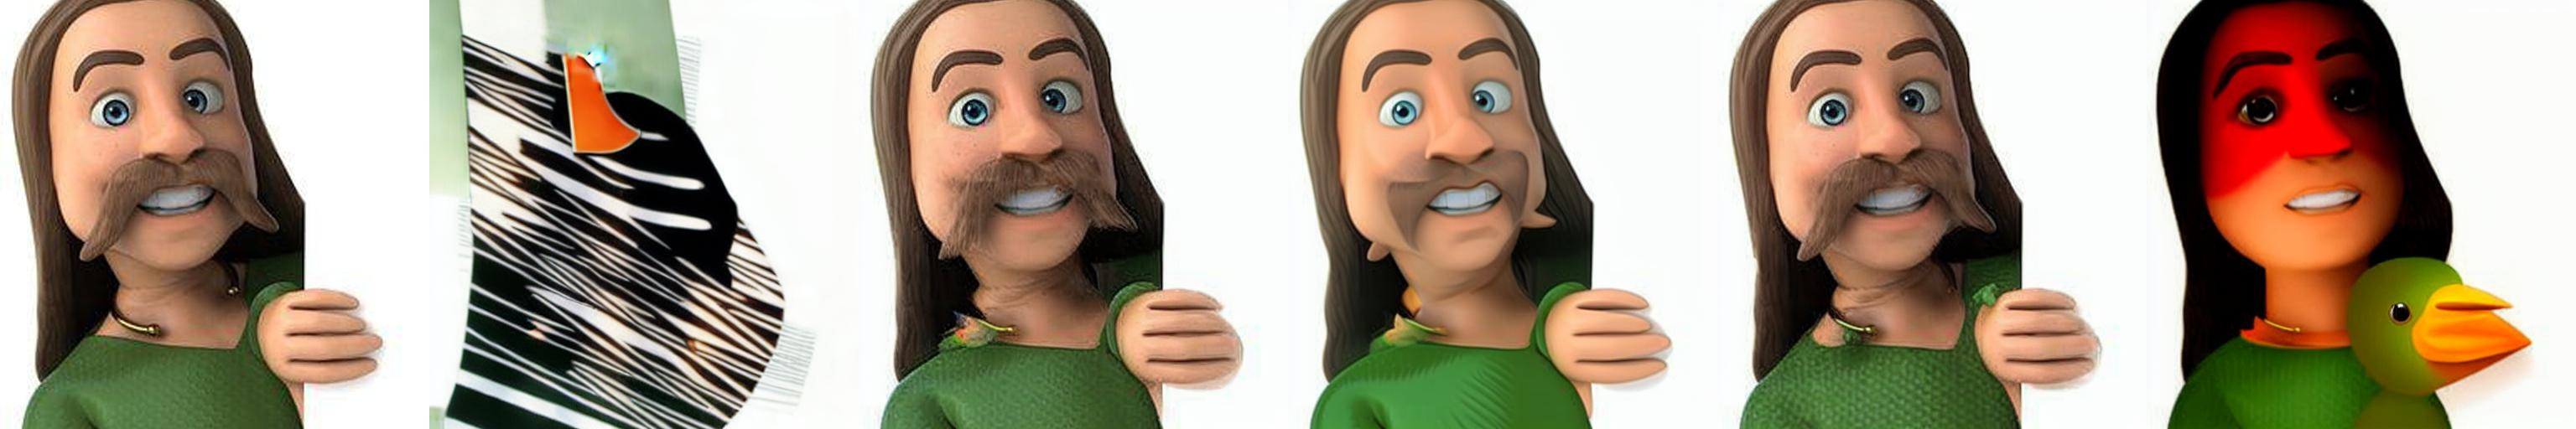
\includegraphics[width=\linewidth]{fig/ex_fail/satur/2_add_object_80-1_artificial-2_human-212000000008}} \\
        \multicolumn{6}{c}{``\textit{a cartoon man \textcolor{RoyalBlue}{\textbf{and a bird}}}"} \\
        \end{tabularx}
        \caption{This figure presents examples from the PieBench dataset where various methods, including ours, encounter difficulties in achieving the desired editing outcomes. These images highlight the challenges and limitations faced in specific editing scenarios, providing insights into areas where each method may require further refinement or adaptation.}
        % \caption{Examples from the PieBench dataset highlighting failure cases across different methods. The figure shows scenarios where the intended edits are not achieved due to the sensitivity of CFG-based approaches to hyperparameter choices. In rare instances, SAGE produces oversaturated and poorly reconstructed images—issues that can be alleviated by reducing the CFG weight ($w$) and self-attention guidance ($\lambda$).}
    \label{fig:sup_exfailall}
  \end{figure} 

% As discussed in Sections \ref{sec:limitations} of the main paper of supplementary materials, CFG-based methods are sensitive to the hyperparameters used for generation. This is specially true in the compared methods as they all include additional parameters for the editing or reconstruction. In Figure \ref{fig:sup_exfailall} we show some examples of the images corresponding to the PieBench dataset where the different methods strugle to achieve the required editing. In most of the cases, at least for SAGE, the problem can be solved by a different choice of parameters, but this is not plausible in large-scale quantitative evaluations.

% \input{fig/ex_fail_us.tex}
% In a smaller extent, we find examples where SAGE performs significantly worse than some other method. This is specially true for editings where changes are small or have fine details as \textit{spiderman} or the \textit{moon} in Figure \ref{fig:sup_exfailus}.

% \input{fig/ex_fail_satur.tex}
%Finally, we have observed that in a few cases, when all the methods fail (as happened in Fig~\ref{fig:sup_exfailall}), SAGE displays a failing behaviour different to the rest of methods. In Figure \ref{fig:sup_exfailsatur} we show some examples of this behaviour. The resulting images are oversaturated and poorly reconstructed. In these cases, the problem can be solved by reducing significantly both the CFG $w$ and Self-attention guidance $\lambda$ values.
% Finally, we have observed distinct failure patterns in SAGE, particularly in scenarios where all methods struggle. In a few cases (only 6 out of the 700 PieBench examples), SAGE tends to produce oversaturated and poorly reconstructed images, as exemplified in the last row of Fig. \ref{fig:sup_exfailall}. These issues are notably different from the failure modes of other methods. Fortunately, we found that significantly reducing both CFG $w$ and self-attention guidance $\lambda$ values can effectively address these problems, offering a viable solution for these specific failure cases.

CFG-based editing methods are inherently sensitive to hyperparameter settings, especially when additional parameters control editing or reconstruction. Figure~\ref{fig:sup_exfailall} presents examples from the PieBench dataset where various methods, including ours, struggle to achieve the intended edits. In many cases, tuning parameters can resolve the issues for SAGE, but such fine-tuning is impractical for large-scale evaluations. Notably, in a small fraction of cases (6 out of 700), SAGE produces oversaturated and poorly reconstructed images—a distinct failure mode compared to other methods. We found that significantly reducing both the CFG weight ($w$) and the self-attention guidance ($\lambda$) effectively mitigates these problems, indicating a promising direction for further refinement.

% \input{sec/X_rebuttal_2.tex}


\end{document}
